\documentclass[a4paper, 12pt,twoside]{article}
\usepackage[T2A,T1]{fontenc}
\usepackage[utf8]{inputenc}
\usepackage[english, russian]{babel}
\usepackage{graphicx}
\usepackage[hcentering, bindingoffset = 10mm, right = 15 mm, left = 15 mm, top=20mm, bottom = 20 mm]{geometry}
\usepackage{multirow}
\usepackage{lipsum}
\usepackage{amsmath, amstext}
\usepackage{siunitx}
\usepackage{subcaption}
\usepackage{wrapfig}
\usepackage{adjustbox}
\usepackage{enumerate, indentfirst, float}
\usepackage{capt-of, svg}
\usepackage{pscyr} % Нормальные шрифты

\usepackage[normalem]{ulem} % для подчёркиваний uline
\ULdepth = 0.16em

\usepackage{fancyhdr} %Колонтикулы
\pagestyle{fancy}
\lhead{
\includegraphics[width = 10 mm]{logo.jpg} Лабораторная работа № 3.6.1}
\rhead{\textit{\today}}

\newenvironment{bottompar}{\par\vspace*{\fill}}{\clearpage}
 
\begin{document}
\begin{titlepage}

\newcommand{\HRule}{\rule{\linewidth}{0.7mm}} % Defines a new command for the horizontal lines, change thickness here

\center % Center everything on the page
 
%----------------------------------------------------------------------------------------
%	HEADING SECTIONS
%----------------------------------------------------------------------------------------

\textsc{\LARGE Московский Физико-Технический Институт}\\[1,5cm] % Name of your university/college
\textsc{\Large Кафедра общей физики}\\[0.5cm] % Major heading such as course name
\textsc{\large Лабораторная работа \textnumero  3.6.1}\\[0.5cm] % Minor heading such as course title

%----------------------------------------------------------------------------------------
%	TITLE SECTION
%----------------------------------------------------------------------------------------

\HRule
\\[0.4cm]
{ \huge \bfseries Спектральный анализ электрических сигналов}
\\[0.2cm] % Title of your document
\HRule
\\[1.5cm]


 
%----------------------------------------------------------------------------------------
%	AUTHOR SECTION
%----------------------------------------------------------------------------------------

\begin{minipage}{0.4\textwidth}
	\begin{flushleft} \large
		\textbf{Автор:}\\
		Глеб Уваркин \\
		615 группа
	\end{flushleft}
\end{minipage}
~
\begin{minipage}{0.4\textwidth}
	\begin{flushright} \large
		\textbf {Преподаватель:} \\
		Андрей Александрович Заболотных % Supervisor's Name
	\end{flushright}
\end{minipage}

\begin{bottompar}
	\begin{center}
		
\includegraphics[width = 80 mm]{logo.jpg}
	\end{center}
	{\large \today}

\end{bottompar}
\vfill % Fill the rest of the page with whitespace

\end{titlepage}


{\Large \uline { \textbf  {Цель работы:}}}

\vspace{2mm}

Изучить спектральный состав периодических электрических сигналов различной формы: последовательности прямоугольных импульсов, последовательности цугов и амплитудно - модулированных гармонических колебаний.

\vspace{\baselineskip}

{\Large \uline { \textbf  {В работе используются:}}}

\vspace{2mm}

Анализатор спектра, генератор прямоугольных импульсов, генератор сигналов специальной формы, осциллограф.

\section{Теоретические сведения.}

\subsection{Спектральный анализ.}

Рассмотрим функцию вида:
$$f(t) = A_{1}cos(\omega_1t-\alpha_{1}) + ... + A_{n}cos(\omega_{n}t-\alpha_{n})$$
или в более короткой записи:
$$f(t) = \sum\limits_{i=1}^n A_{i}cos(\omega_{i}t-\alpha_{i})$$
где $A_{i}, \omega_{i}, \alpha_{i}$ - постоянные величины. Множество пар $(\omega_{i}, A_{i}), \: i \in 1..N$ - называется спектром функции $f(t)$.

\subsection{Периодические сигналы.}

В физике широко используется разложение сложных сигналов на гармонические колебания различных частот $\omega$. Представление периодического сигнала в виде суммы гармонических сигналов в математике называется разложением в \textit {ряд Фурье}

Пусть заданная функция $f(t)$ - периодически повторяется с частотой $\Omega_{1}=\frac{2\pi}{T}$, где $T$ - период повторения сигнала $f(t)$
Её разложение в ряд Фурье имеет вид:
\begin{equation}
\label{form:furie}	
	f(t)=\frac{a_{0}}{2}+\sum\limits_{n=1}^{\infty}[a_{n}\cos(n\Omega_{1}t)+b_{n}\sin(n\Omega_{1}t)] 
\end{equation}

или
\begin{equation}
	f(t)=\frac{a_{0}}{2}+\sum\limits_{n=1}^{\infty}A_{n}\cos(n\Omega_{1}t-\psi_{n}) 
\label{form:furie_2}
\end{equation}

Здесь $\frac{a_{0}}{2}$ - среднее значение функции $f(t)$. Постоянные $a_n$ и $b_n$ определяются выражениями:
\begin{equation}
\label{form:a_n}
	a_{n} = \frac{2}{T}\int\limits_{t_{1}}^{t_{1}+T}f(t)\cos(n\Omega_1t)\, dt
\end{equation}

\begin{equation}
	b_{n} = \frac{2}{T}\int\limits_{t_{1}}^{t_{1}+T}f(t)\sin(n\Omega_{1}t)\, dt 
\label{form:b_n}
\end{equation}

Точку начала интегрирования $t_{1}$ можно выбрать произвольно.

\begin{equation}
\label{form:A_n}
	A_{n} = \sqrt{a_{n}^2+b_{n}^2}
\end{equation}
\begin{equation}
	\psi_{n} = \arctan\frac{b_{n}}{a_{n}}
\label{form:psi_n}
\end{equation}

\section{Ход работы.}
\subsection{Исследование спектра периодической последовательности прямоугольных импульсов.}

$V_0$  - амплитуда, $\tau$ - длительность, $\Omega_{1} = \frac{2\pi}{T} $ - частота повторения, где $T$-период повторения импульсов.

Согласно формуле (\ref{form:a_n}) находим:
$$ \langle V \rangle = \frac{a_0}{2} = \frac{A_0}{2} = \frac{1}{T}\int\limits_{ -\frac{\tau}{2}}  ^ {\frac{\tau}{2} } V_0\,dt = V_0 \frac{\tau}{T}
$$

Коэффициенты при косинусных составляющих равны
\begin{equation}
\label{form:app_a_n}
	a_n = \frac{2}{T}\int\limits_{ -\frac{\tau}{2} } ^ {\frac{\tau}{2} } V_0\cos(nf_\text{повт}t)\, dt \sim \frac{\sin(x)}{x}
\end{equation}
 
В силу чётности функции $\forall n \in {N} \ b_n=0$. Таким образом, спектр периодической последовательности прямоугольных импульсов должен выглядеть как график $\frac{\sin(x)}{x}$.
\subsubsection*{Выполнение.}
В работе используются: \textit{анализатор спектра СК4-56; генератор прямоугольных импульсов Г5-54; осциллограф}



\begin{figure}[H]
\centering
\includegraphics[width = 0.8\textwidth]{schemeA}
\caption{Схема для исследования спектра периодической последовательности прямоугольных импульсов}
\label{img:scheme A}
\end{figure}

Собираем схему согласно рис. \ref{img:scheme A}. Получаем на экране осциллографа последовательность периодических прямоугольных импульсов. Подключаем анализатор спектра СК4-56 и после настройки наблюдаем спектр сигнала с параметрами: $$f_\text{повт} = 10^3 \; \text{Гц}, \tau = 25 \; \text{мкс}, m_x = 5 \; \frac{\text{кГц}}{\text{дел}}$$

\newpage

\begin{figure}[h]
	\centering
	\begin{minipage}[h]{0.30\linewidth}
		\centering{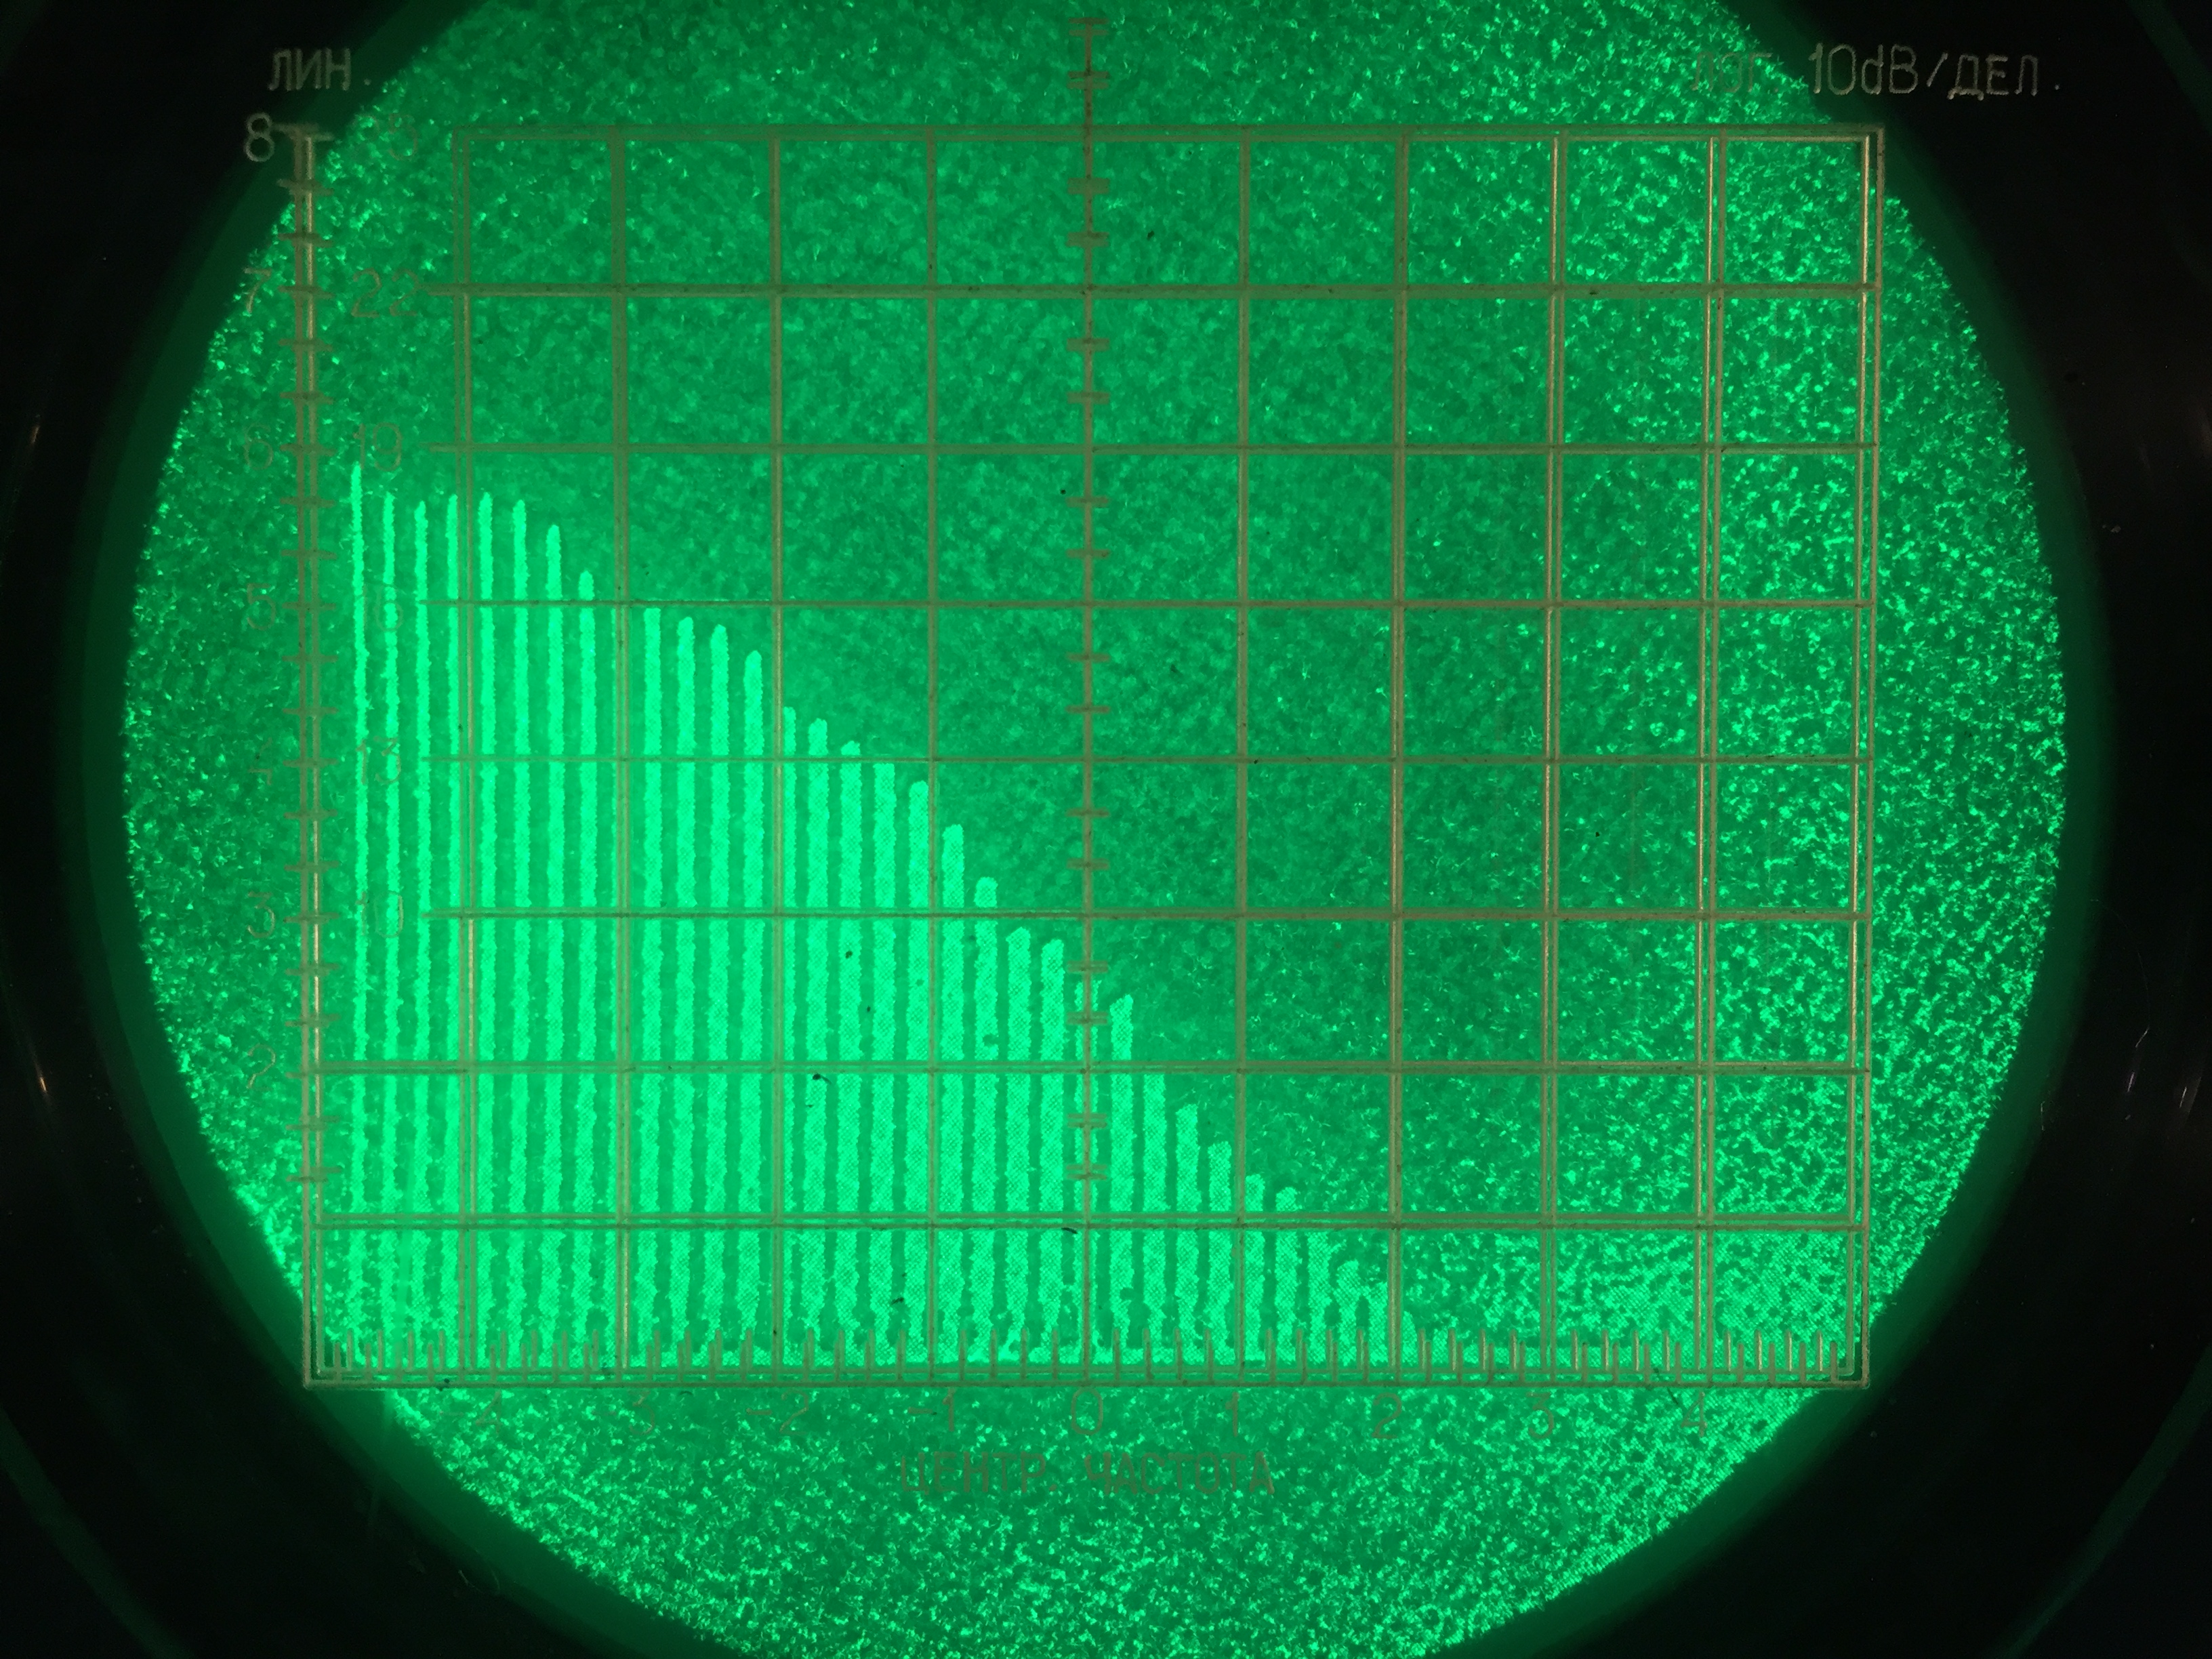
\includegraphics[width=0.9\linewidth]{IMG_0622} \\ $f_{\text{повт}}=1\text{кГц}$ \\ $ \tau = 25 \text{мкс}$}
	\end{minipage}
	\begin{minipage}[h]{0.30\linewidth}
		\centering{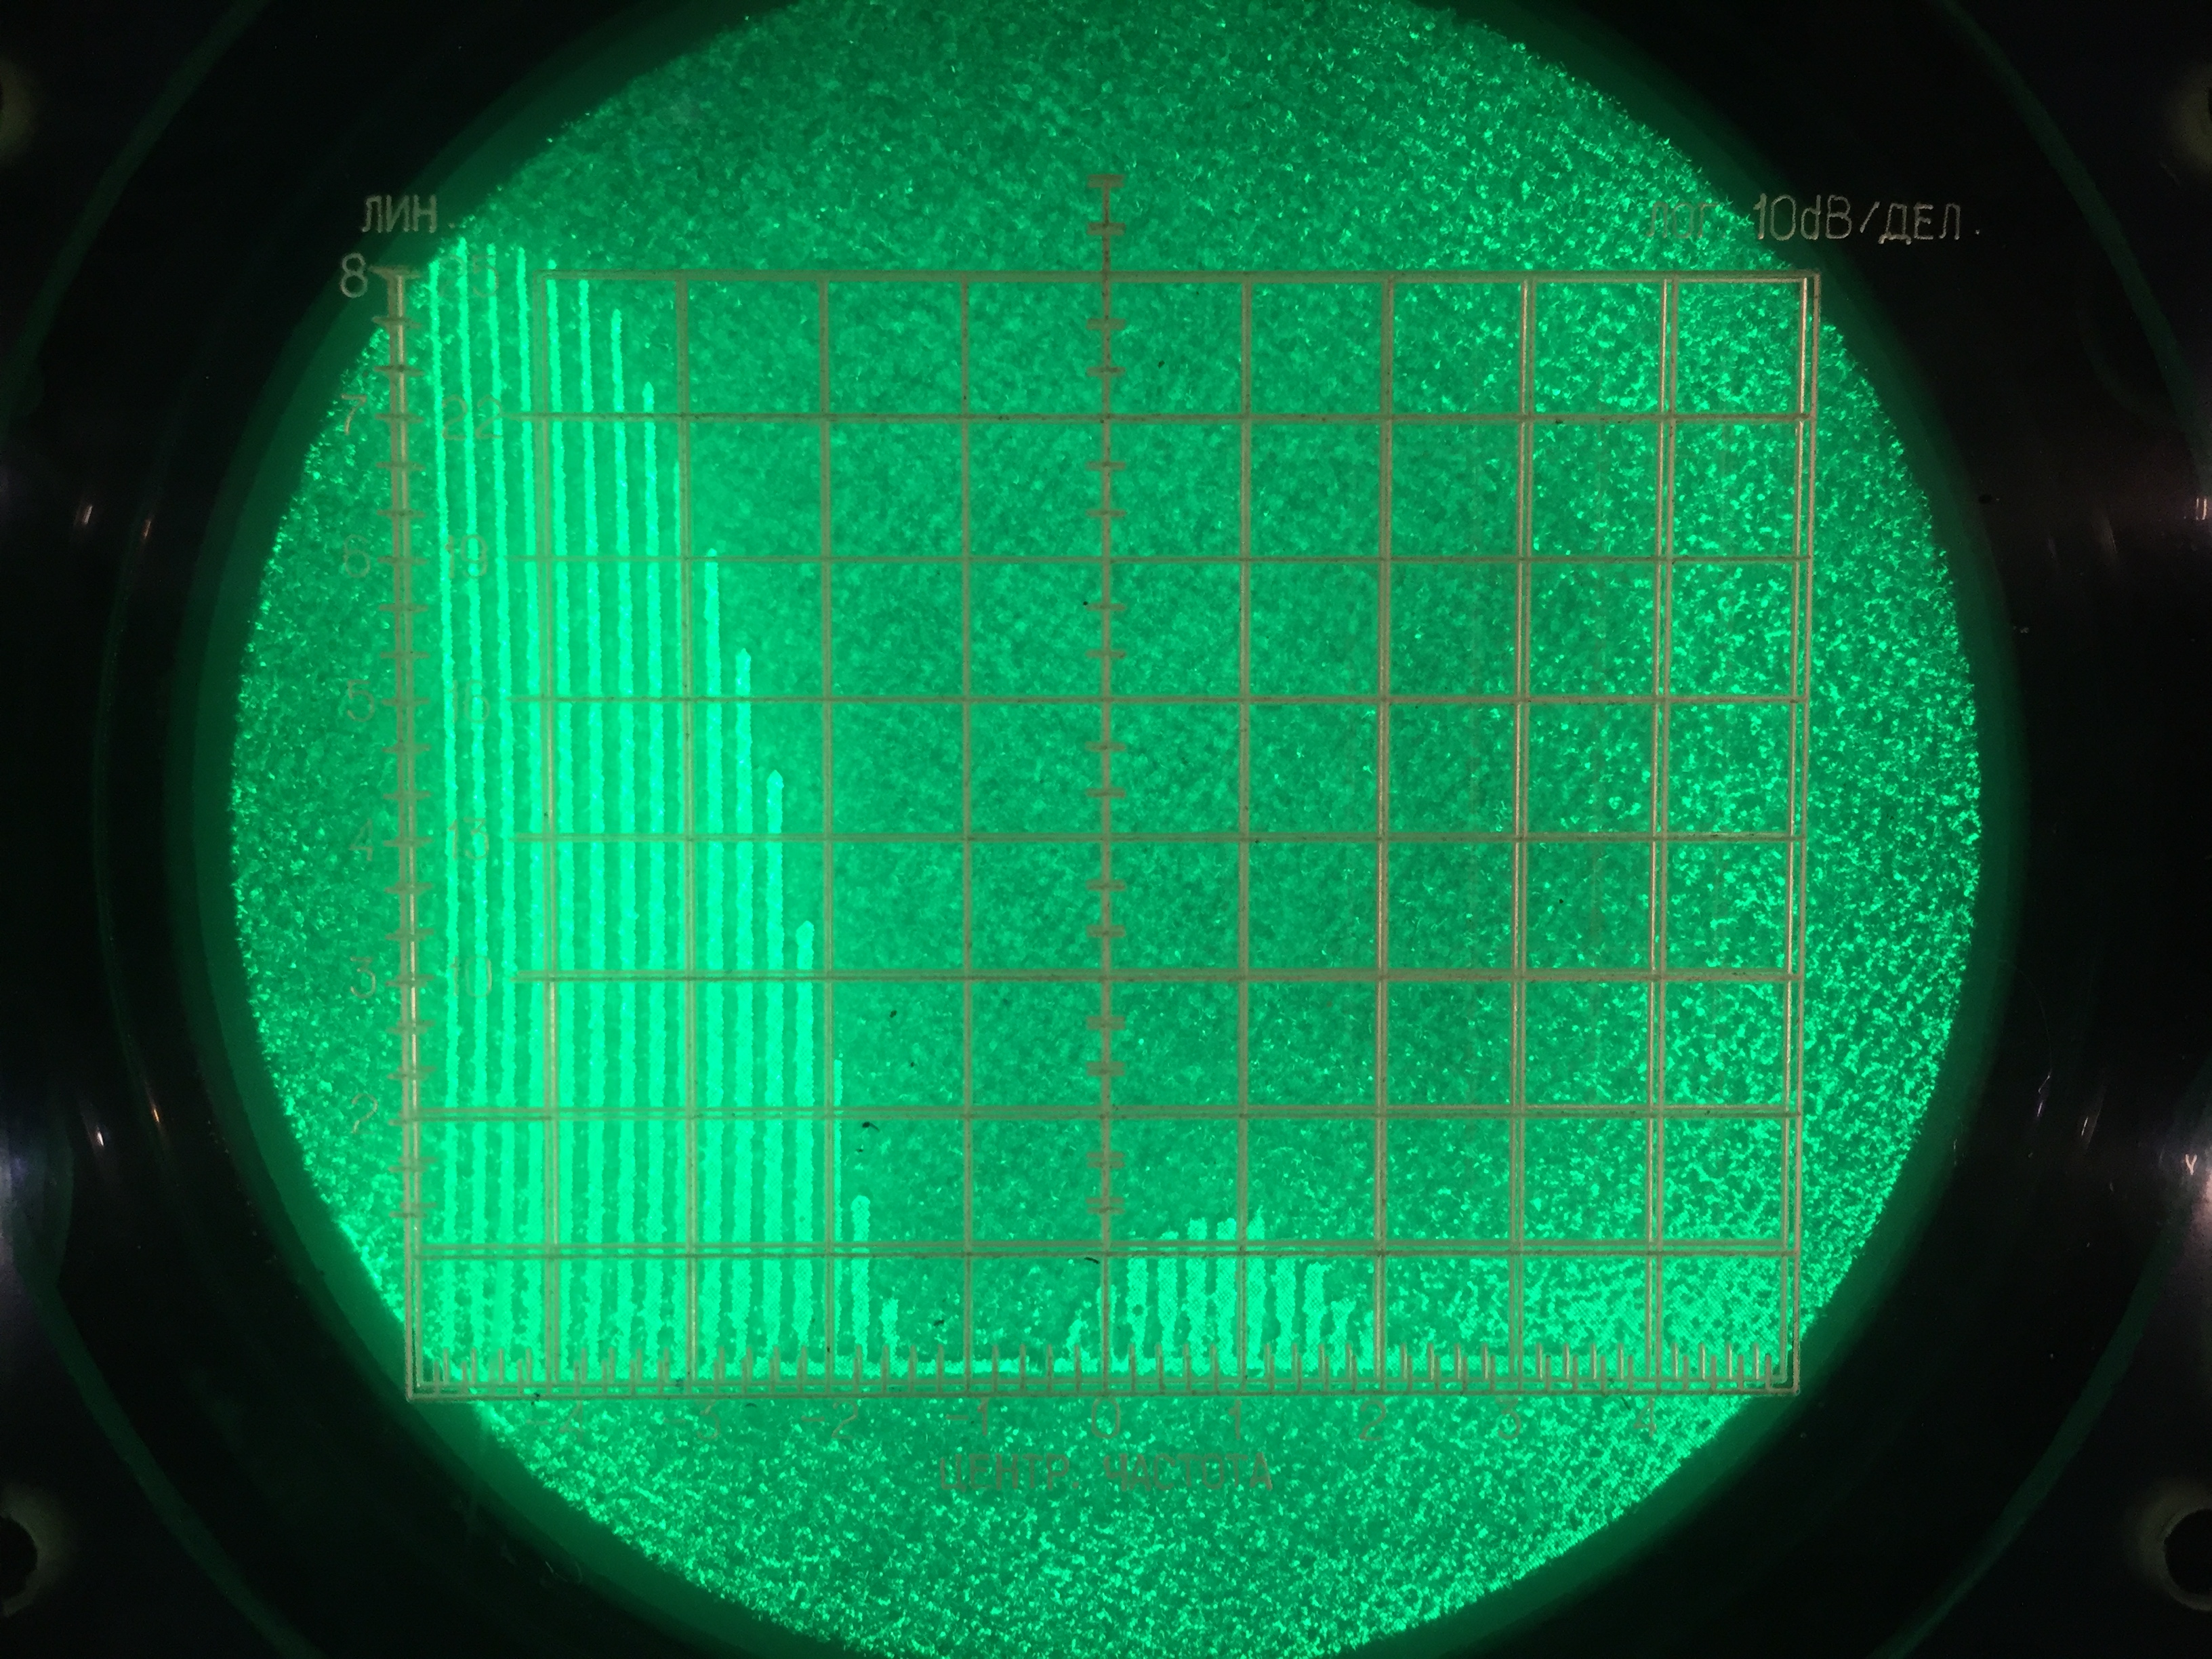
\includegraphics[width=0.9\linewidth]{IMG_0623} \\ $f_{\text{повт}}=1\text{кГц}$ \\ $ \tau = 50 \text{мкс}$}
	\end{minipage}
	\begin{minipage}[h]{0.30\linewidth}
		\centering{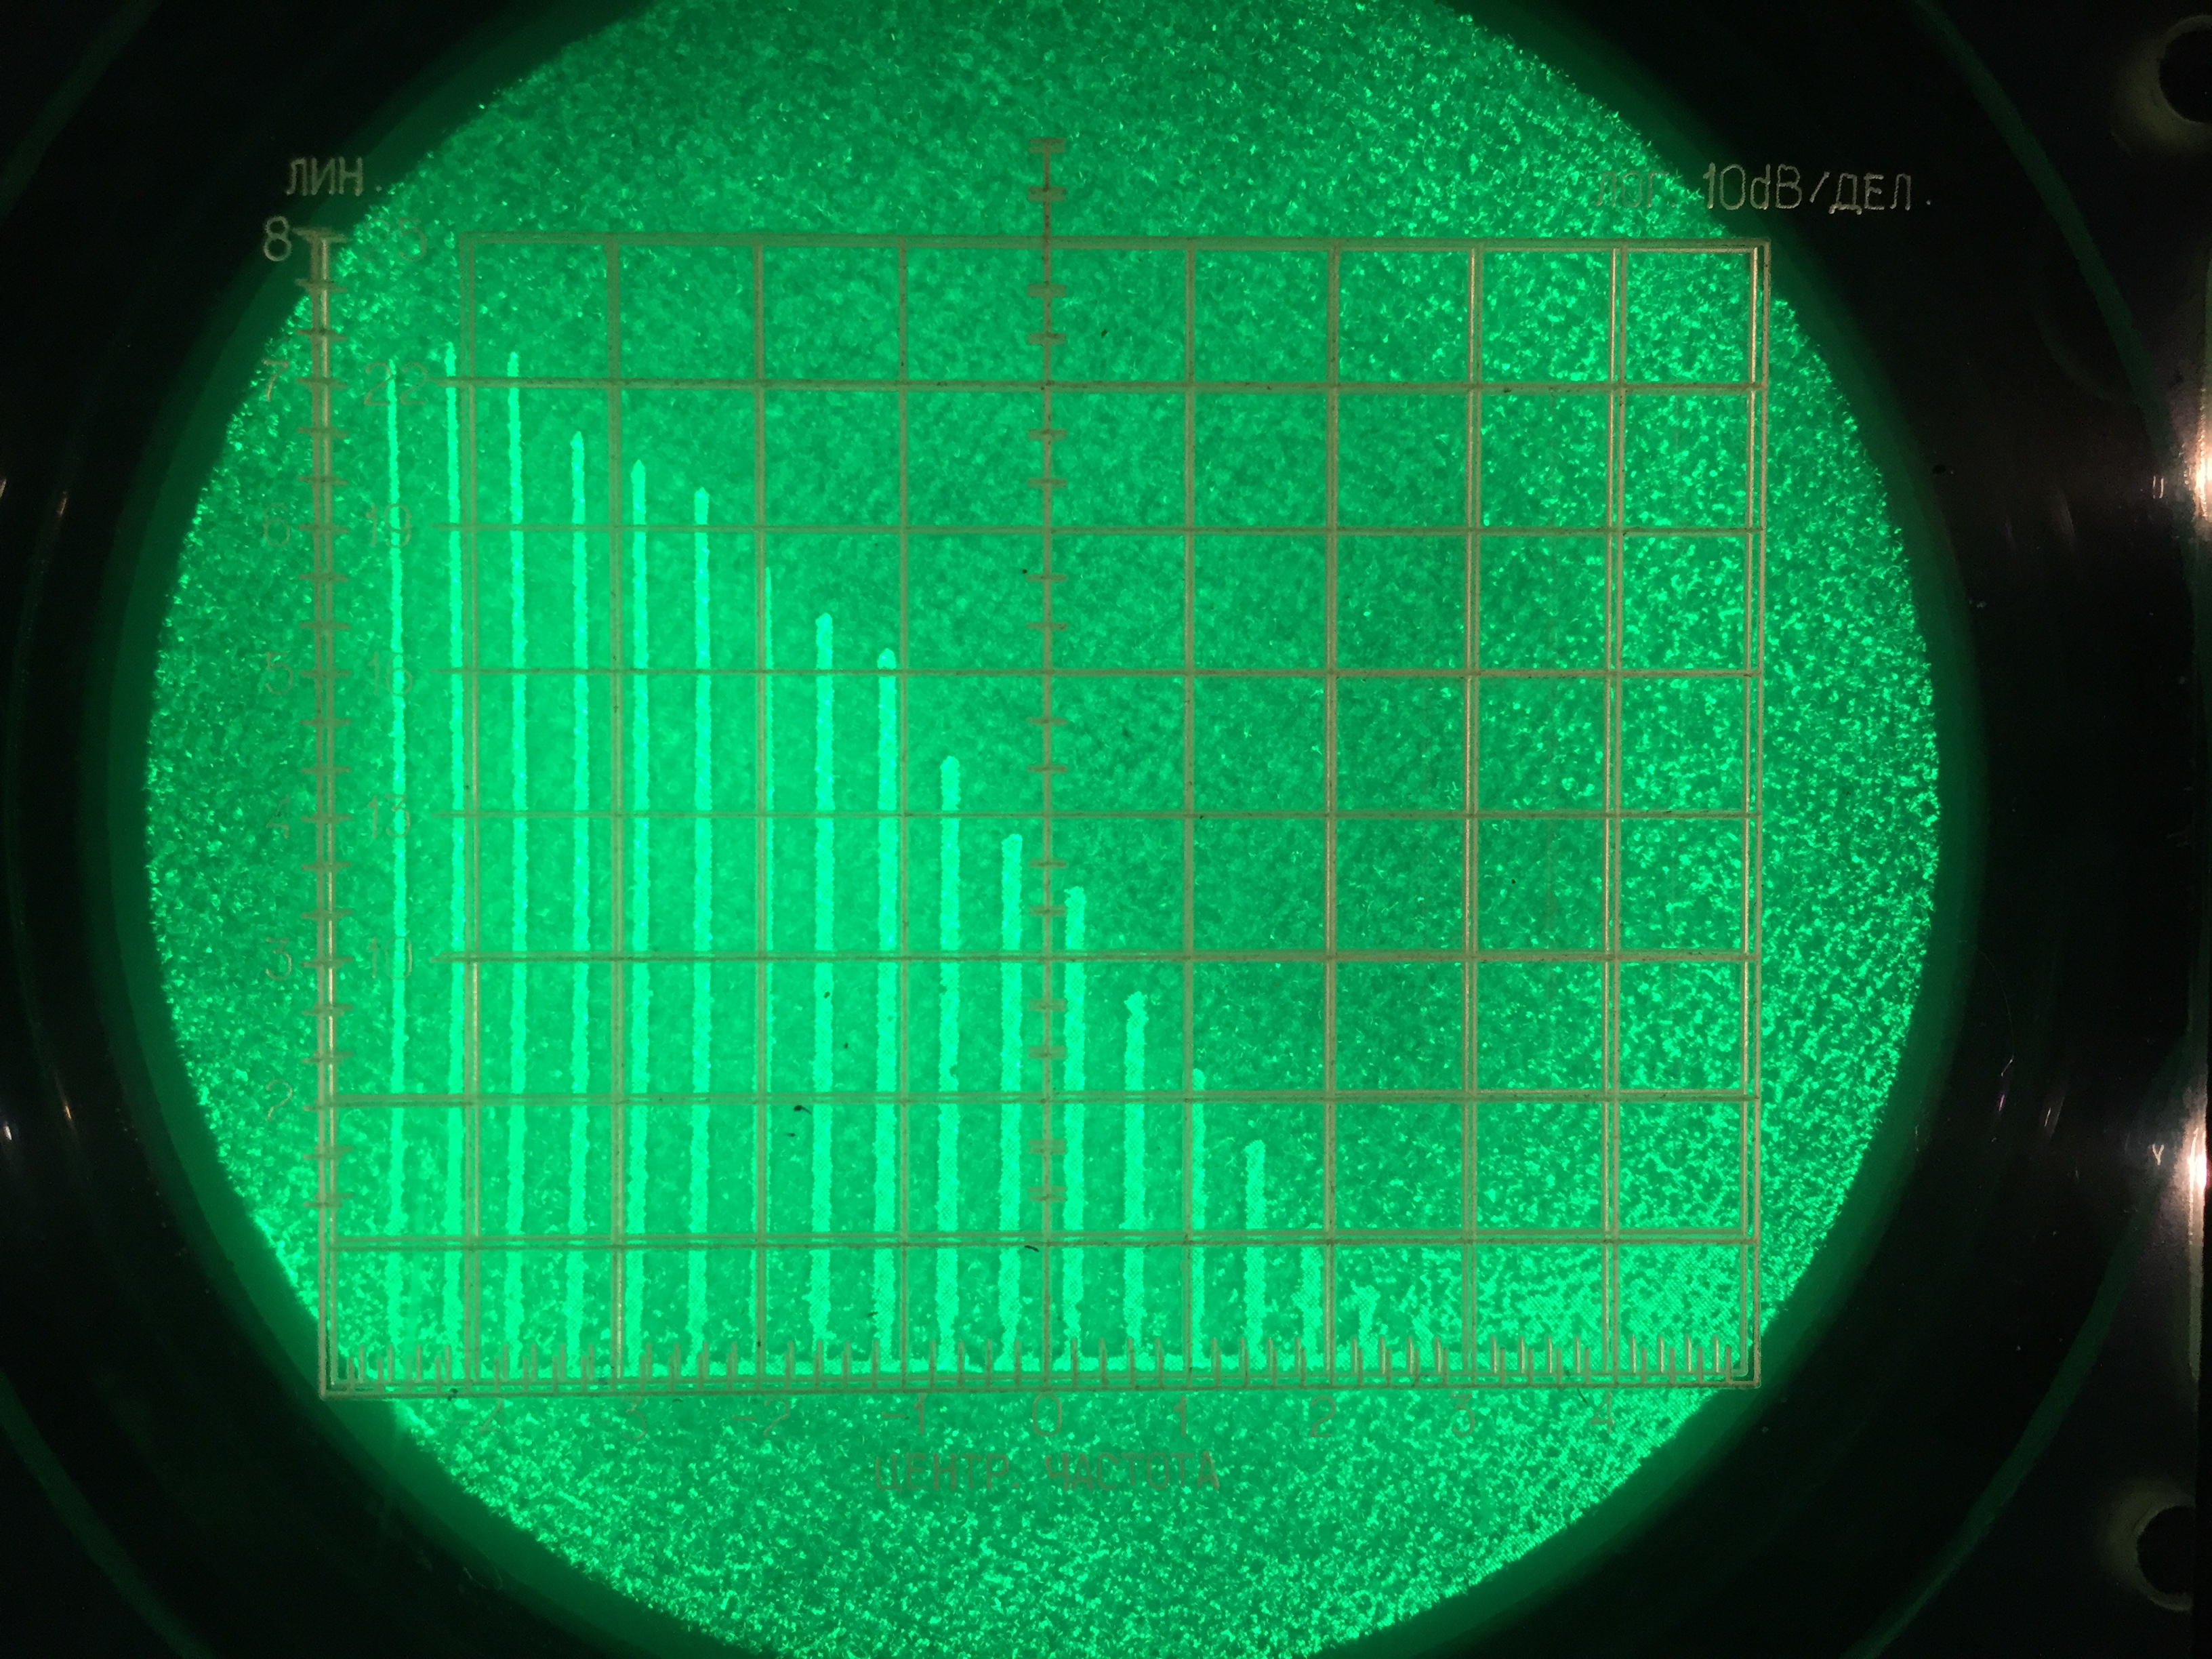
\includegraphics[width=0.9\linewidth]{IMG_0624} \\ $f_{\text{повт}}=2\text{кГц}$ \\ $ \tau = 25 \text{мкс}$}
	\end{minipage}
	
	\caption{Зависимость спектра от длительности $\tau$ и частоты $f_{\text{повт}}$.}
	\label{ris:image1}
\end{figure}


При увеличении $\tau$ вдвое при неизменной частоте повторений, уменьшается ширина спектра $\Delta \nu $. При увеличении частоты повторений $f_\text{повт}$ вдвое при неизменном $\tau$, увеличивается расстояние $\delta \nu$. 

\subsubsection*{Измерение зависимости ширины спектра от длительности импульса $\Delta\nu(\tau)$.}

\begin{table}[H]
\centering
\caption{Зависимость ширины $\Delta \nu$ спектра  от длительности импульса $\tau$}

\begin{tabular}{|c|c|c|c|c|c|c|c|c|}
\hline
$\tau, \text{мкс}$       & 25   & 50   & 75   & 100   & 125   & 150 & 175 & 200 \\ \hline 
$\Delta \nu, \text{кГц}$ & 31  & 14   & 8   & 7   & 7   & 5 & 4 & 4        \\ \hline
$1/\tau, \text{кГц}$     & 40   & 20   & 13,3 & 10 & 8 & 6,7 & 5,7 &5          \\ \hline
\end{tabular}


\end{table}

\begin{figure}[H]
\centering
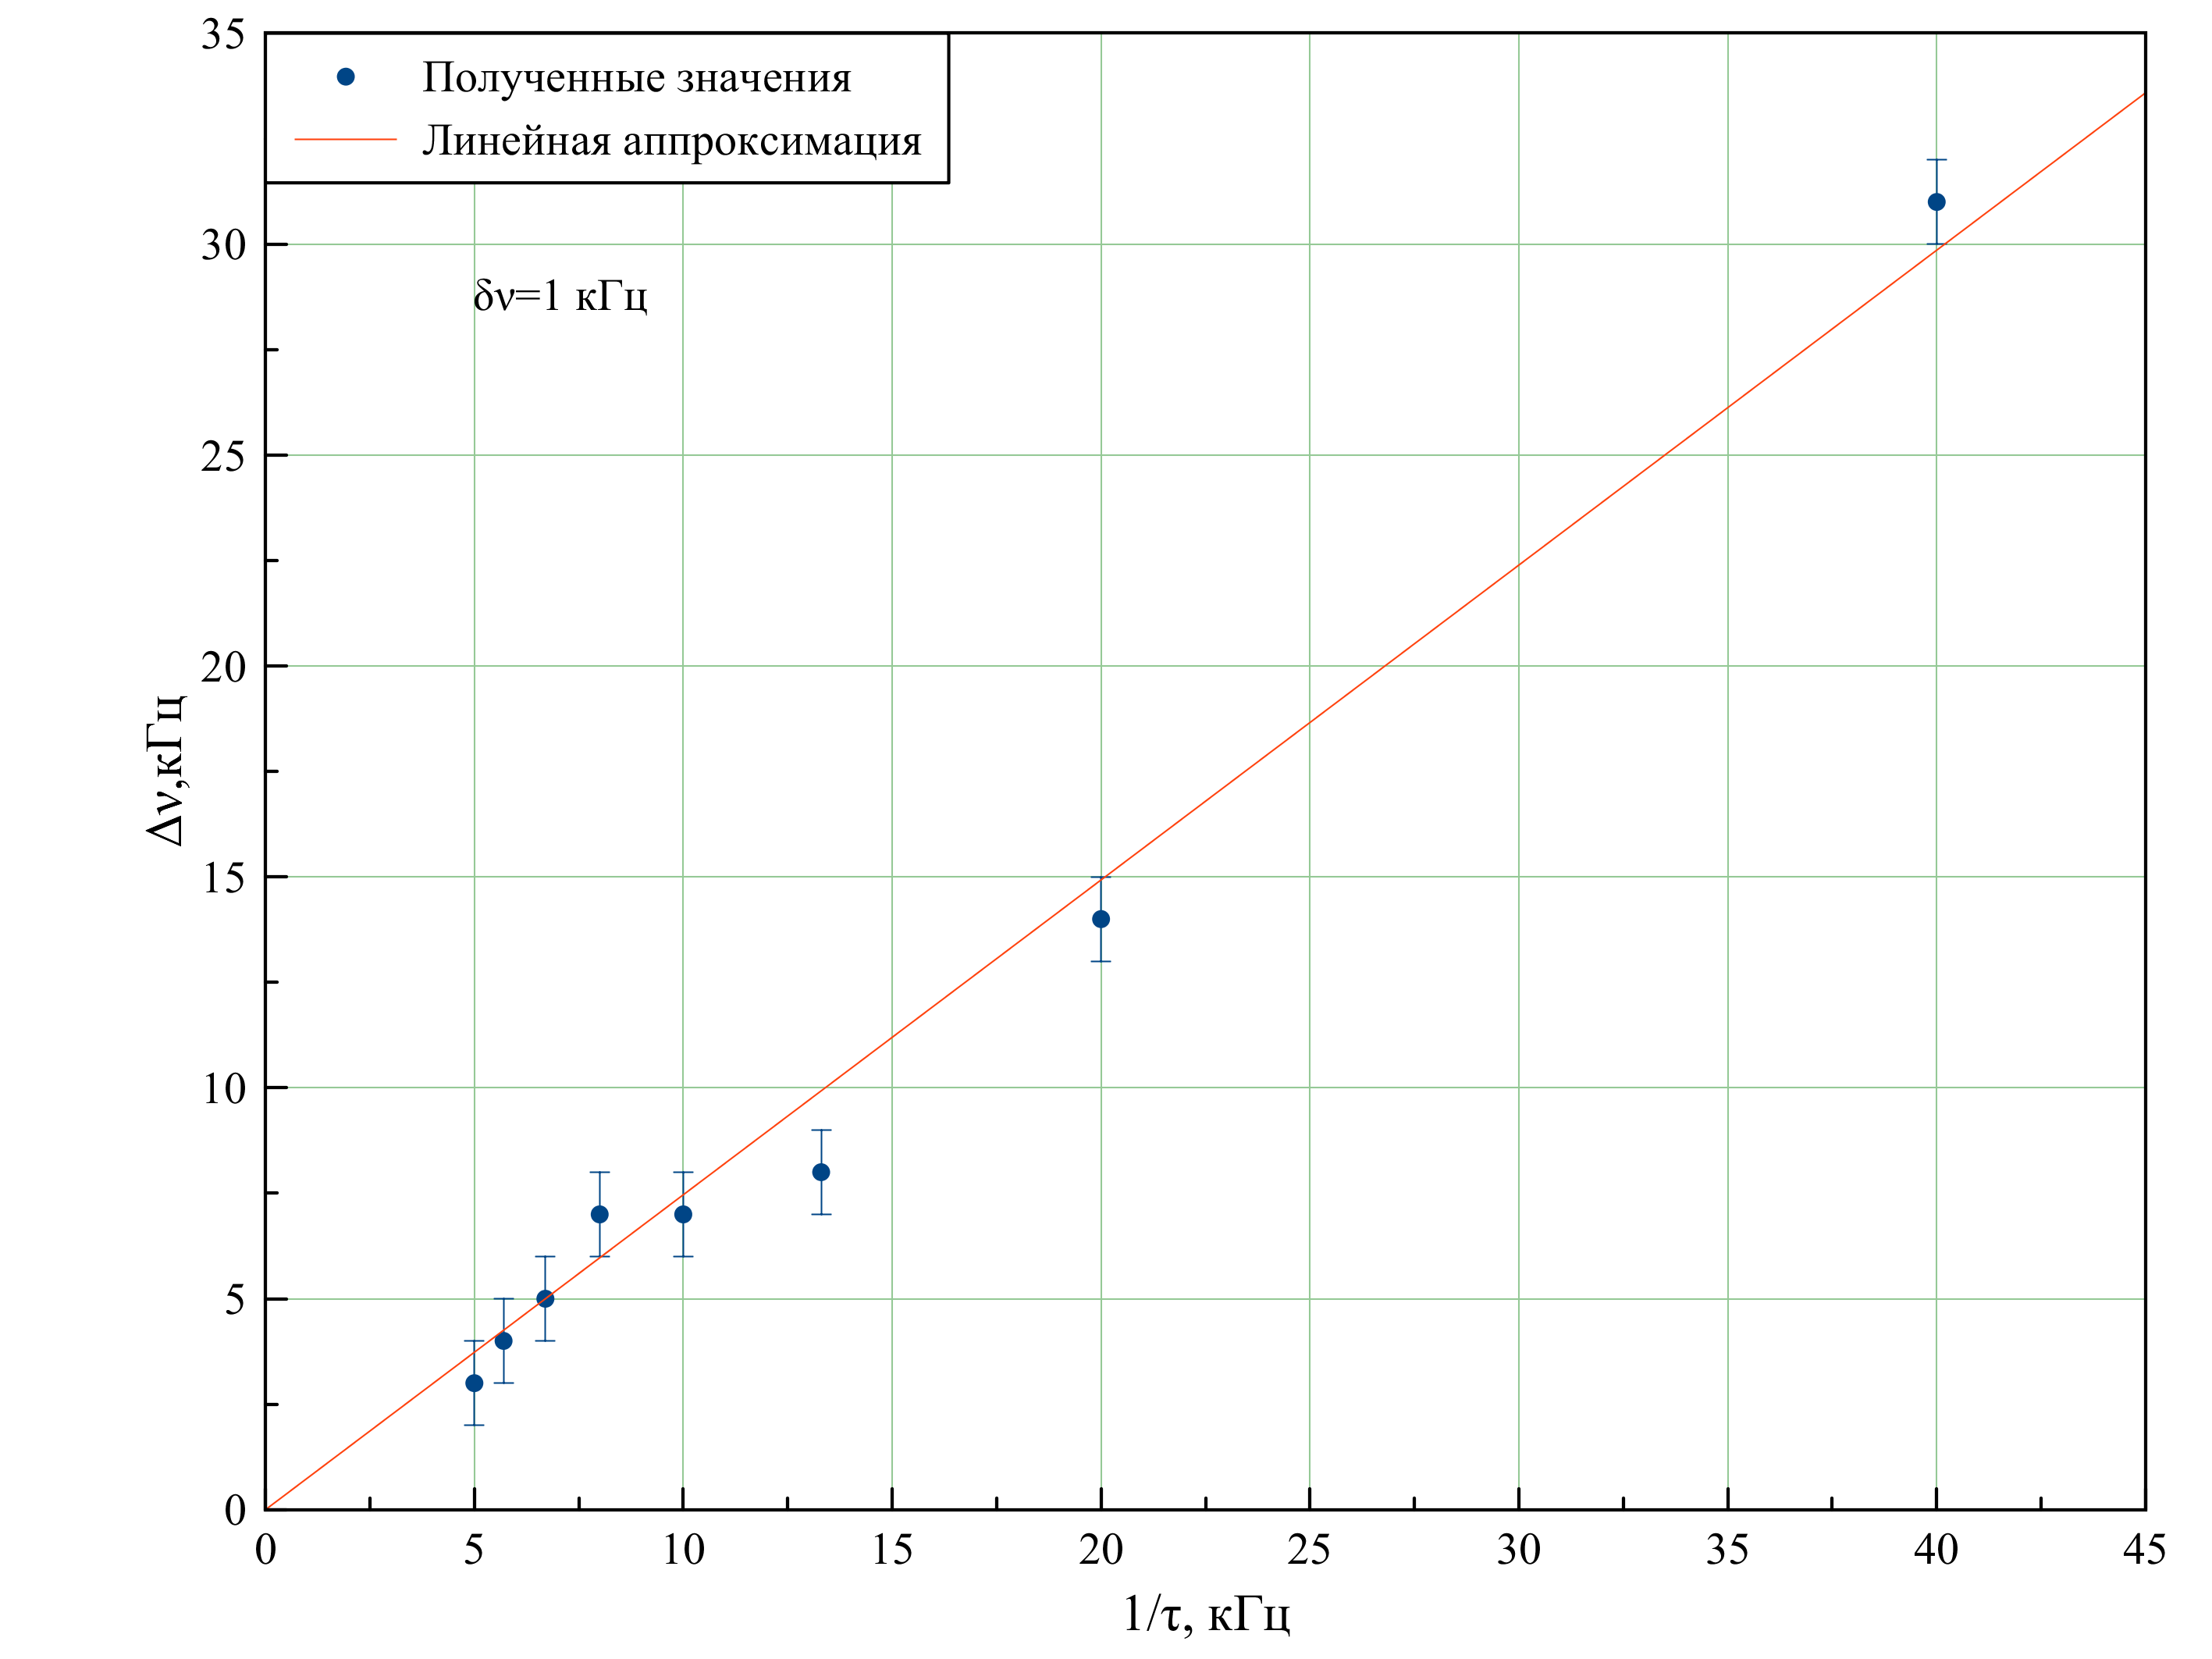
\includegraphics[width = 0.95\textwidth]{graphic10}
\caption{График зависимости $\Delta \nu (\frac{1}{\tau})$}
\end{figure}

Коэффициент угла наклона прямой и его погрешность посчитаем методом наименьших квадратов(точку с координатами (13,3;8) учитывать не будем): $k = \langle \Delta \nu \tau \rangle \cdot \langle \tau^2 \rangle$, $\sigma_k = \dfrac{1}{\sqrt{n}} \sqrt{\langle \Delta \nu^2 \rangle \cdot \langle \tau^2 \rangle - k^2}$, тогда 
\begin{equation}
\fbox{$\Delta \nu \tau = 0.76 \pm 0.02 (\varepsilon \simeq 3\%)$}
\end{equation}

\begin{figure}[h]
	\centering
	\begin{minipage}[h]{0.49\linewidth}
		\centering{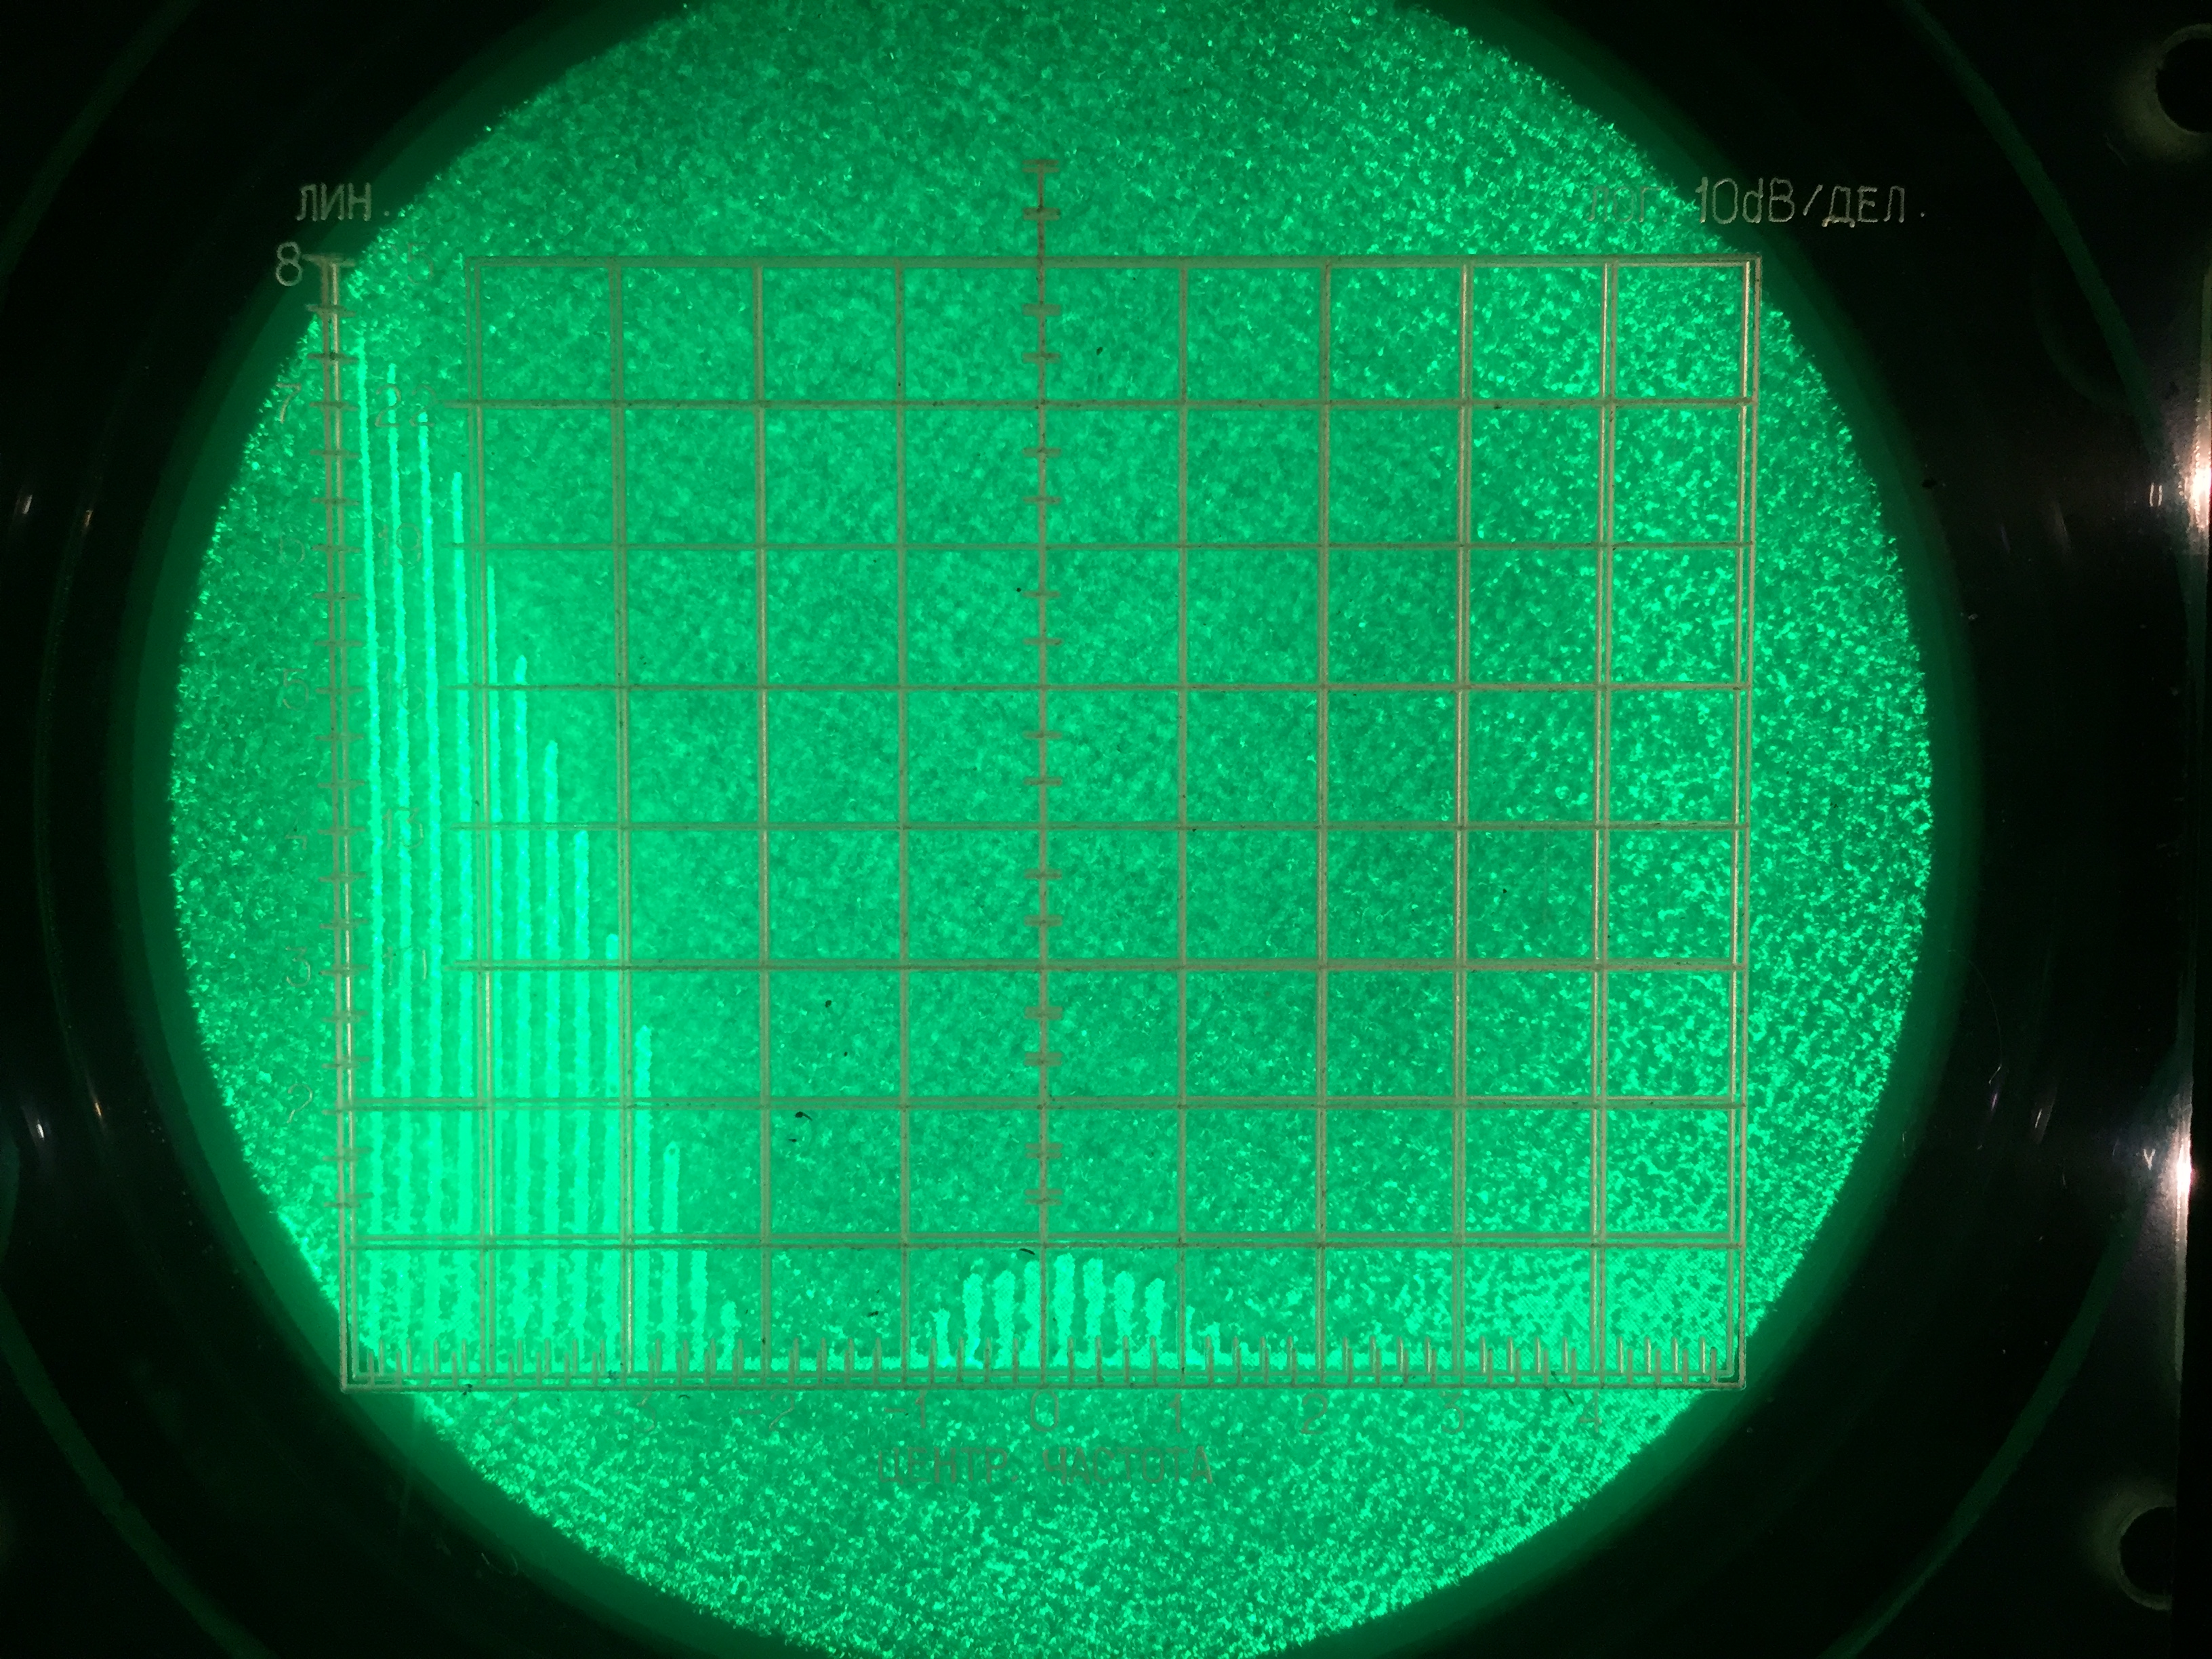
\includegraphics[width=0.9\linewidth]{IMG_0637} \\ $ \tau = 50 \text{мкс}$}
	\end{minipage}
	\begin{minipage}[h]{0.49\linewidth}
		\centering{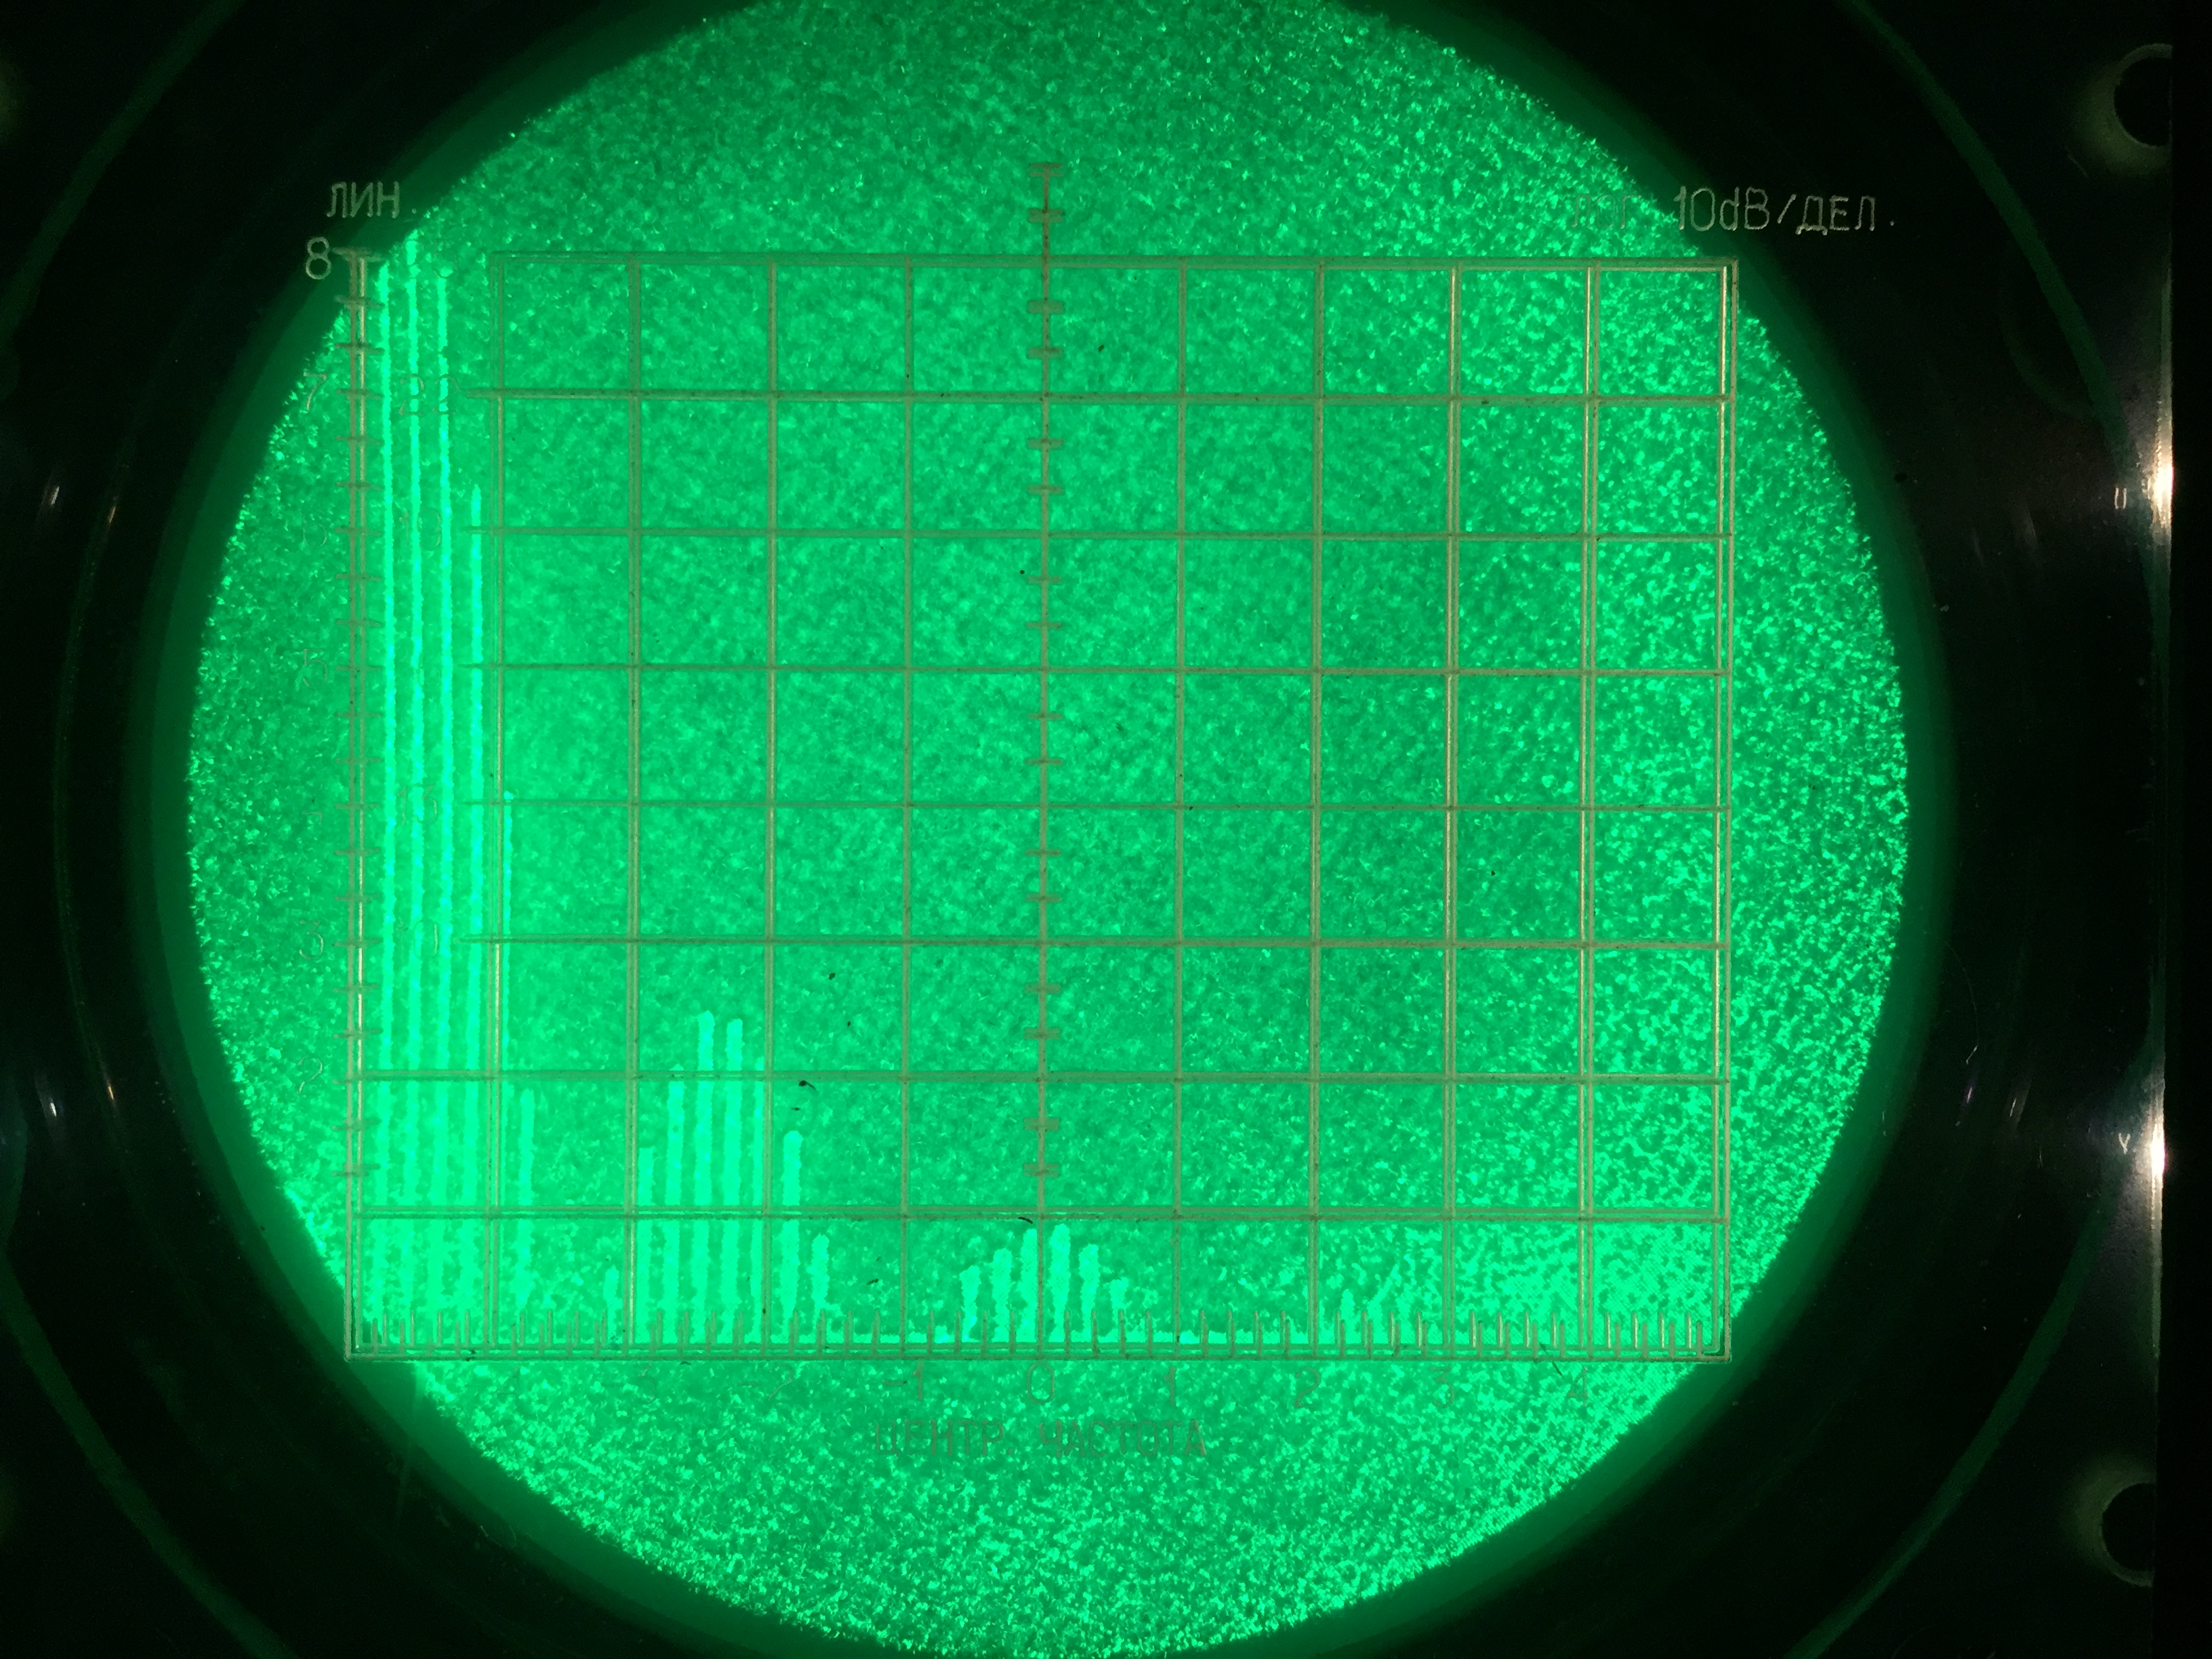
\includegraphics[width=0.9\linewidth]{IMG_0638} \\ $ \tau = 100 \text{мкс}$}
	\end{minipage}
	
	\caption{Зависимость спектра от длительности $\tau$ при частоте $f_{\text{повт}} = 1\text{кГц}$.}
	\label{ris:image1}
\end{figure}

\subsection*{Исследование спектра периодической последовательности цугов \\ гармонических колебаний}

Рассмотрим периодическую последовательность {\it{цугов}} (отдельных кусков синусоиды) гармонического колебания
$V_0 \cos (\omega_0 t)$ c длительностью цуга $\tau$ и периодом повторения $T$.
Тогда согласно \ref{form:a_n}:

\begin{equation}
\label{form:cug_a_n}
a_n = \frac{2}{T}\int\limits_{ -\frac{\tau}{2} } ^ {\frac{\tau}{2} } V_0\cos(\omega_0t)\cdot \cos(n\Omega_1)\, dt
\end{equation}

Сравнивания спектр последовательности прямоугольных импульсов и спектр цугов, мы видим, что они аналогичны, но их максимумы сдвинуты по частоте на величину $\omega_{0}$.

\subsubsection*{Выполнение}

В работе используются: \textit{анализатор спектра СК4-56; генератор прямоугольных импульсов Г5-54; осциллограф; генератор сигналов Г6-34}

\begin{figure}[H]
\centering
\includegraphics[width = 0.8\textwidth]{schemeB}
\caption{Схема для исследования спектра периодической последовательности цугов высокочастотных колебаний}
\label{img:scheme B}
\end{figure}

Собираем схему согласно \ref{img:scheme B}. Получаем на экране осциллографа последовательность периодических {\it{цугов}} гармонических колебаний, получаемых модулированием синусоиды прямоугольными импульсами. Подключаем анализатор спектра СК4-56 и после настройки наблюдаем спектр сигнала с параметрами: $$\nu_{0} = 25\text{кГц}, \tau = 50\text{мкс}, f_{\text{повт}} = 1\text{кГц}.$$




При увеличении $\tau$ вдвое при неизменной частоте повторений, вдвое уменьшается ширина спектра (рис.~\ref{ris:image1}), в соответствии с соотношением неопределенности: $\Delta \nu \tau \simeq 1$.



\begin{figure}[h]
	\centering
	\begin{minipage}[h]{0.49\linewidth}
		\centering{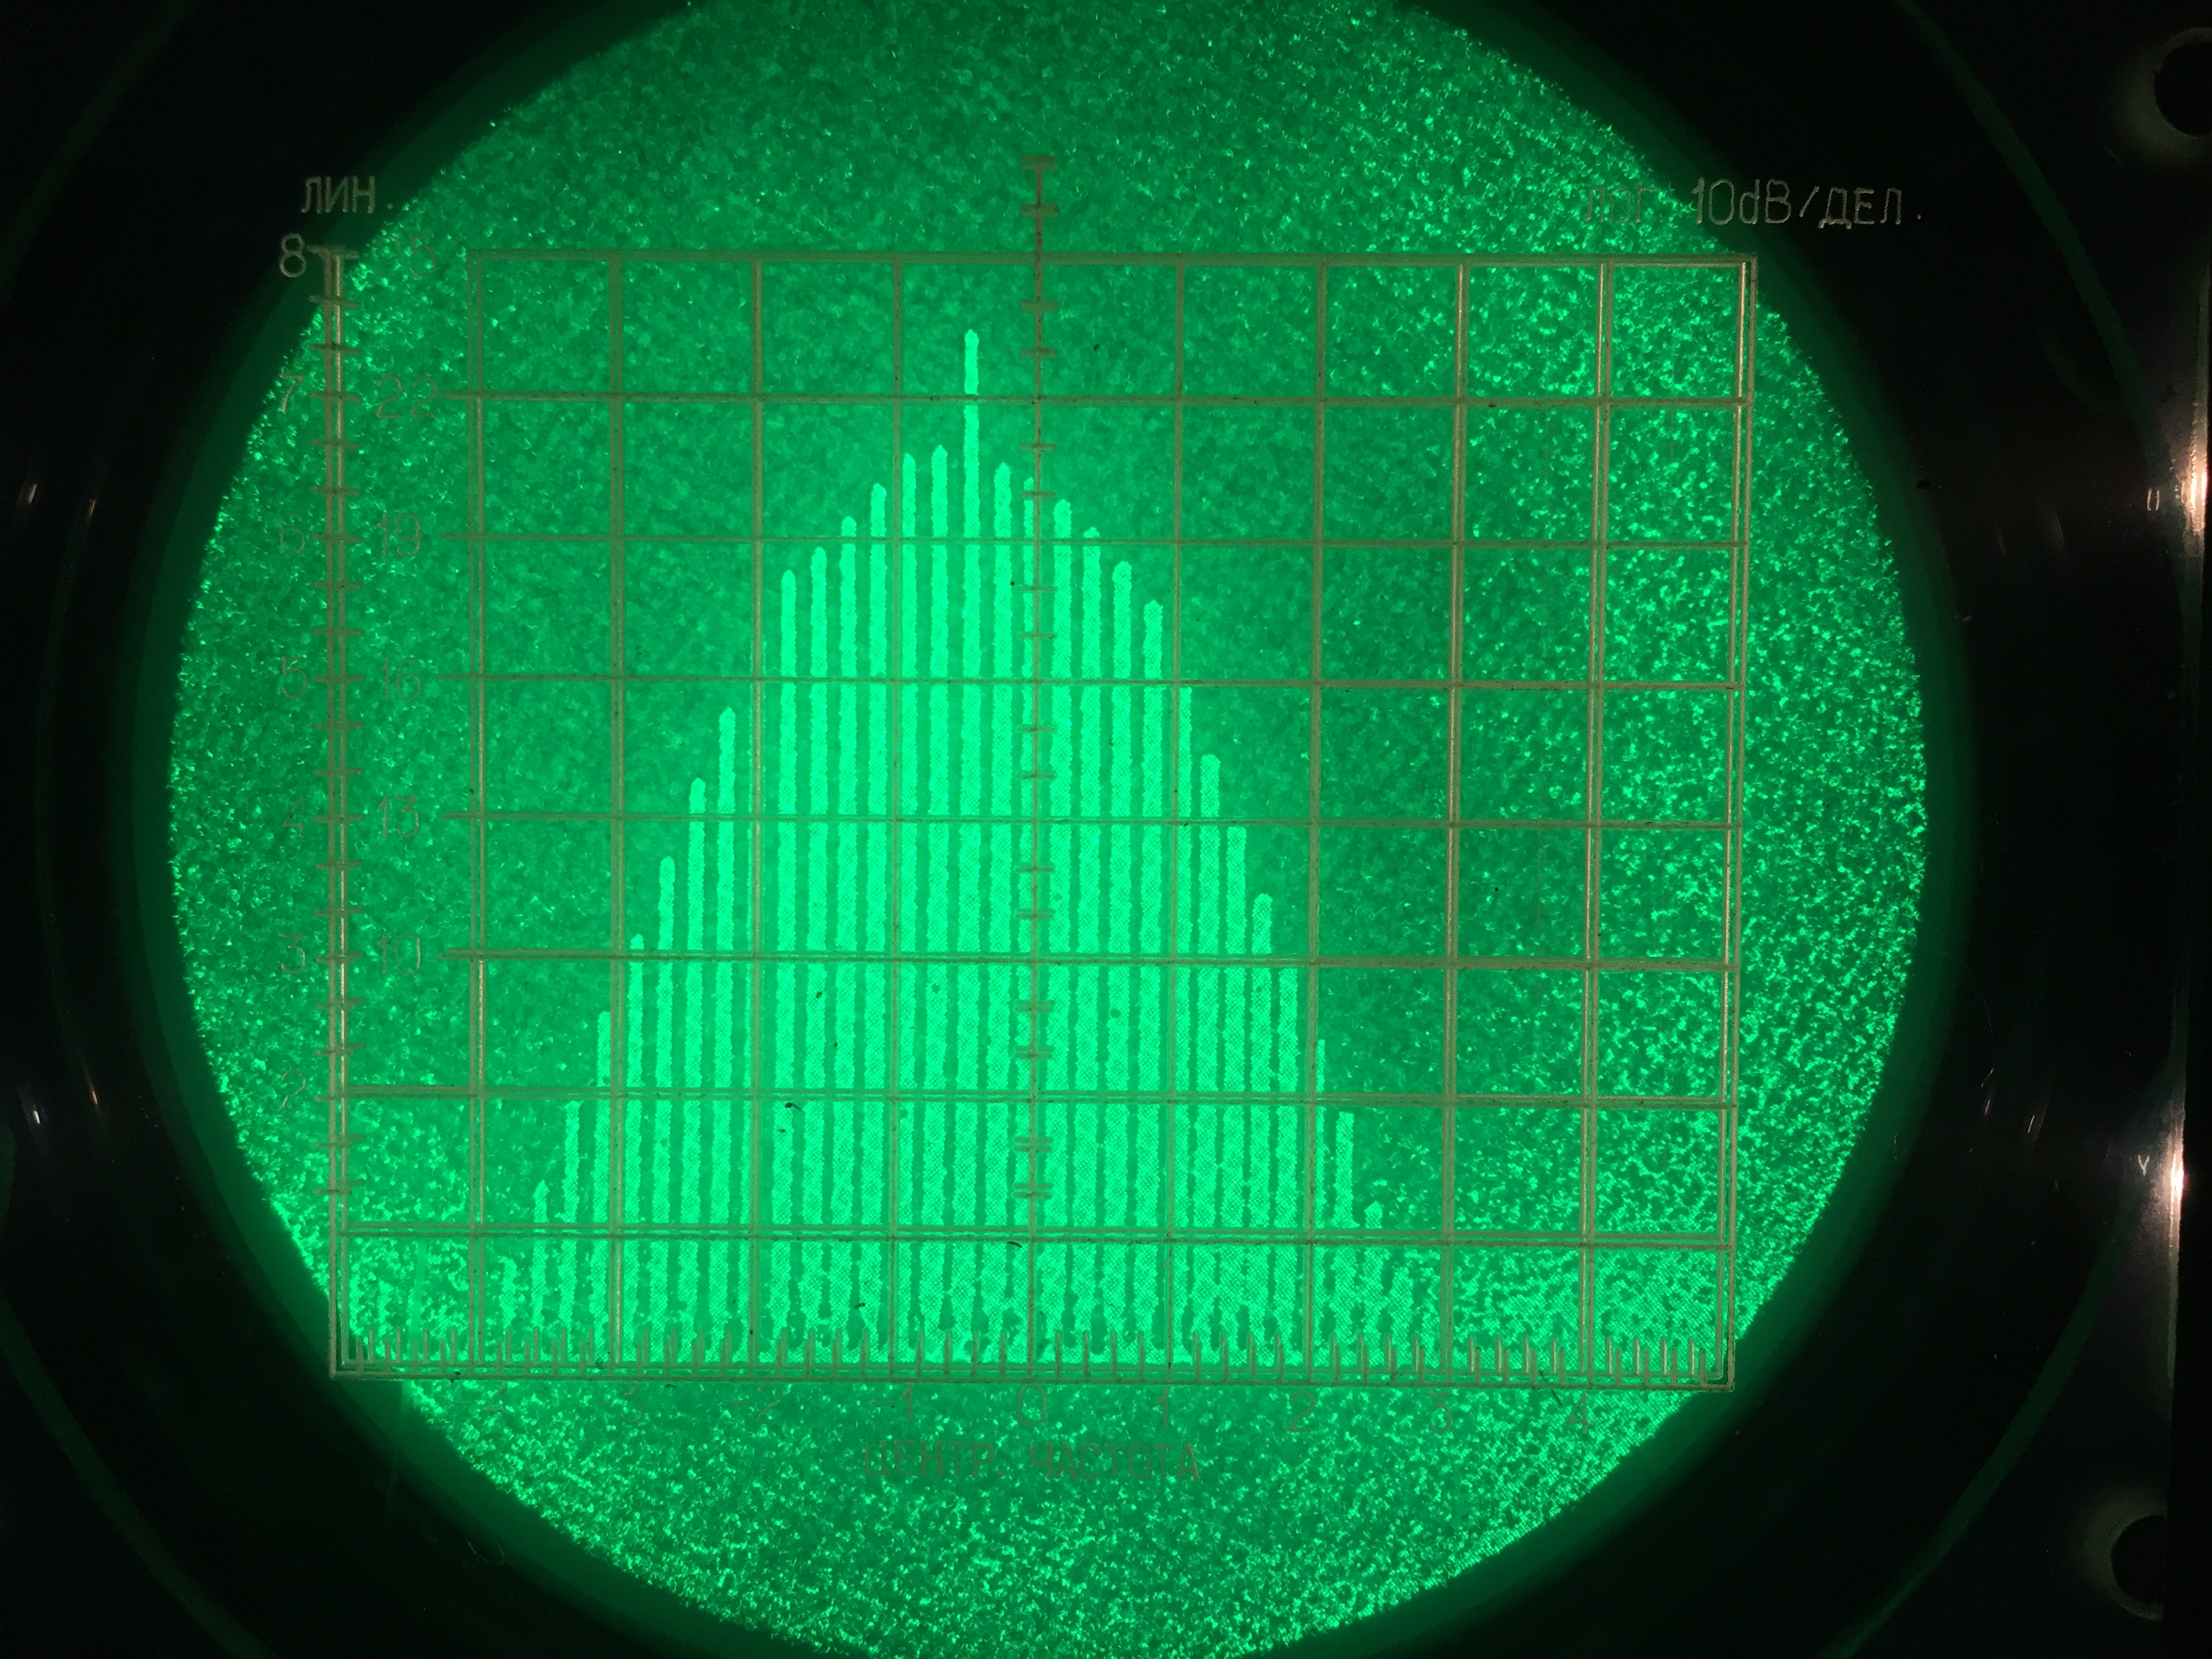
\includegraphics[width=0.9\linewidth]{IMG_0641} \\ а)$ \tau = 50 \text{мкс}$}
	\end{minipage}
	\begin{minipage}[h]{0.49\linewidth}
		\centering{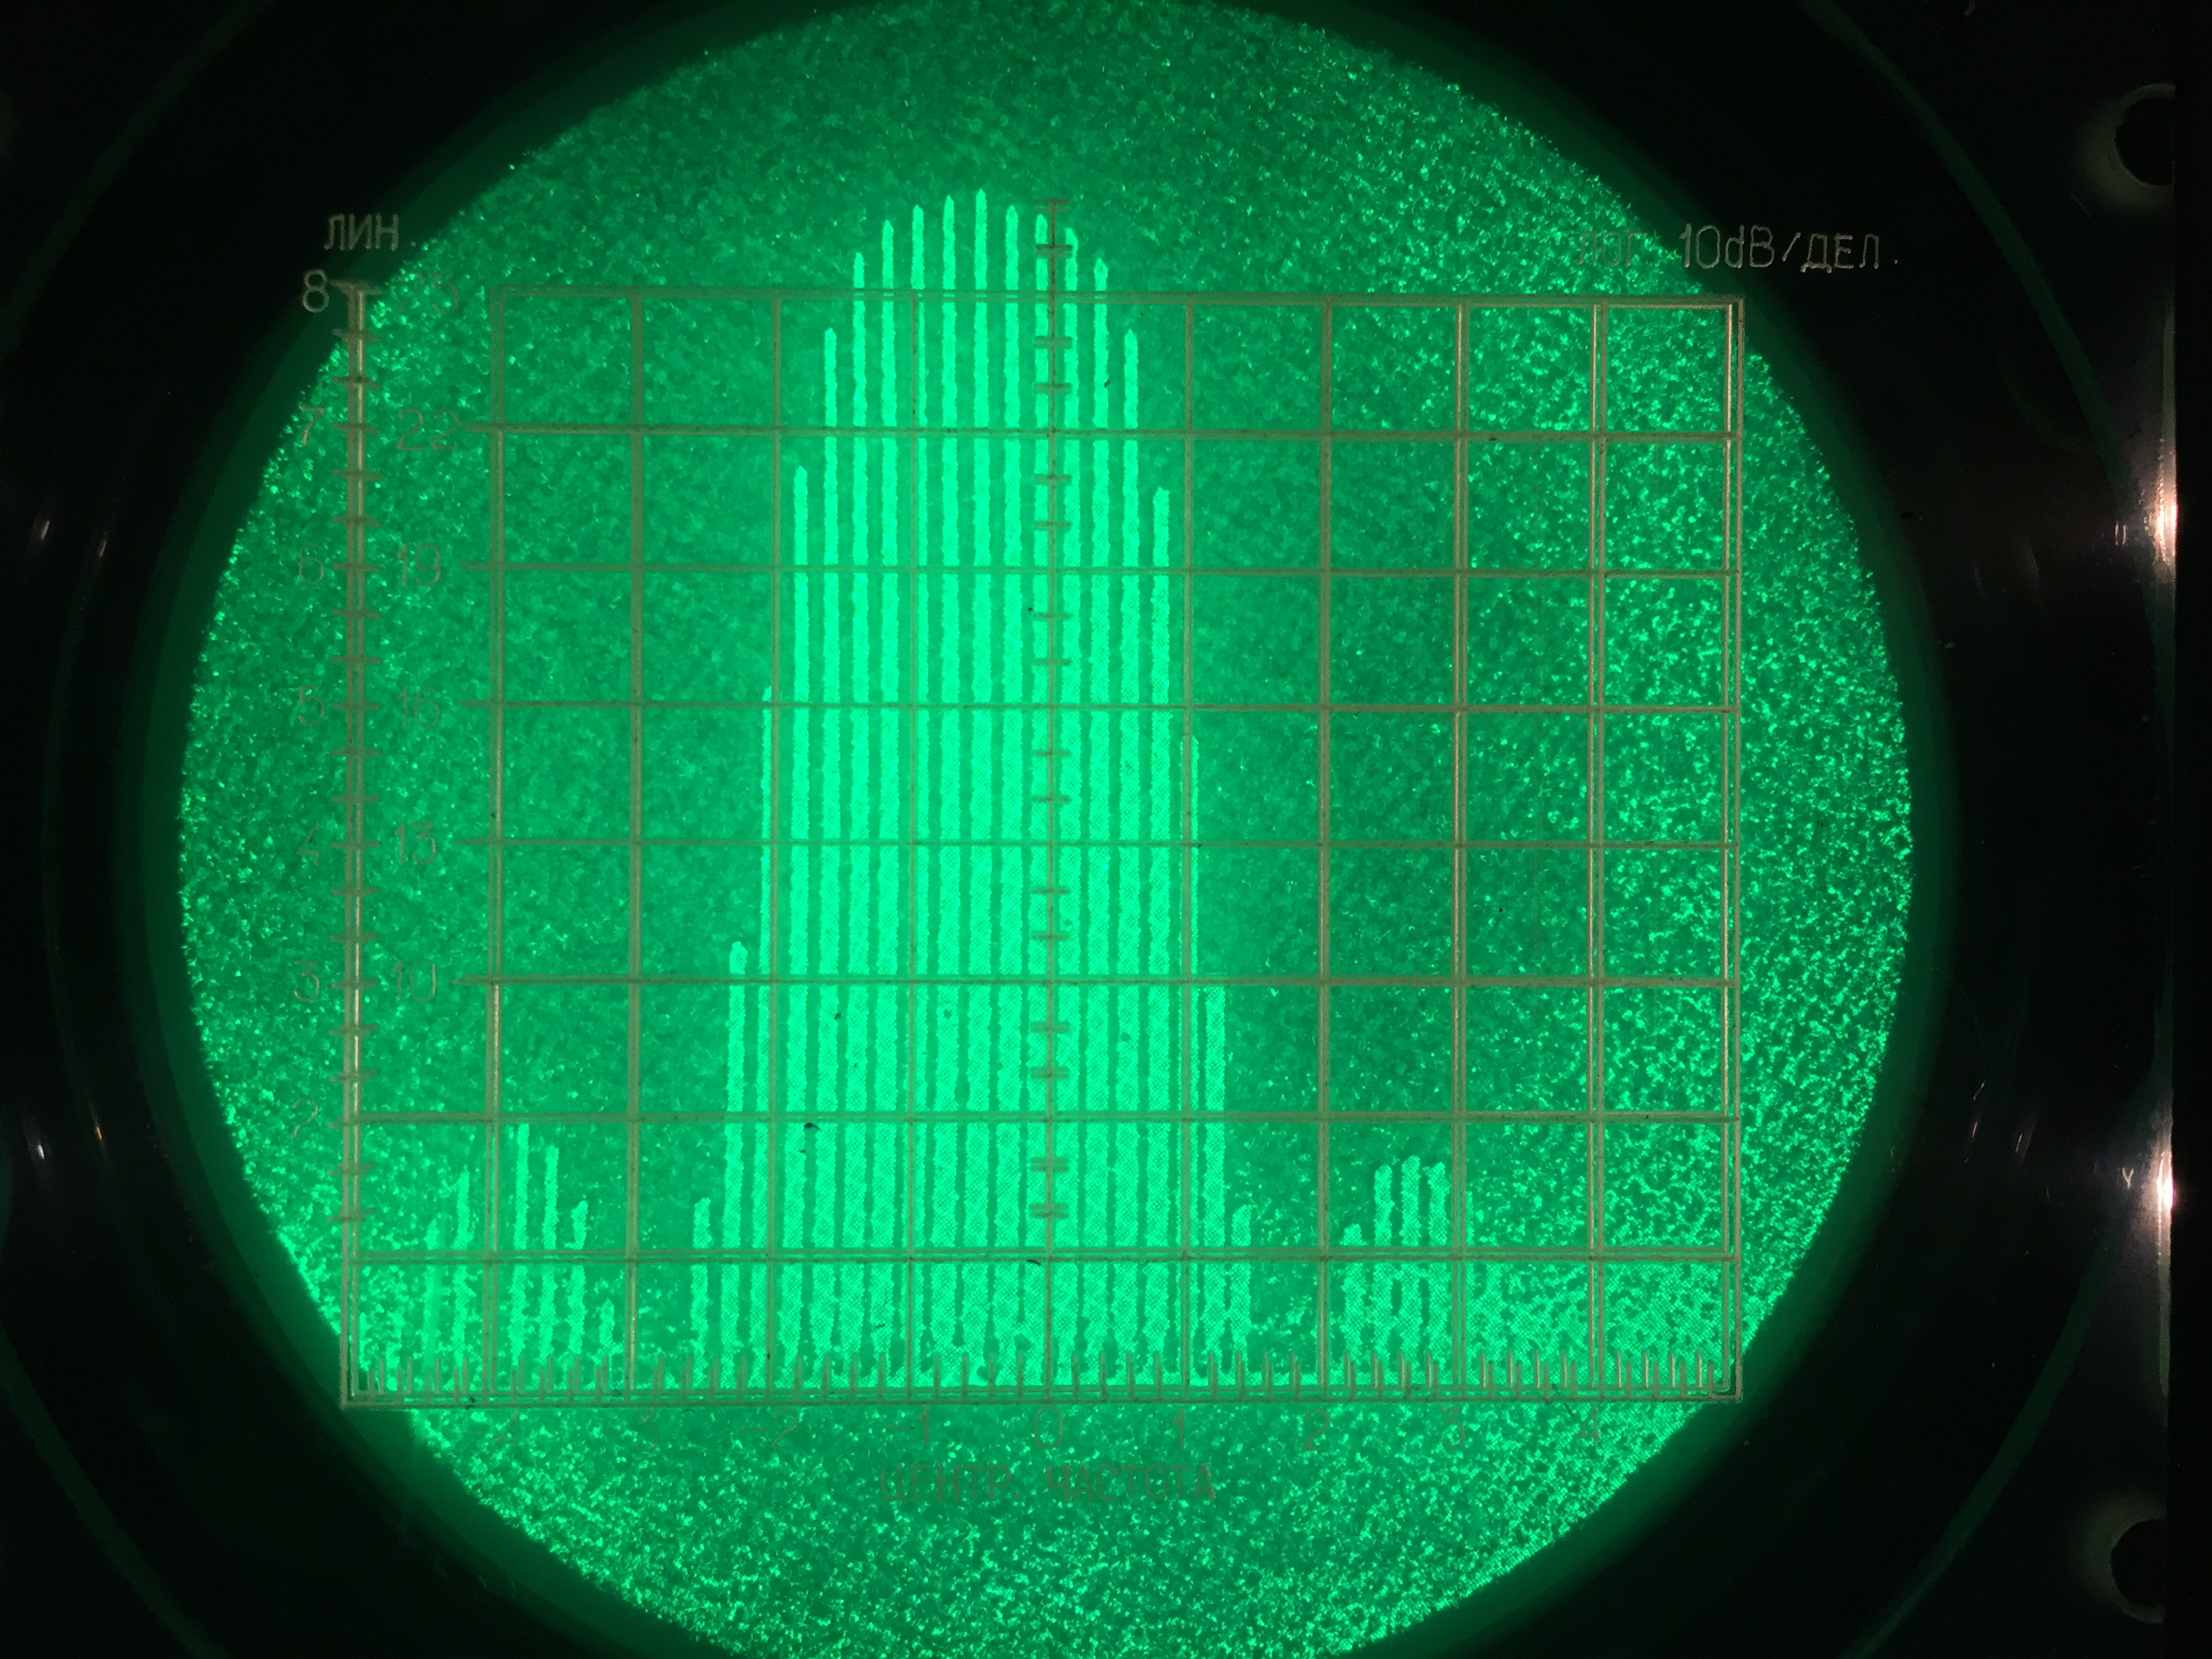
\includegraphics[width=0.9\linewidth]{IMG_0642} \\ б)$ \tau = 100 \text{мкс}$}
	\end{minipage}
	
	\caption{Зависимость спектра от длительности $\tau$ при частоте $f_{\text{повт}} = 1\text{кГц}$ и $\nu_{0} = 25\text{кГц}$.}
	\label{ris:image1}
\end{figure}



При изменении несущей частоты  $\nu_0 = 25, 10 \; \text{или} \; 40\; \text{кГц}$ при неизменных $f_\text{повт} = 10^3 \; \text{Гц}, \tau = 100 \; \text{мкс}, m_x = 5 \; \text{кГц}$, изменяется сдвиг спектра по оси частот(рис. \ref{ris:image1}(а) и рис. \ref{ris:image2}).


\begin{figure}[H]
	\centering
	
	\begin{minipage}[h]{0.49\linewidth}
		\centering{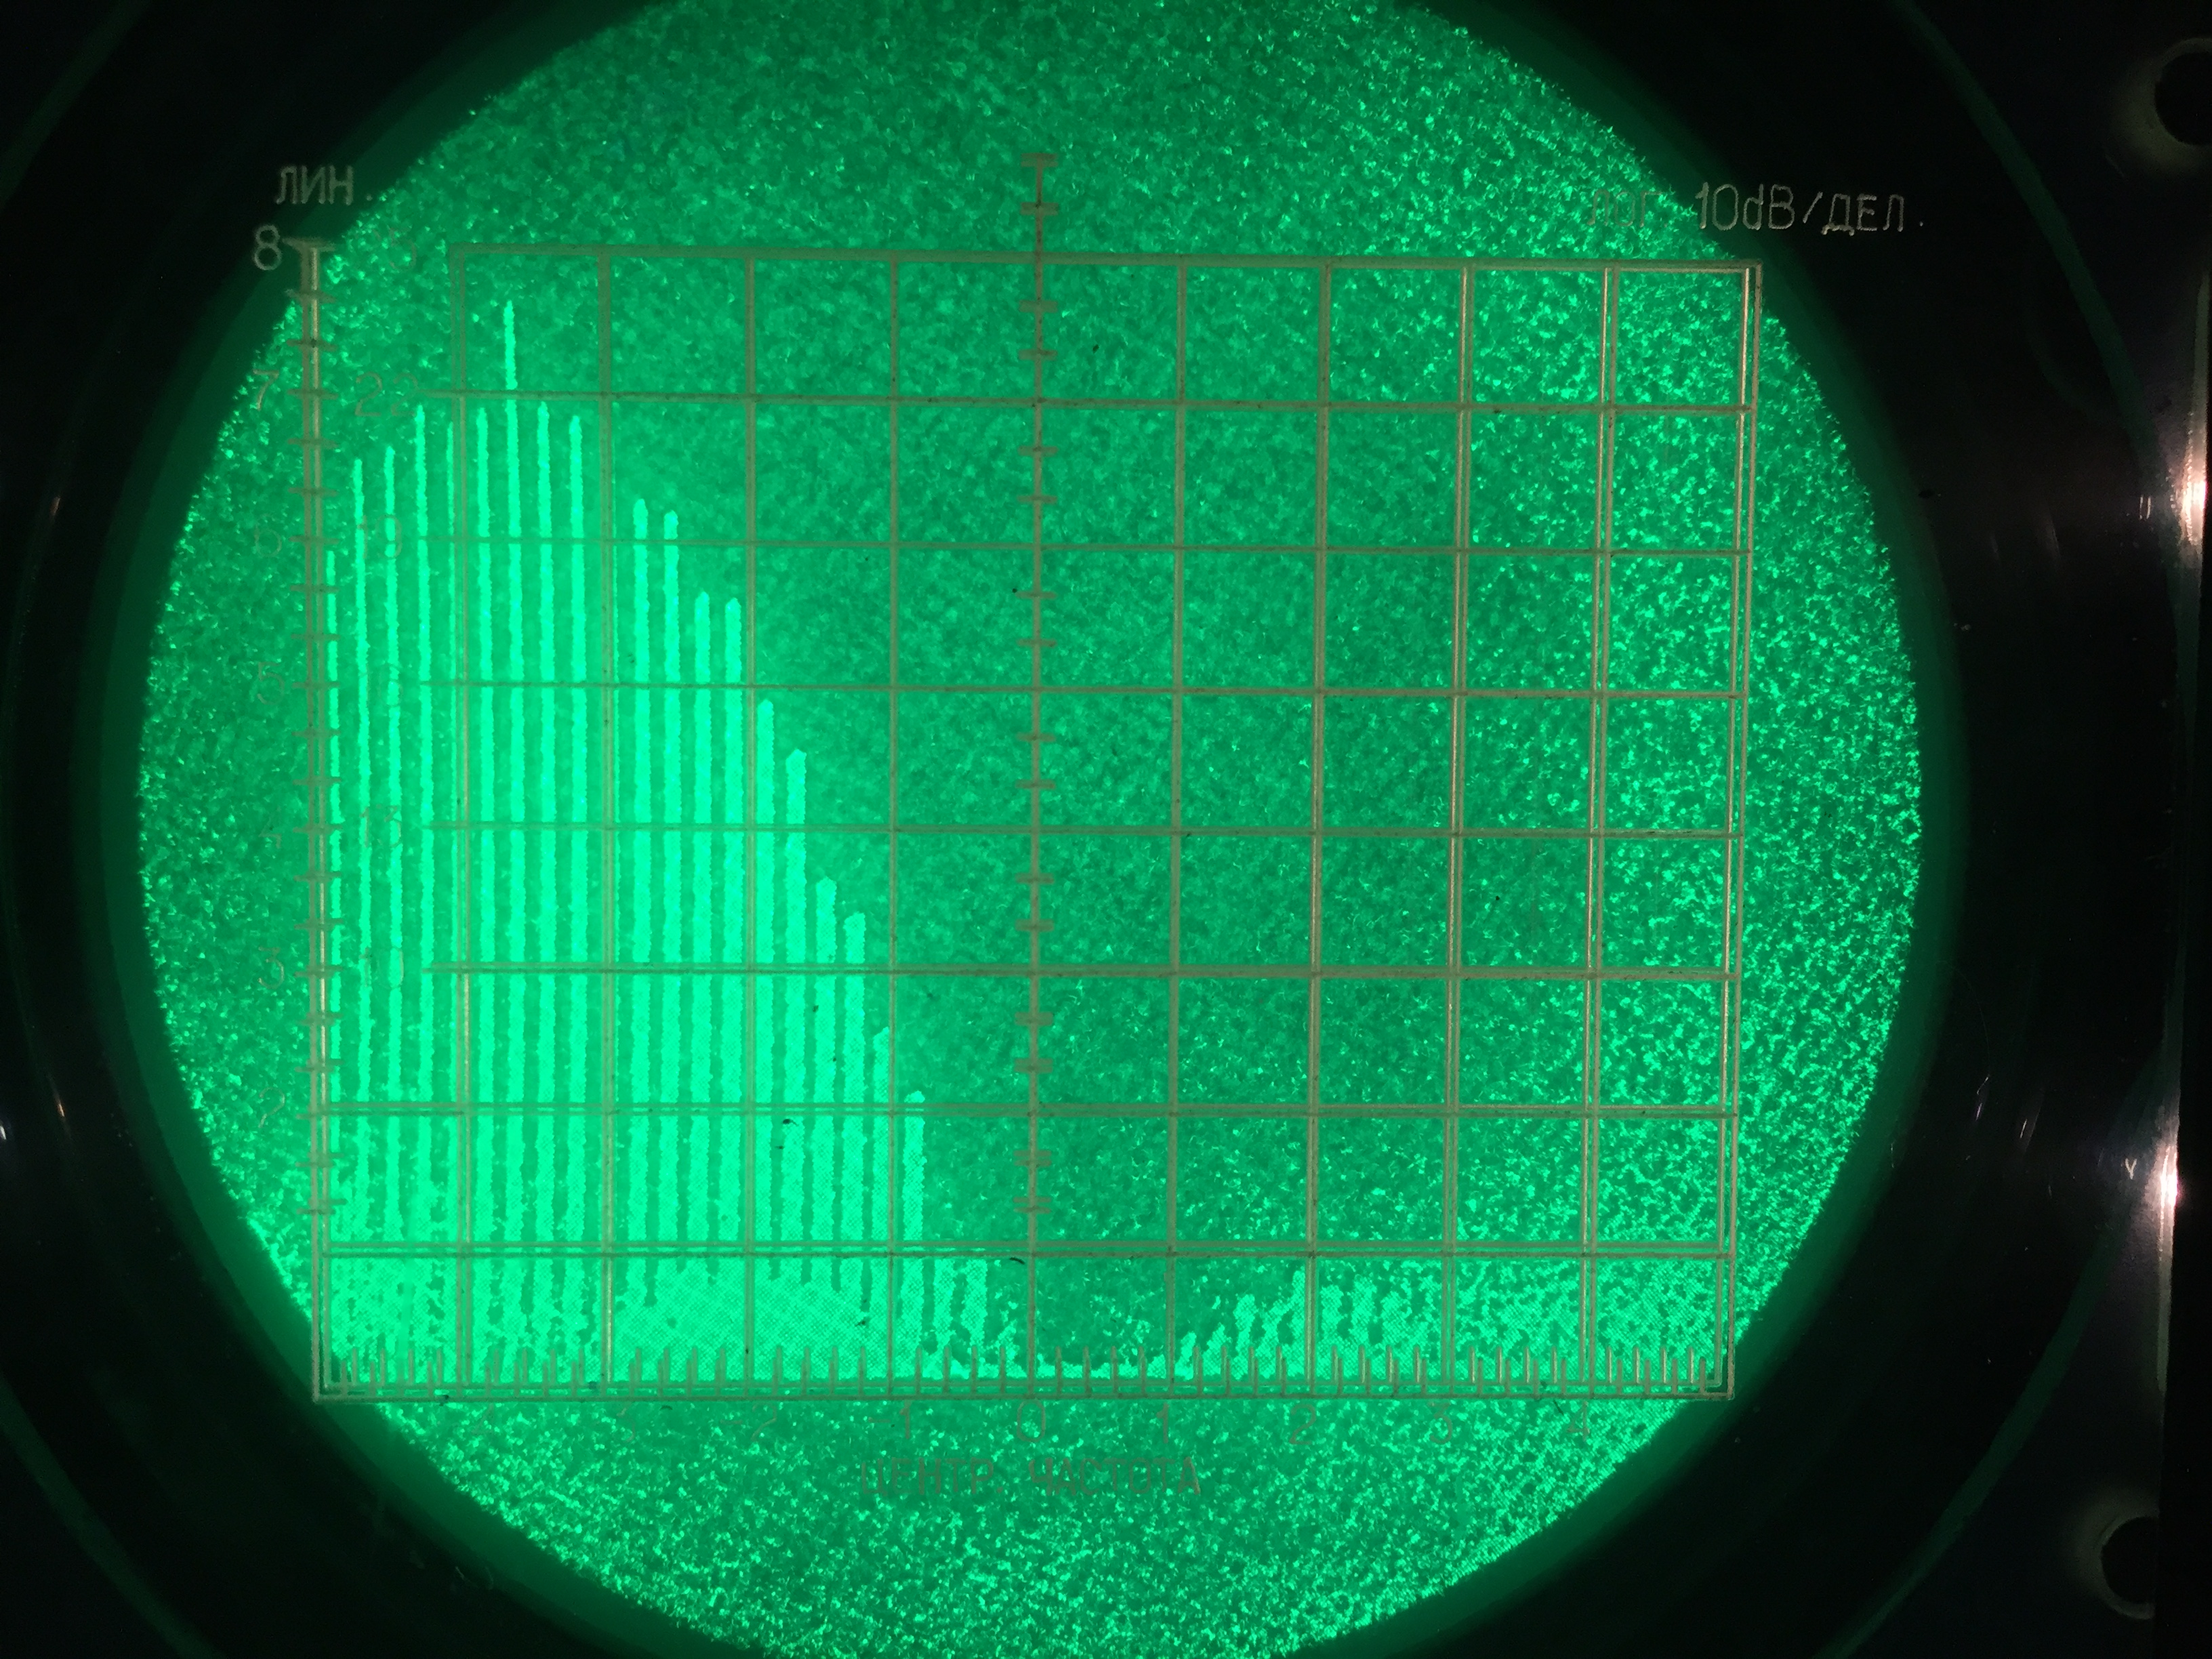
\includegraphics[width=0.9\linewidth]{IMG_0643} \\ а)$ \nu_{\text{0}} = 10 \text{кГц}$}
	\end{minipage}
	\begin{minipage}[h]{0.49\linewidth}
		\centering{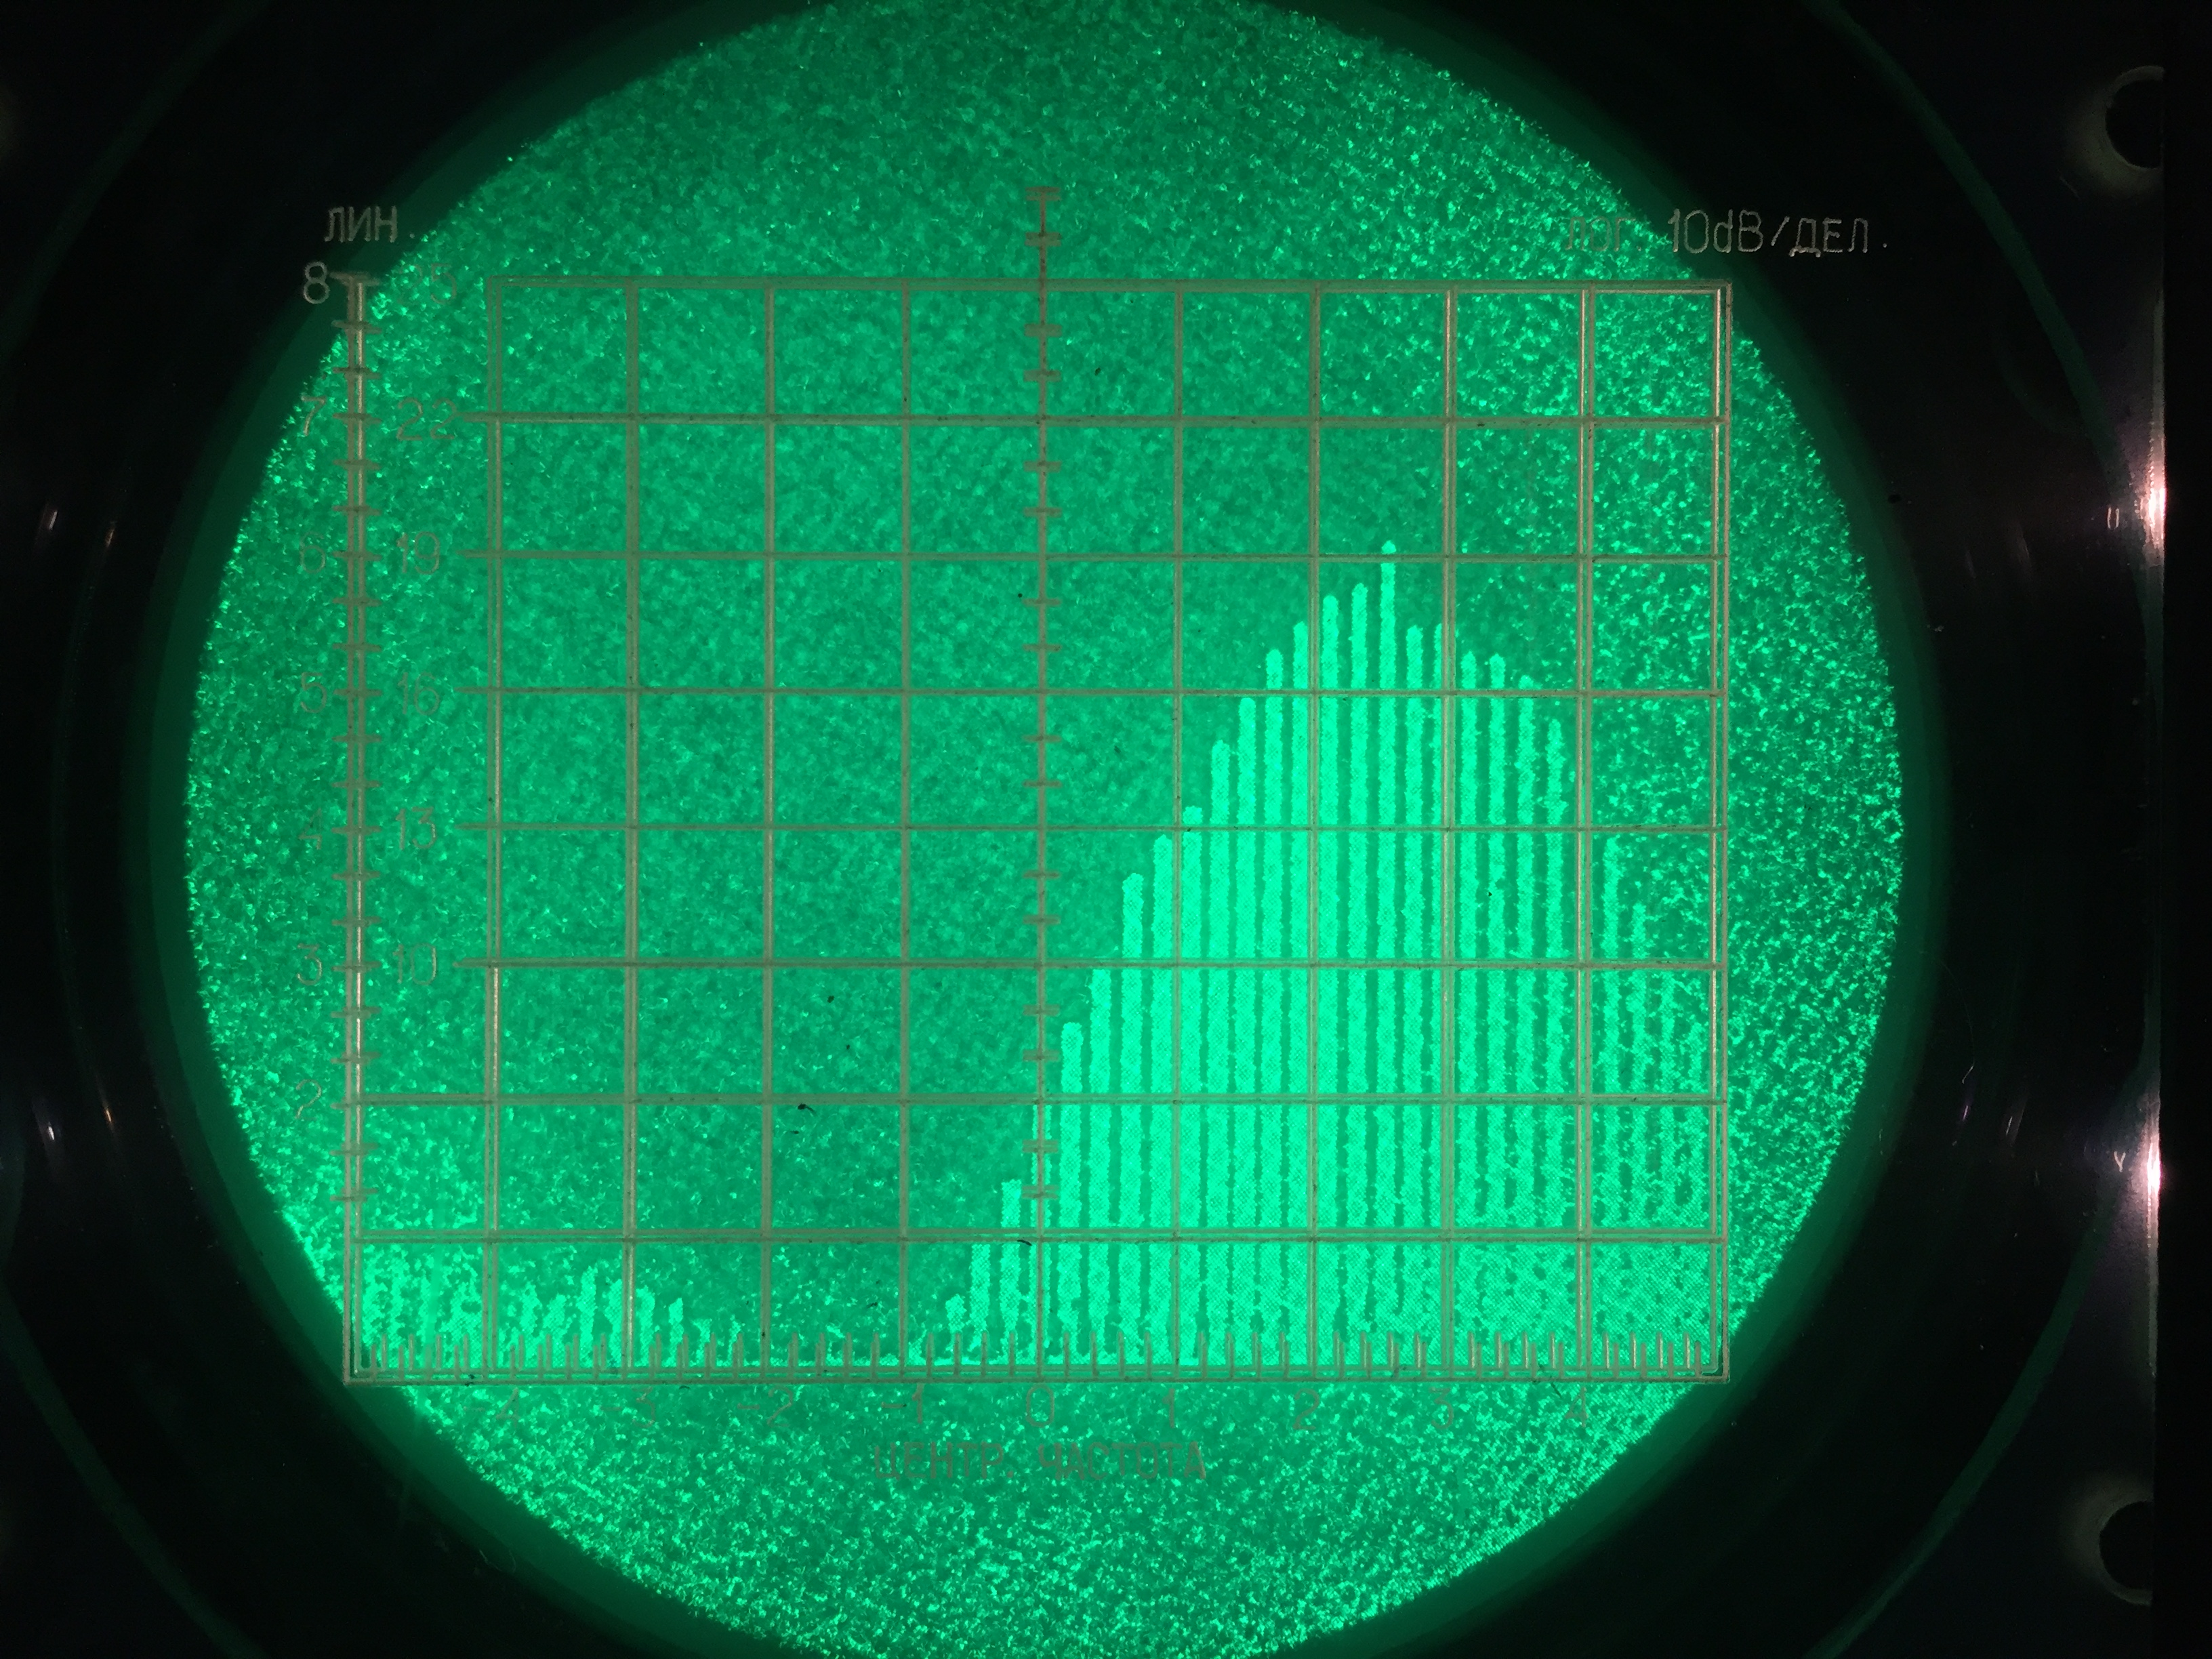
\includegraphics[width=0.9\linewidth]{IMG_0644} \\ б)$ \nu_{\text{0}} = 40 \text{кГц}$}
	\end{minipage}
	
	\caption{Зависимость спектра от частоты несущей $\nu_{0}$ при частоте $f_{\text{повт}} = 1\text{кГц}$ и длительности импульса $\tau = 50_{\text{мкс}}$.}
	\label{ris:image2}
\end{figure}



\begin{table}[H]
	\centering
	\caption{Зависимость расстояния между соседними спектральными компонентами от $f_\text{повт}$ при $\tau = 50 \text{мкс}$ }
	\label{my-label}
	\begin{tabular}{|c|c|c|c|c|c|c|c|c}
		\hline
		$f_\text{повт}, \text{кГц}$ & 1 & 2 & 3 & 4 & 5 & 6 & 7 & \multicolumn{1}{c|}{8} \\ \hline
		$\delta \nu, \text{кГц}$    & 1 & 2 & 3 & 4 & 5 & 6 & 7 & \multicolumn{1}{c|}{8} \\ \hline
		$\sigma \delta \nu, \text{кГц}$         & \multicolumn{8}{c|}{0,5}                           \\ \hline
	\end{tabular}
\end{table}

\begin{figure}[H]
\centering
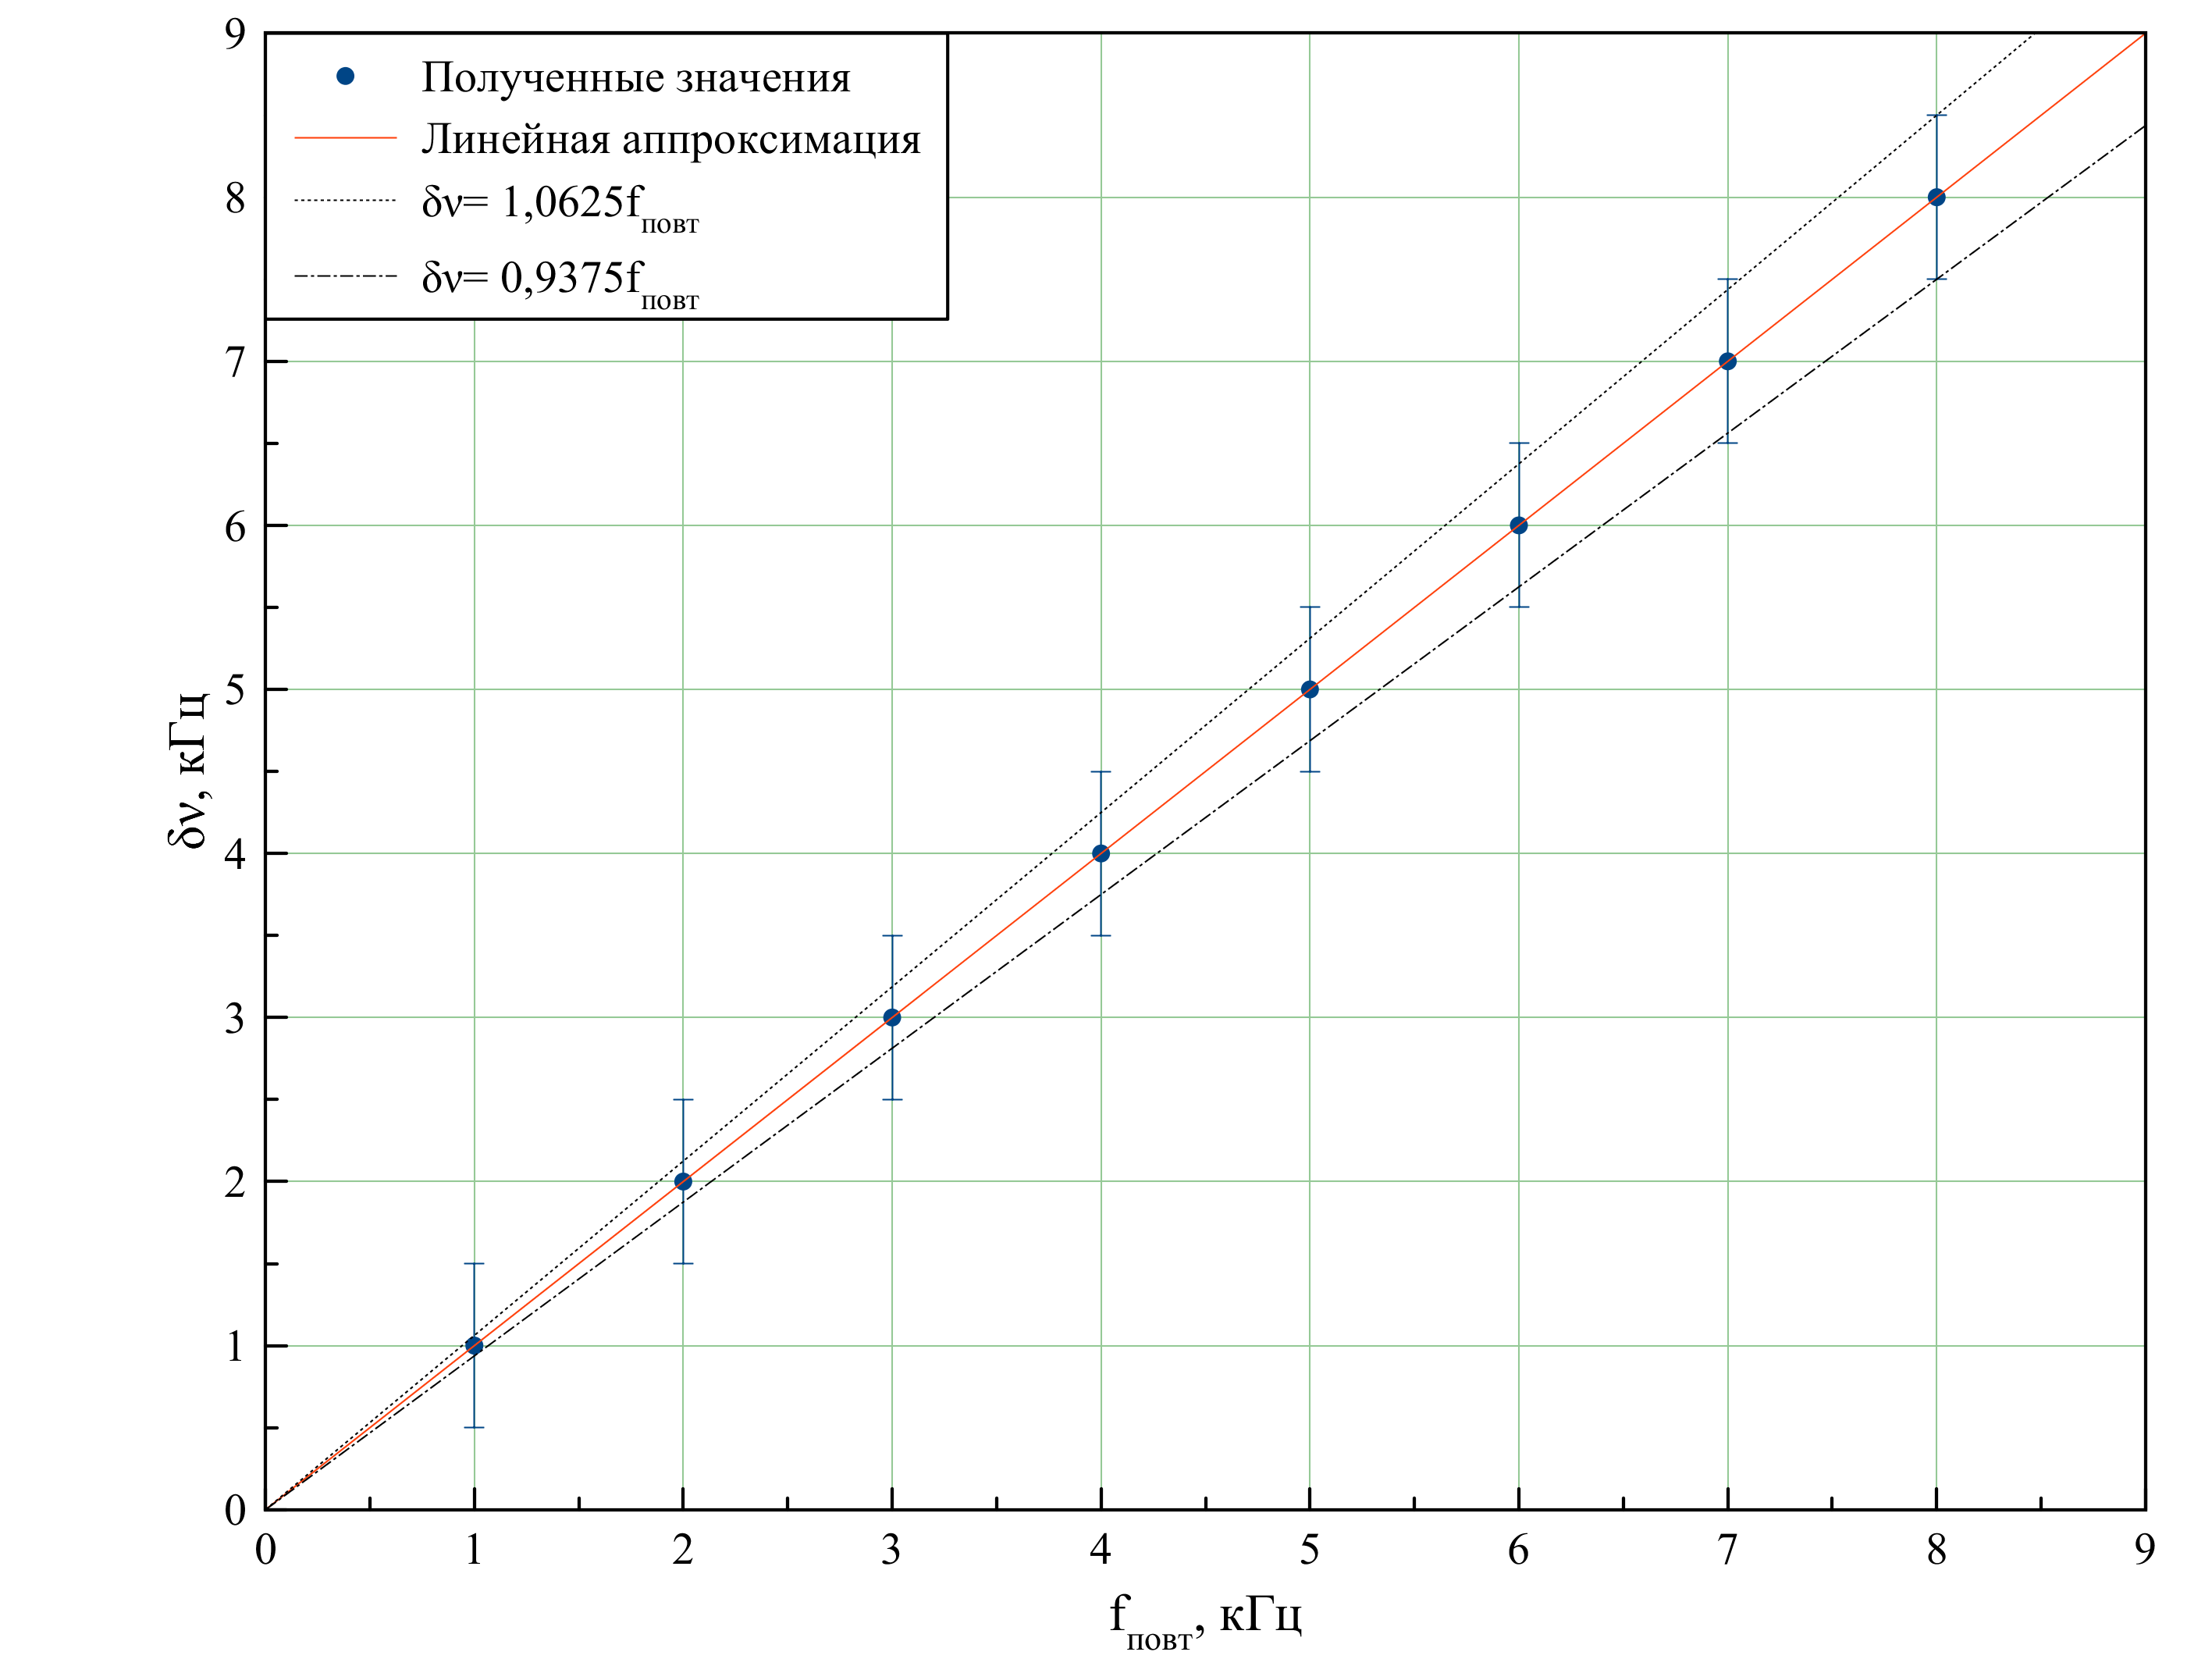
\includegraphics[width = \textwidth]{graphic}
\caption{График зависимости $\delta \nu (f_\text{повт})$}
\end{figure}

Коэффициент угла наклона прямой и его погрешность найдём из графика(проведём прямые с максимальным отклонением, учитывая погрешность $\sigma\delta\nu$ ): 
\begin{equation*}
\fbox{$
\Delta \nu \tau = 1,0000 \pm 0,0625(\varepsilon = 6 \%)$}
\end{equation*}

\begin{figure}[H]
	\centering
	
	\begin{minipage}[h]{0.49\linewidth}
		\centering{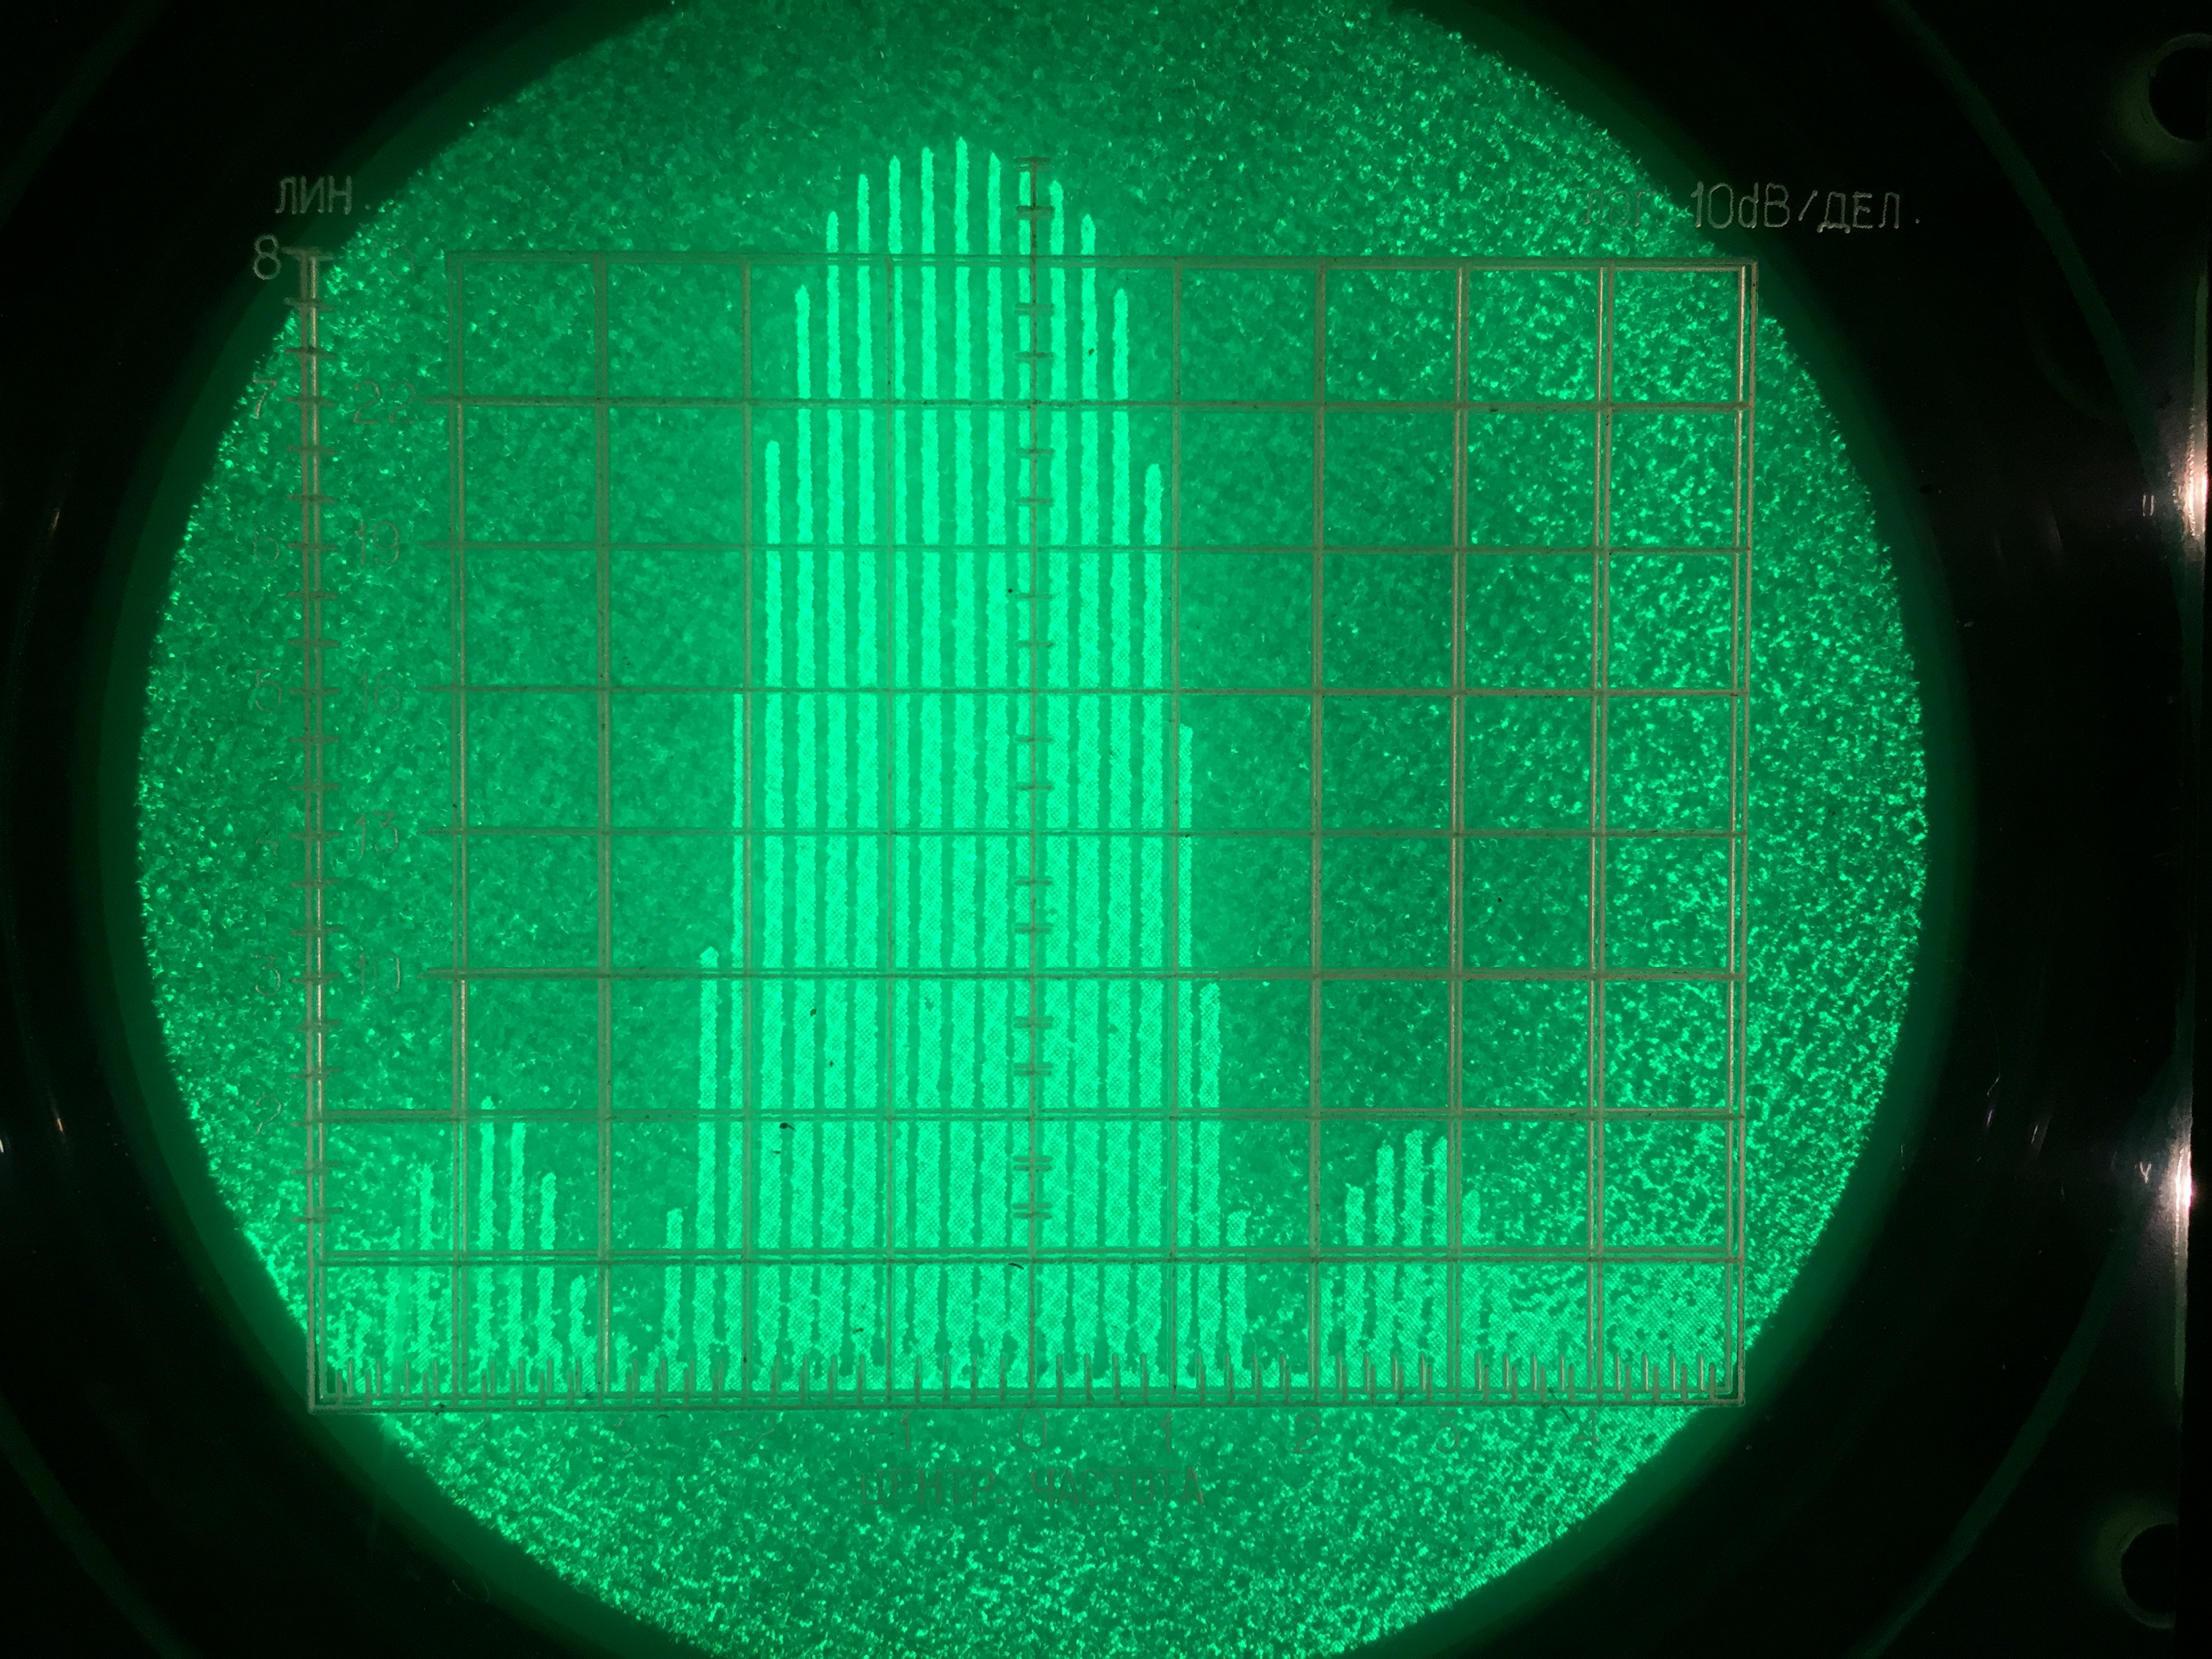
\includegraphics[width=0.9\linewidth]{IMG_0655} \\ а)$ f_{\text{повт}} = 1 \text{кГц}$}
	\end{minipage}
	\begin{minipage}[h]{0.49\linewidth}
		\centering{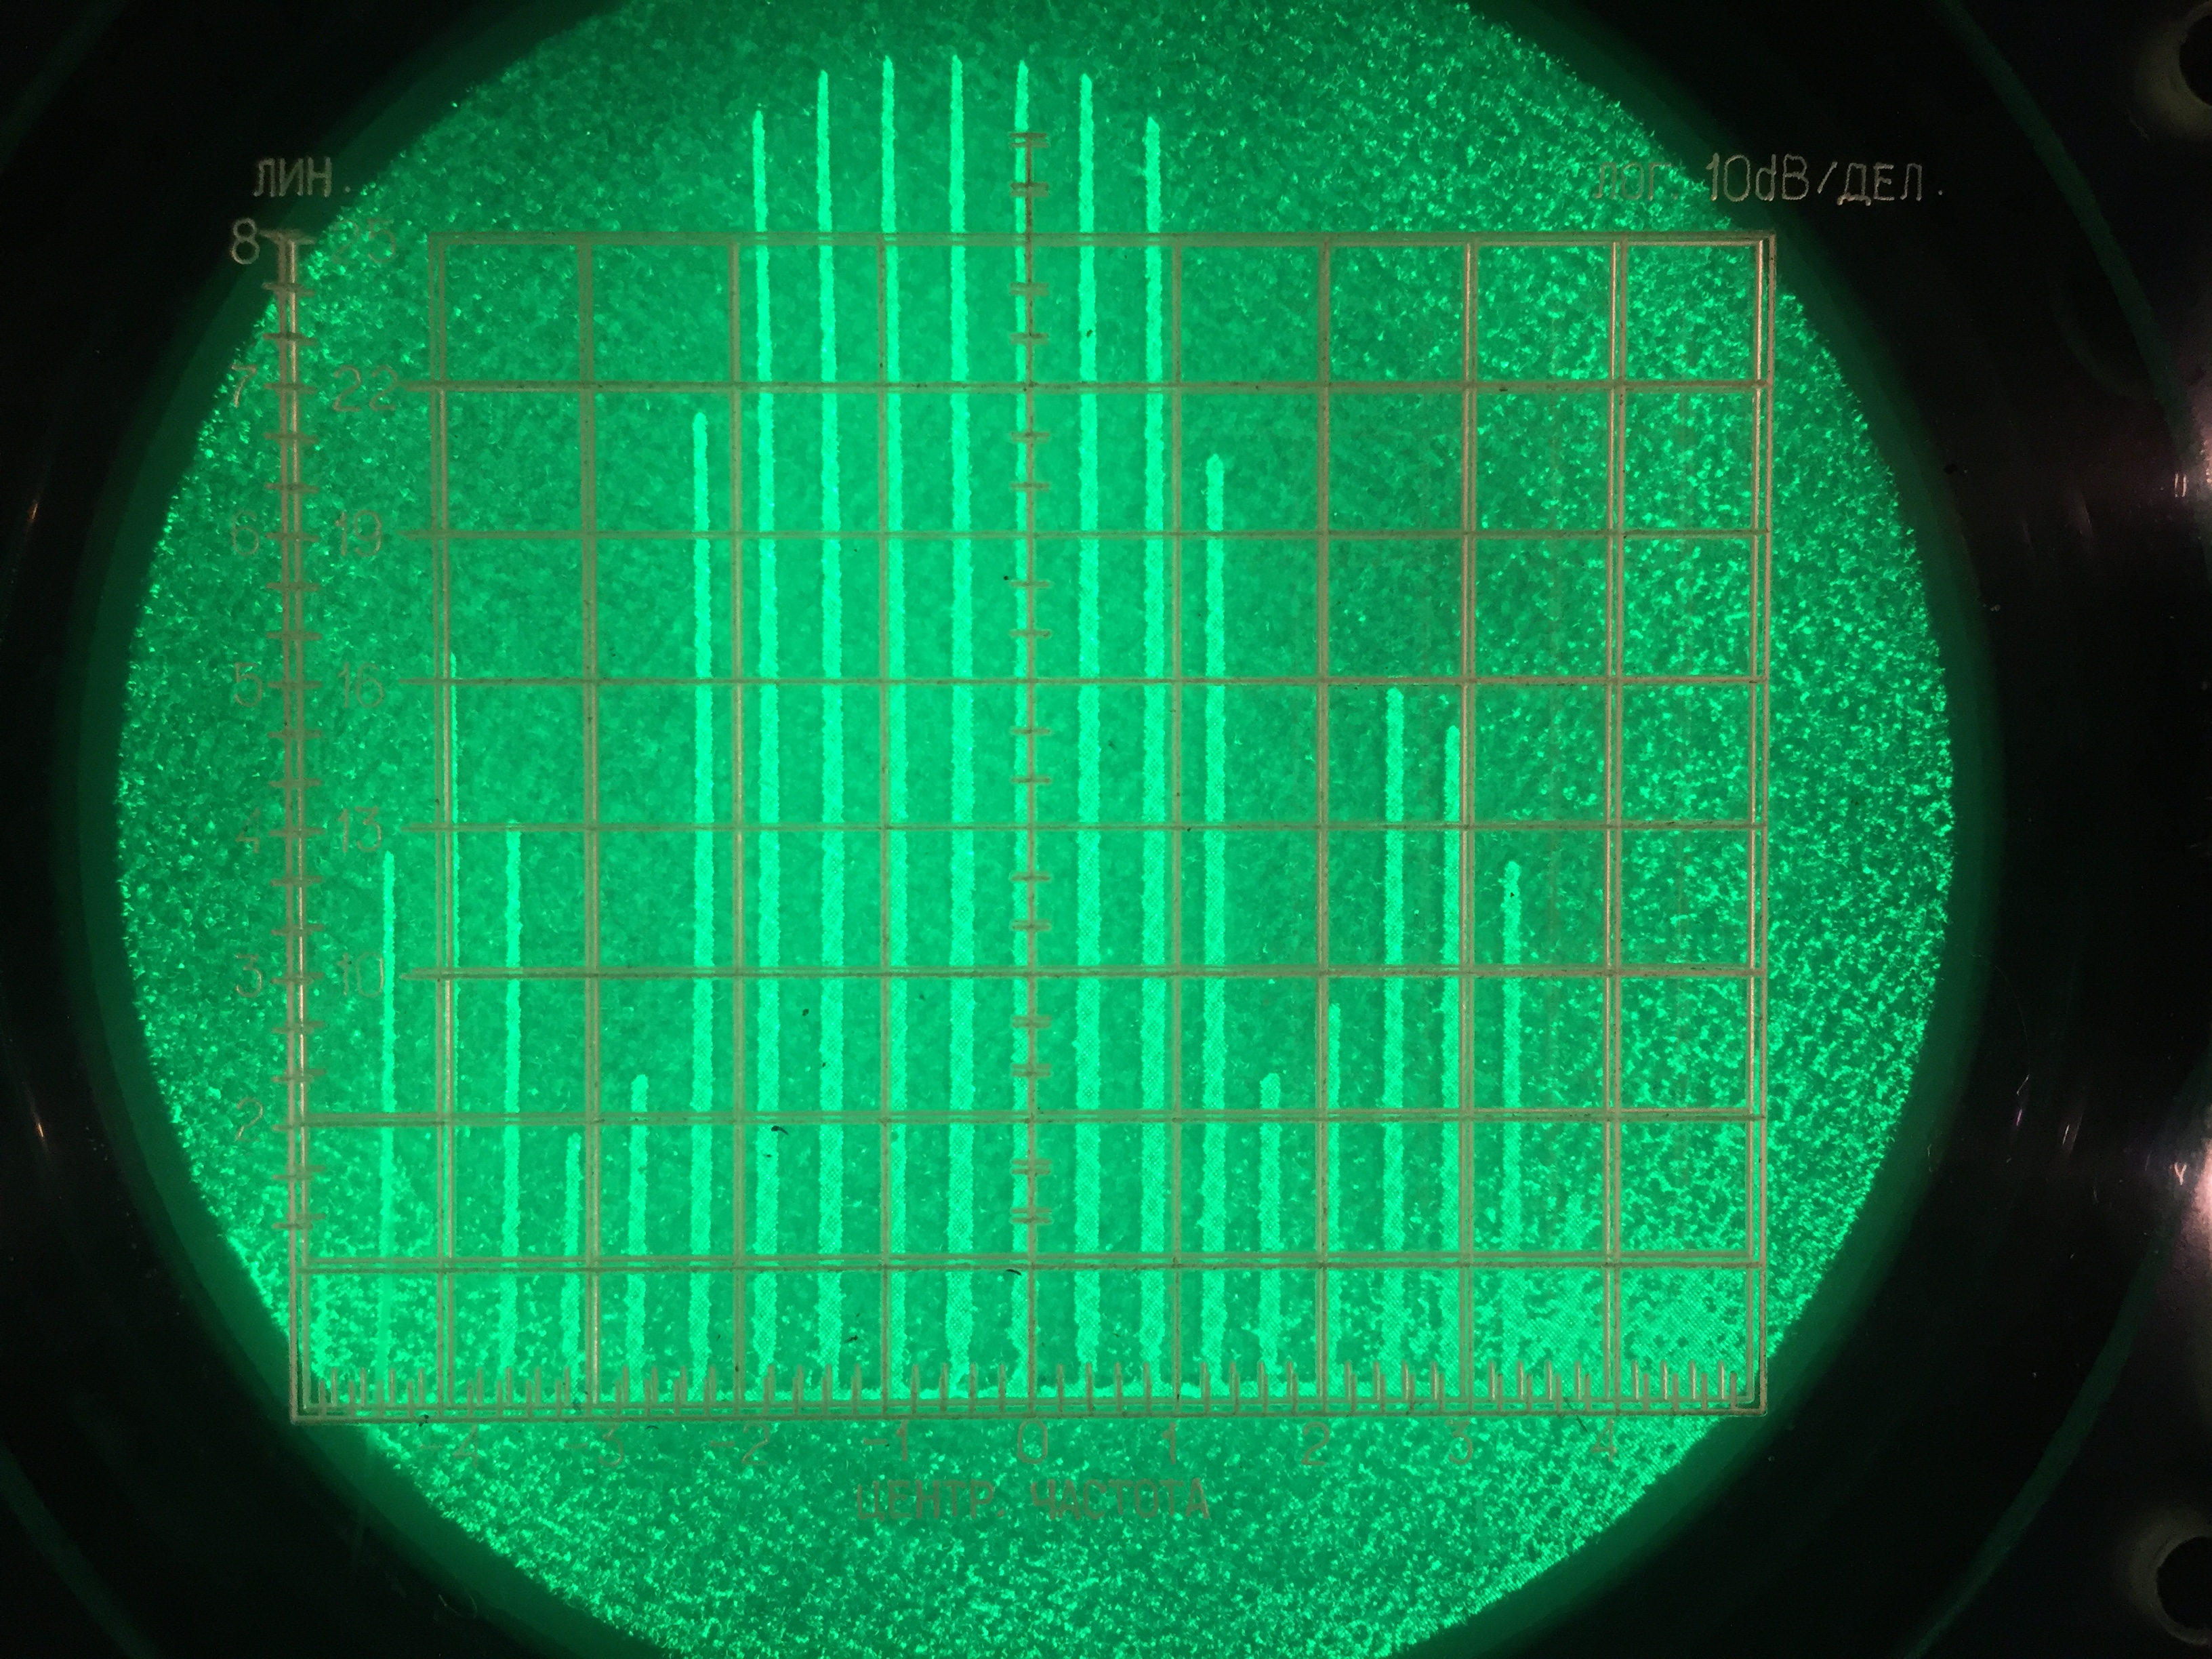
\includegraphics[width=0.9\linewidth]{IMG_0656} \\ б)$ f_{\text{повт}} = 2 \text{кГц}$}
	\end{minipage}
	
	\caption{Зависимость спектра от частоты повторения импульсов $f_{повт}$ при фиксированной длительности импульса  $\tau = 100\text{мкс}$.}
	\label{ris:image2}
\end{figure}

\subsection*{Исследование спектра гармонических сигналов, модулированных по амплитуде}

Рассмотрим гармонические колебания высокой частоты $\omega_0$, амплитуда которых медленно меняется по гармоническому закону с частотой $\Omega \ll \omega_0$.

\begin{equation}
\label{form:amf(t)_a_n}
	f(t) = A_0[1+m\cos(\Omega t)]\cos(\omega_0t)
\end{equation}

Коэффициент $m$ - {\it{глубина модуляции}} и по определению:
\begin{equation}
\label{form:m}
	m = \frac{A_{max}-A_{min}}{A_{max}+A_{min}}
\end{equation}

\subsubsection*{Выполнение}
В работе используются: \textit{анализатор спектра СК4-56; генератор прямоугольных импульсов Г5-54; осциллограф; генератор сигналов Г6-34}

\begin{figure}[H]
\centering
\includegraphics[width = 0.8\textwidth]{schemeC}
\caption{Схема для исследования спектра гармонических сигналов, модулированных по амплитуде}
\label{img:scheme C}
\end{figure}

Собираем схему согласно рис.\ref{img:scheme C}. Получаем на экране осциллографа гармонический сигнал, модулированный по амплитуде. Подключаем анализатор спектра СК4-56 и после настройки наблюдаем спектр сигнала.

Чтобы измерить глубину модуляции, измерим $A_{max}$, $A_{min}$ и подставим в формулу \ref{form:m}. Построим график отношения $a_\text{бок}/a_\text{осн}$ в зависимости от $m$.

Рассчитаем теоретический коэффициент наклона, воспользовавшись формулой:
\begin{equation}
\label{form:a/a(m)}
	f(t)=A_0\cos(\omega_0t)+	\frac{A_0m}{2}\cos(\omega_0+\Omega t)+\frac{A_0m}{2}\cos(\omega_0-\Omega t). 
\end{equation}

$$a_\text{осн} = A_0, \; a_\text{бок}= \frac{A_0m}{2} \Rightarrow k_\text{теор} =0.5$$
	
\begin{table}[H]
\centering
\caption{Зависимость отношения амплитуды боковой линии спектра к амплитуде основной линии $a_\text{бок}/a_\text{осн}$ от глубины модуляции $m$.}
\begin{tabular}{|c|c|c|c|c|c|c|c|}
\hline
$2A_{min}, \text{дел}$ & $2A_{max}, \text{дел}$ & $m$  & $a_\text{бок}, \text{дел}$ & $a_\text{осн}, \text{дел}$ & $a_\text{бок}/a_\text{осн}$ & $\sigma_{a_\text{бок}/a_\text{осн}}$ & $\sigma_{m}$ \\ \hline
7                & 9                & 0,125 & 0                      & 30                   &0                         & 0     & 0,01                      \\ \hline
6                & 11                & 0,29 & 4                      & 30                      & 0,13                        & 0,02                         &0,03     \\ \hline
4                & 13                & 0,53 & 7		                      & 30                      & 0,23                        & 0,02                          &0,09     \\ \hline
0                & 16                & 1 & 13                      & 29                      & 0,45                        & 0,02                           &0,03    \\ \hline
\end{tabular}
\end{table}

\begin{figure}[H]
\centering
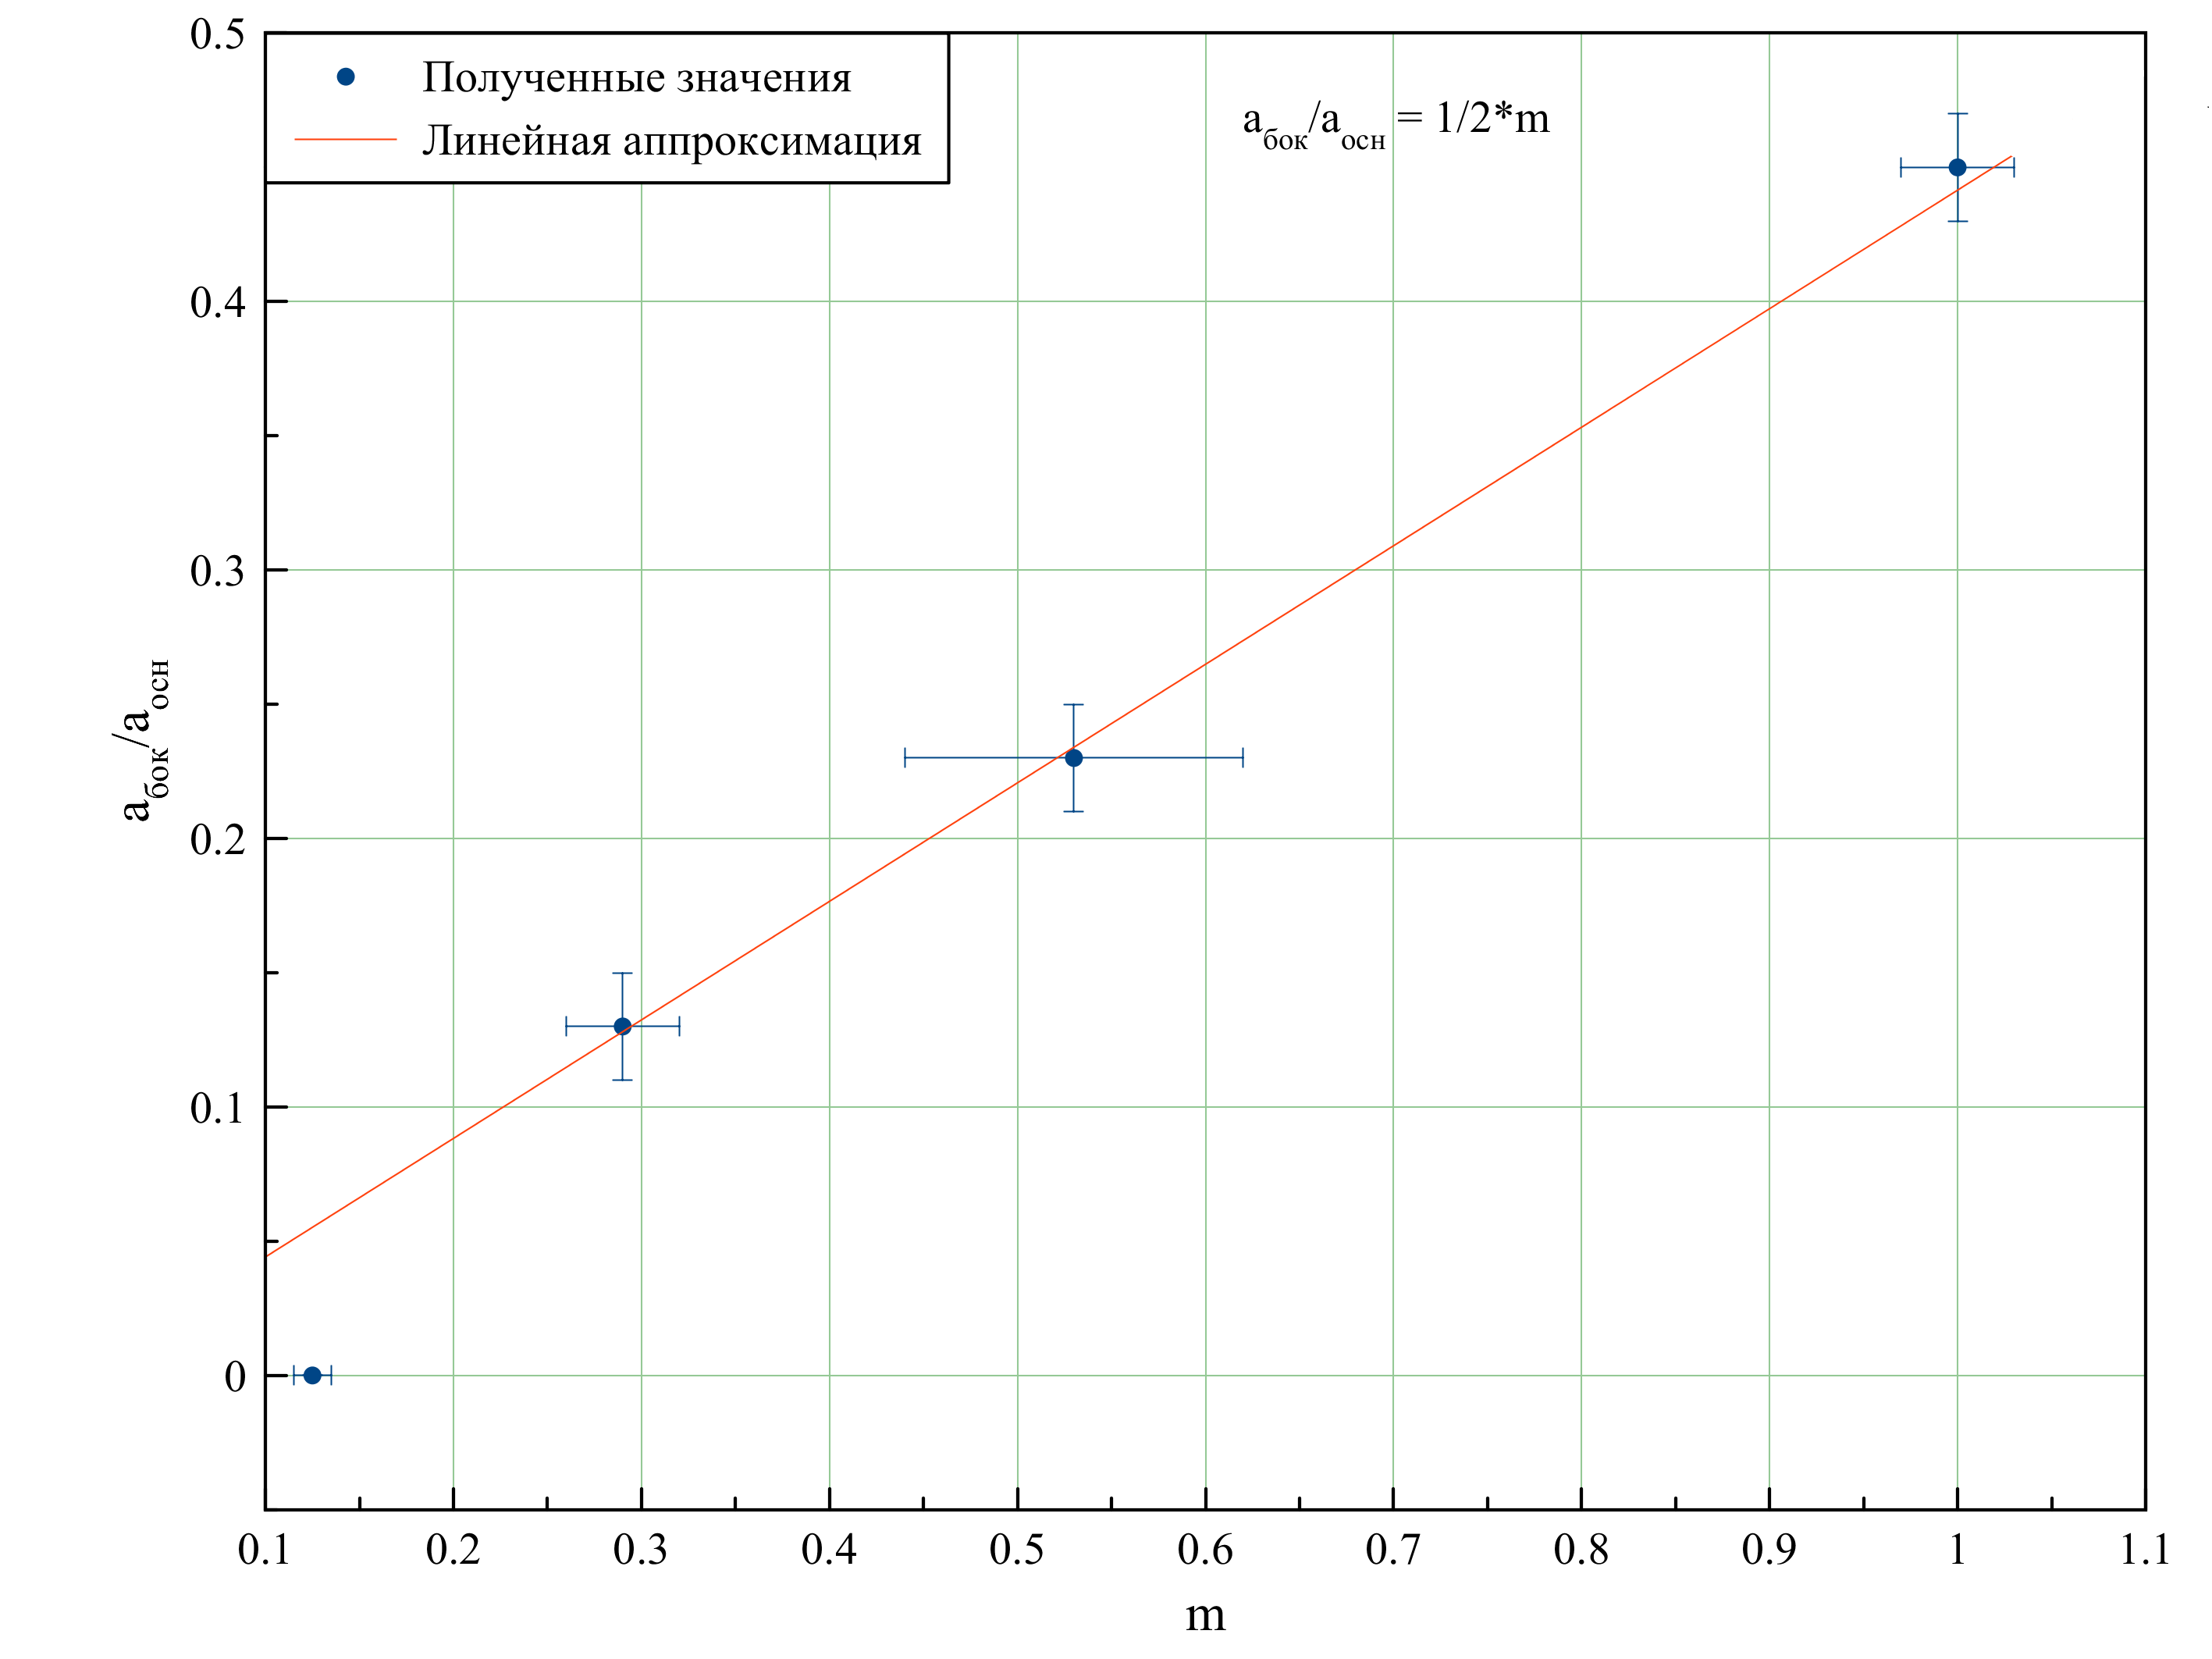
\includegraphics[width = \textwidth]{graphic2}
\caption{График зависимости $\dfrac{a_\text{бок}}{a_\text{осн}}(m)$}
\end{figure}

Коэффициент угла наклона прямой и его погрешность посчитаем методом наименьших квадратов: $k = \dfrac{\langle \frac{a_\text{бок} m}{a_\text{осн}}  \rangle}{\langle m^2 \rangle}$, $\sigma_k = \dfrac{1}{\sqrt{n}} \sqrt{\dfrac{\langle \left( \frac{a_\text{бок}}{a_\text{осн}}\right)^2 \rangle}{\langle m^2 \rangle} - k^2}$, тогда 
\begin{equation}
\fbox{$\dfrac{a_\text{бок}}{a_\text{осн} m} = 0.44 \pm 0.02(\varepsilon \simeq 5\%)$}
\end{equation}

\begin{figure}[H]
	\centering
		\begin{minipage}[h]{0.49\linewidth}
		\centering{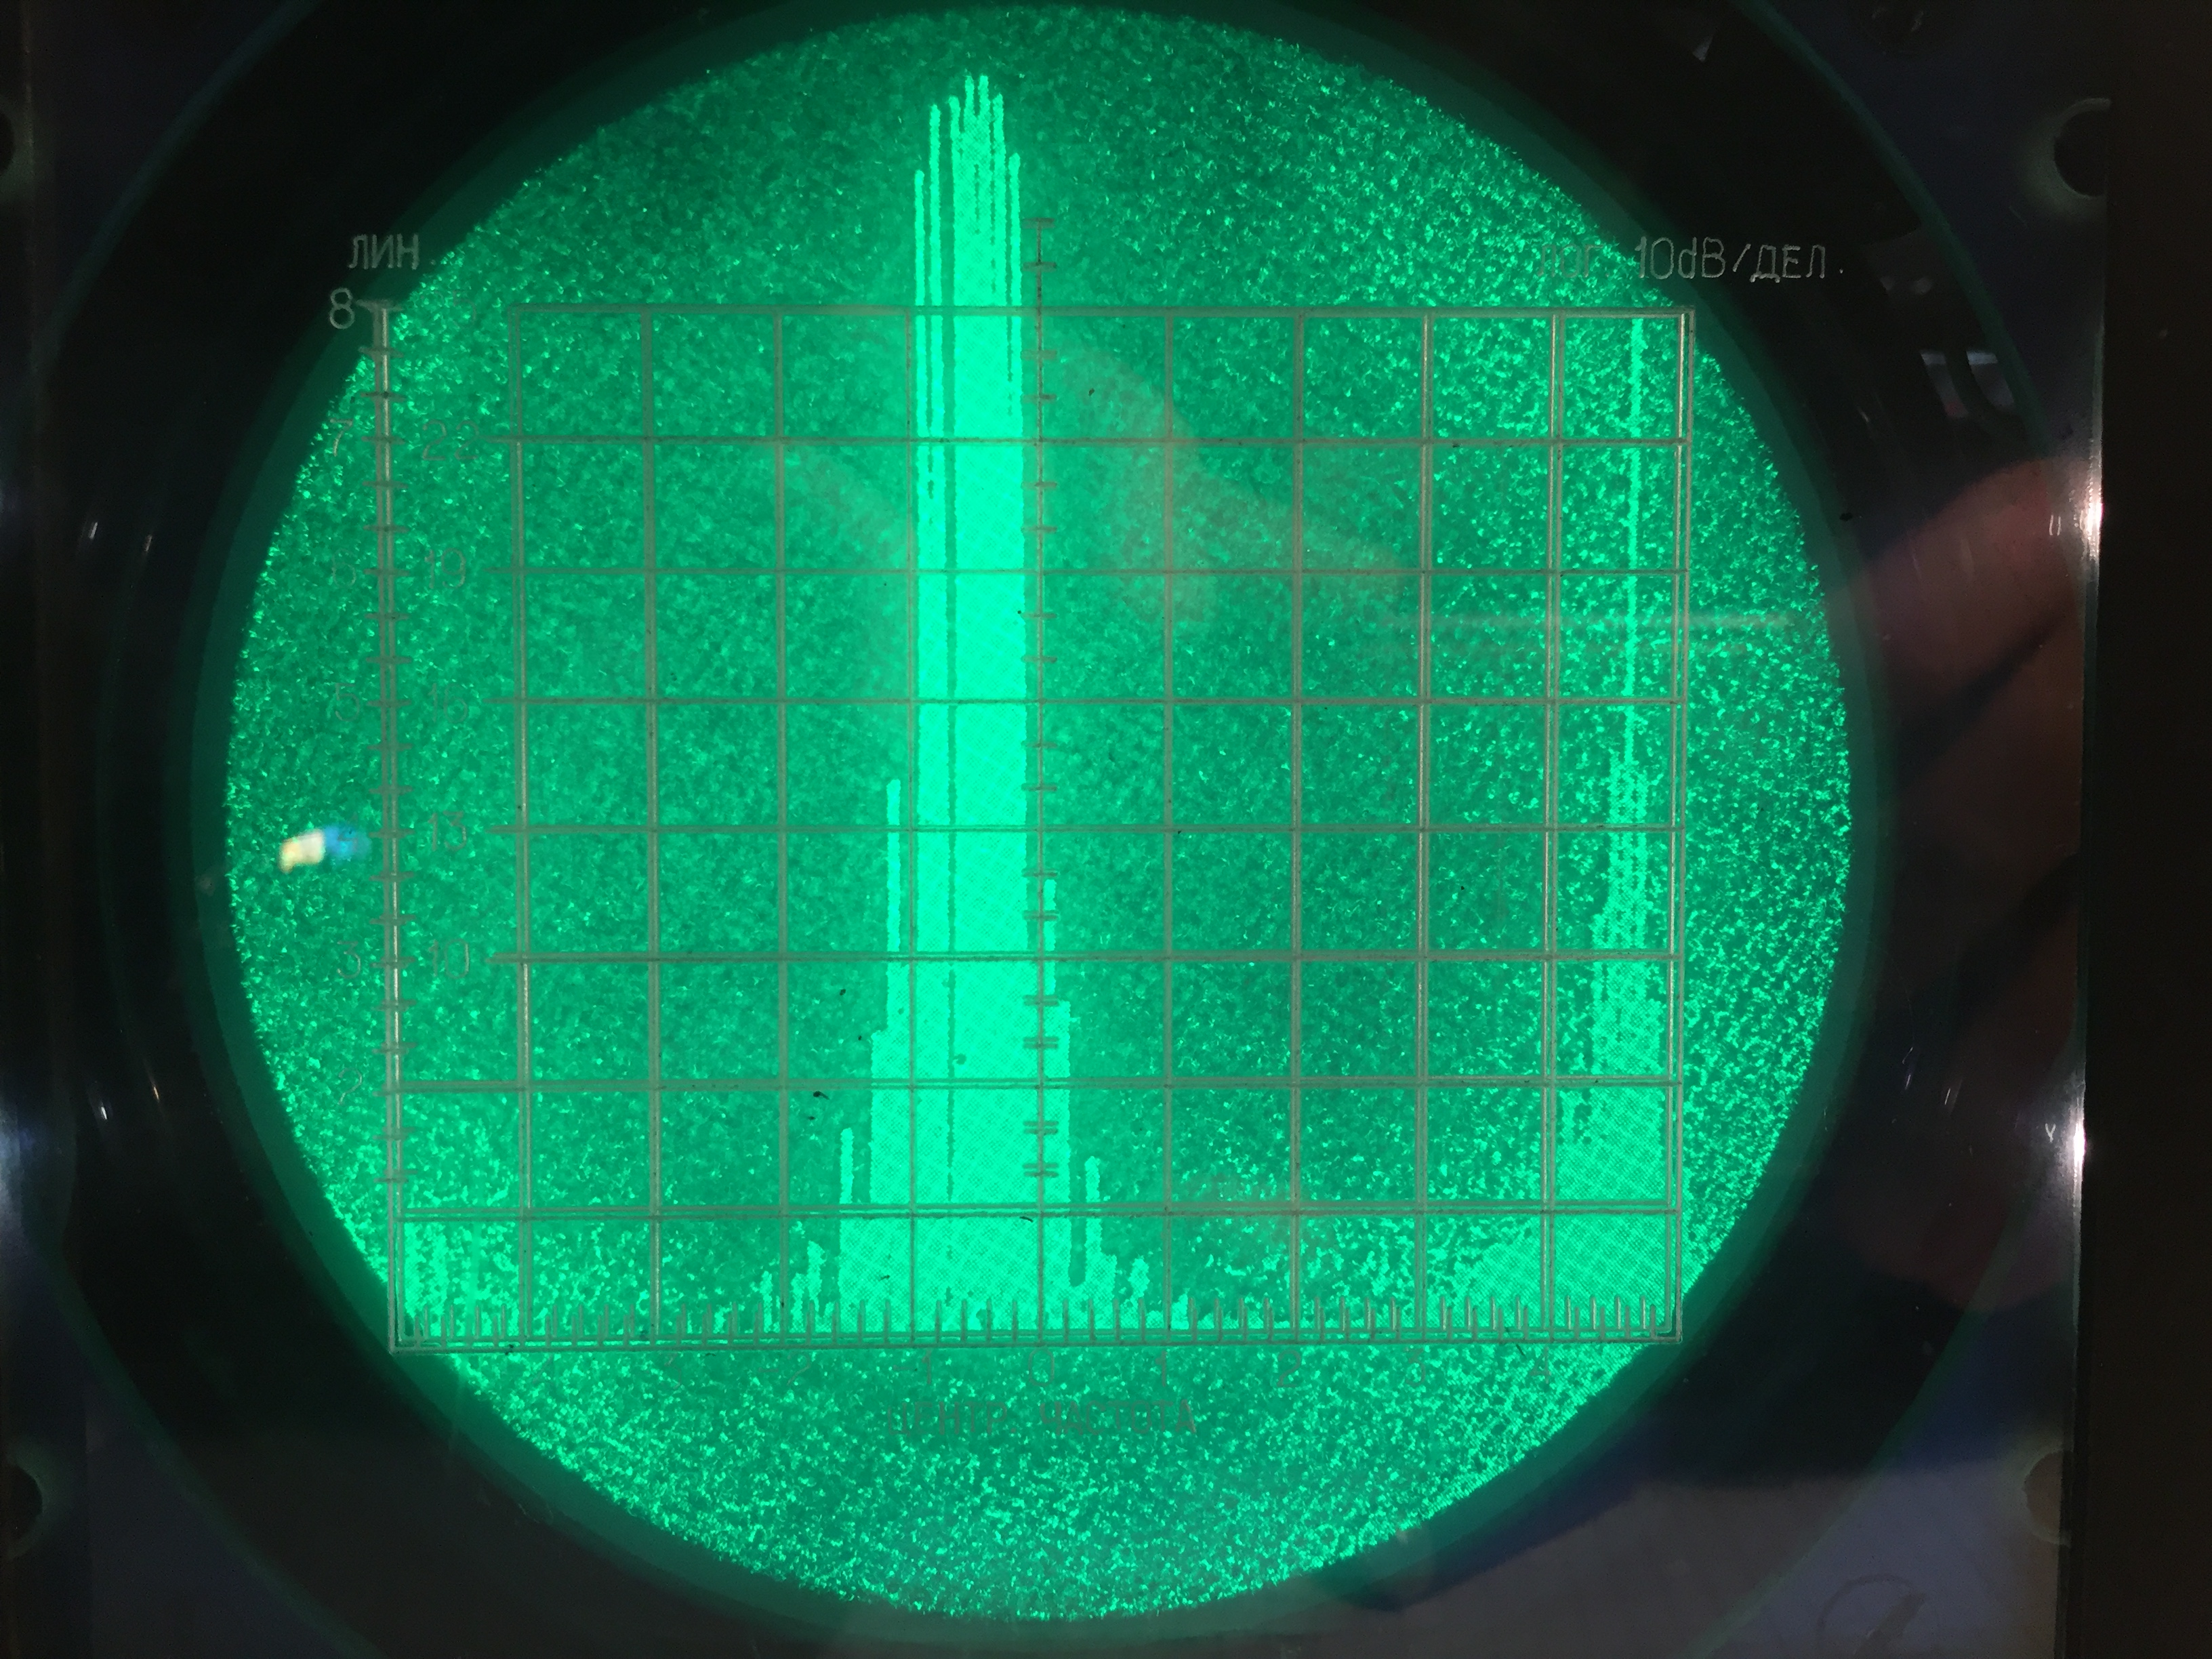
\includegraphics[width=0.9\linewidth]{IMG_0700}} \\[0,9cm] 
		
		\centering{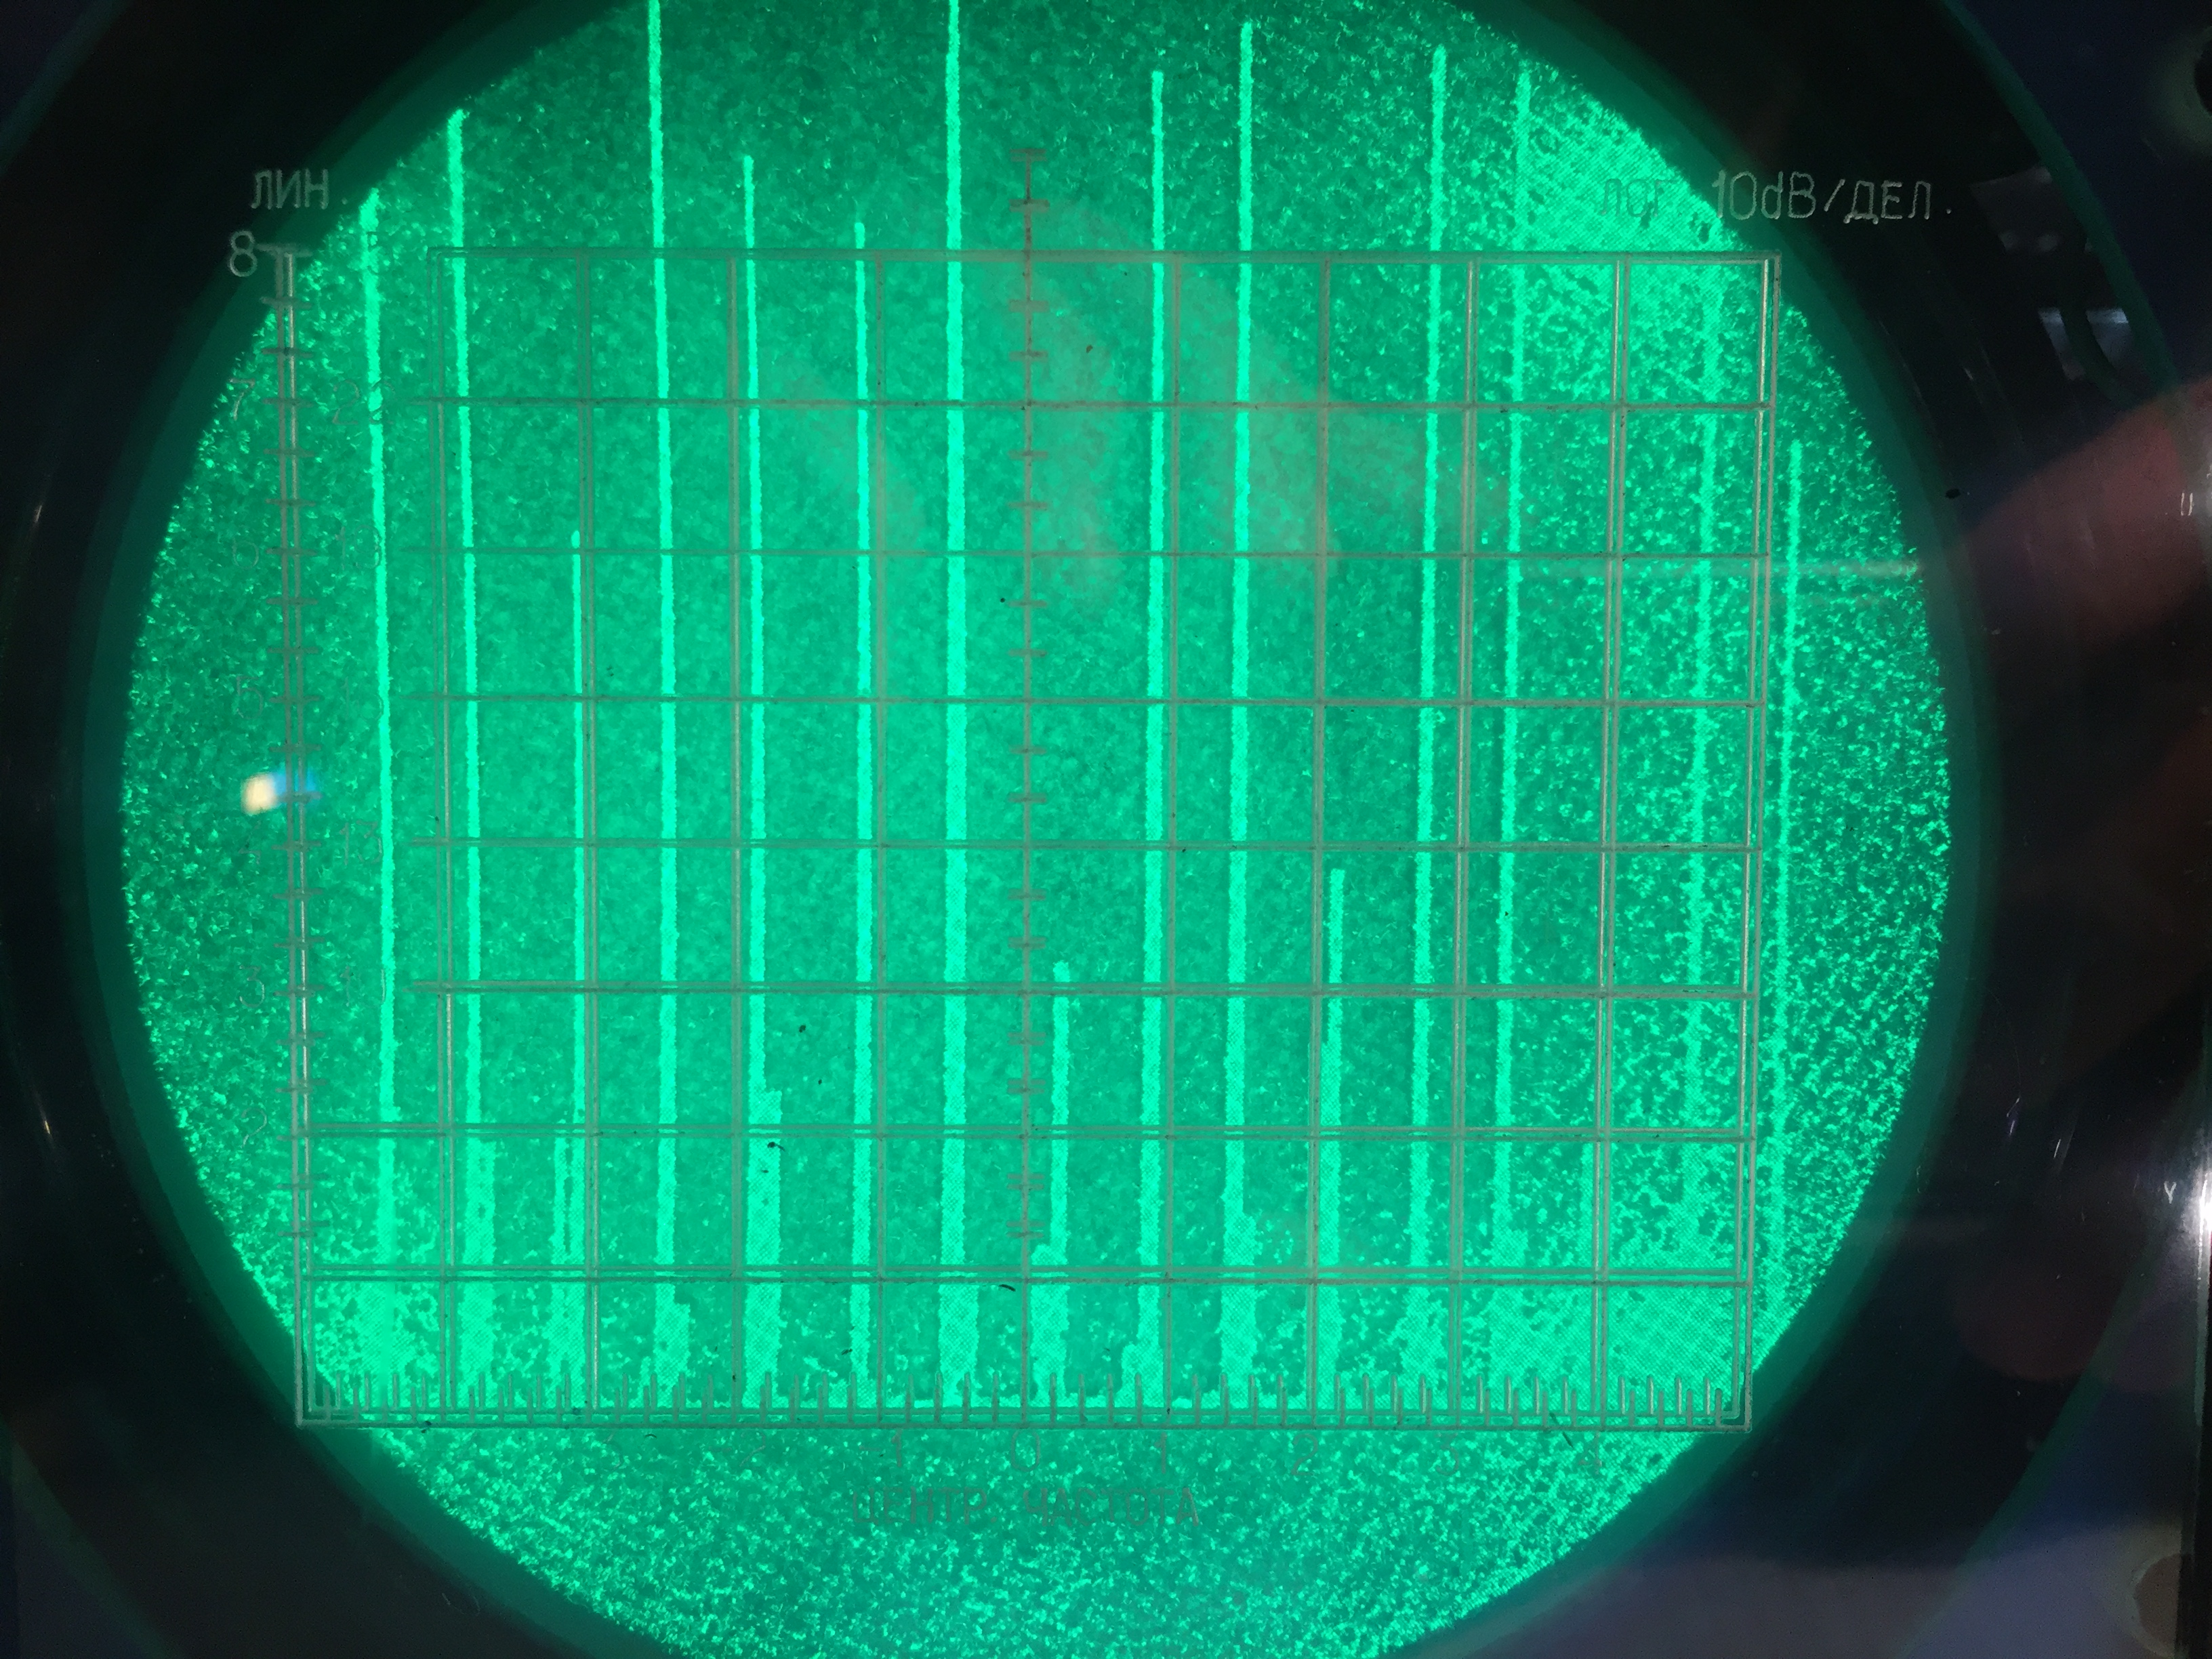
\includegraphics[width=0.9\linewidth]{IMG_0704}} \\ 
	\end{minipage}
	\begin{minipage}[h]{0.49\linewidth}
		\centering{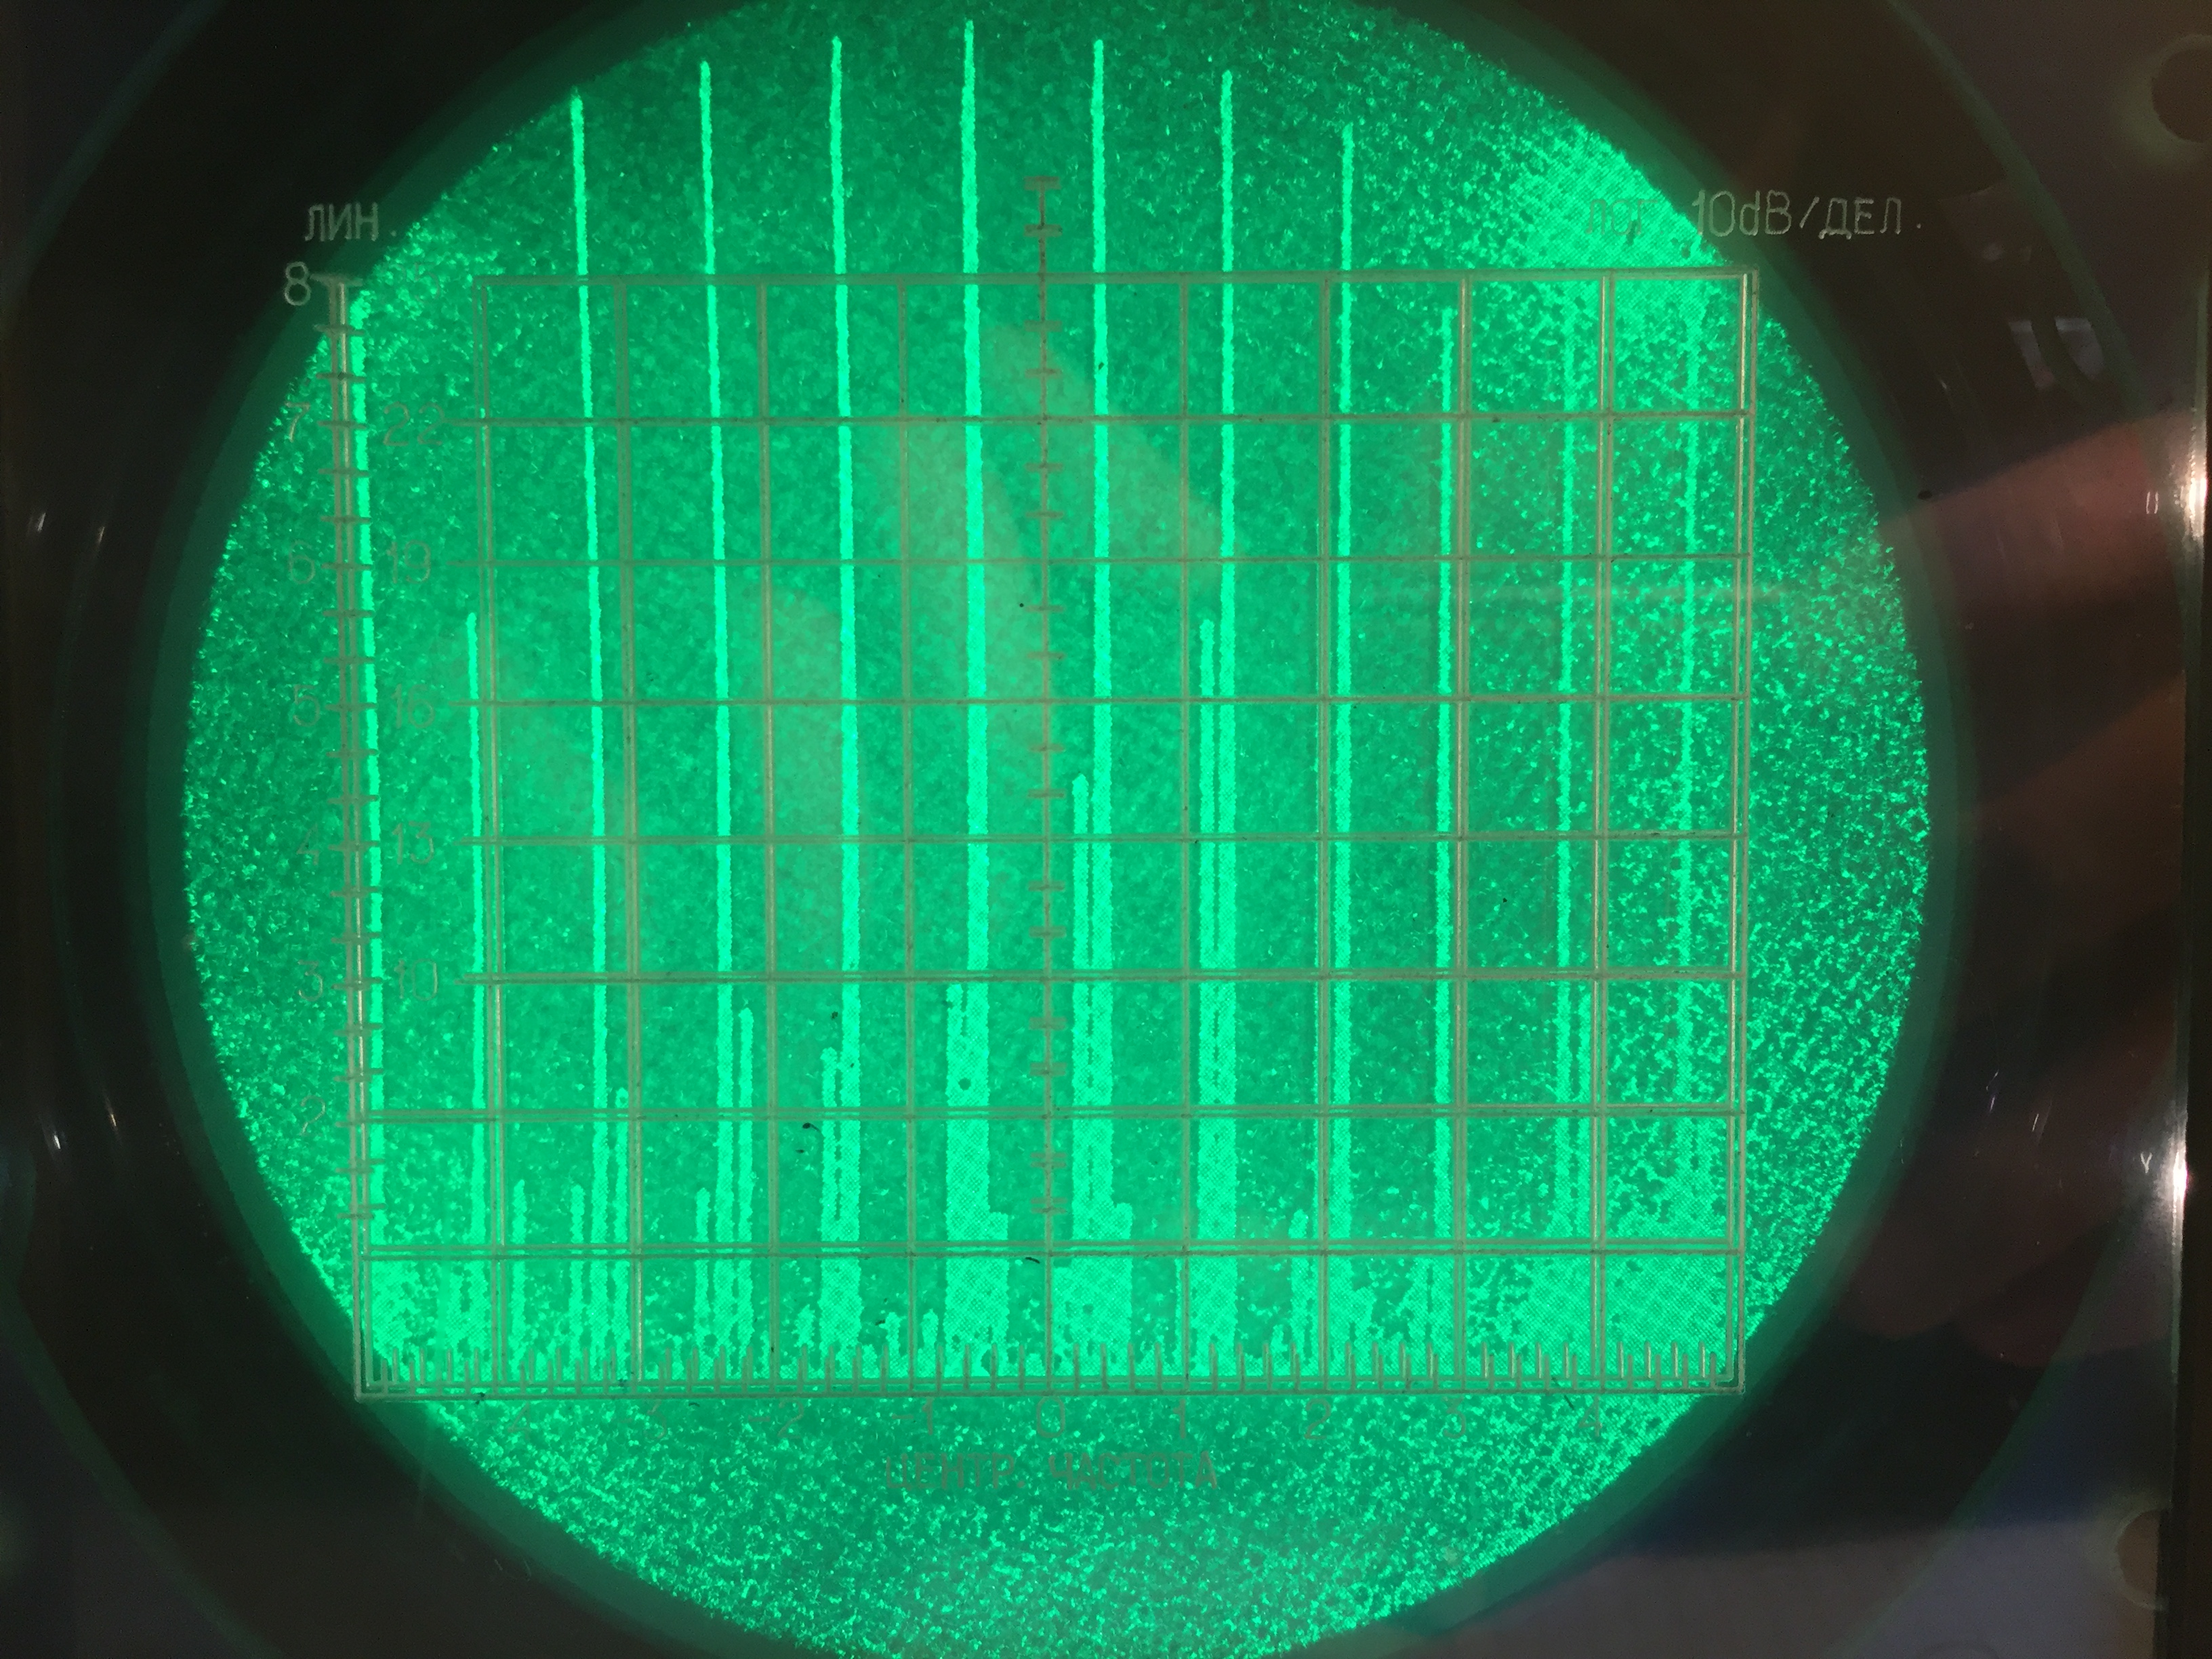
\includegraphics[width=0.9\linewidth]{IMG_0702}} \\[0,9cm]
		\centering{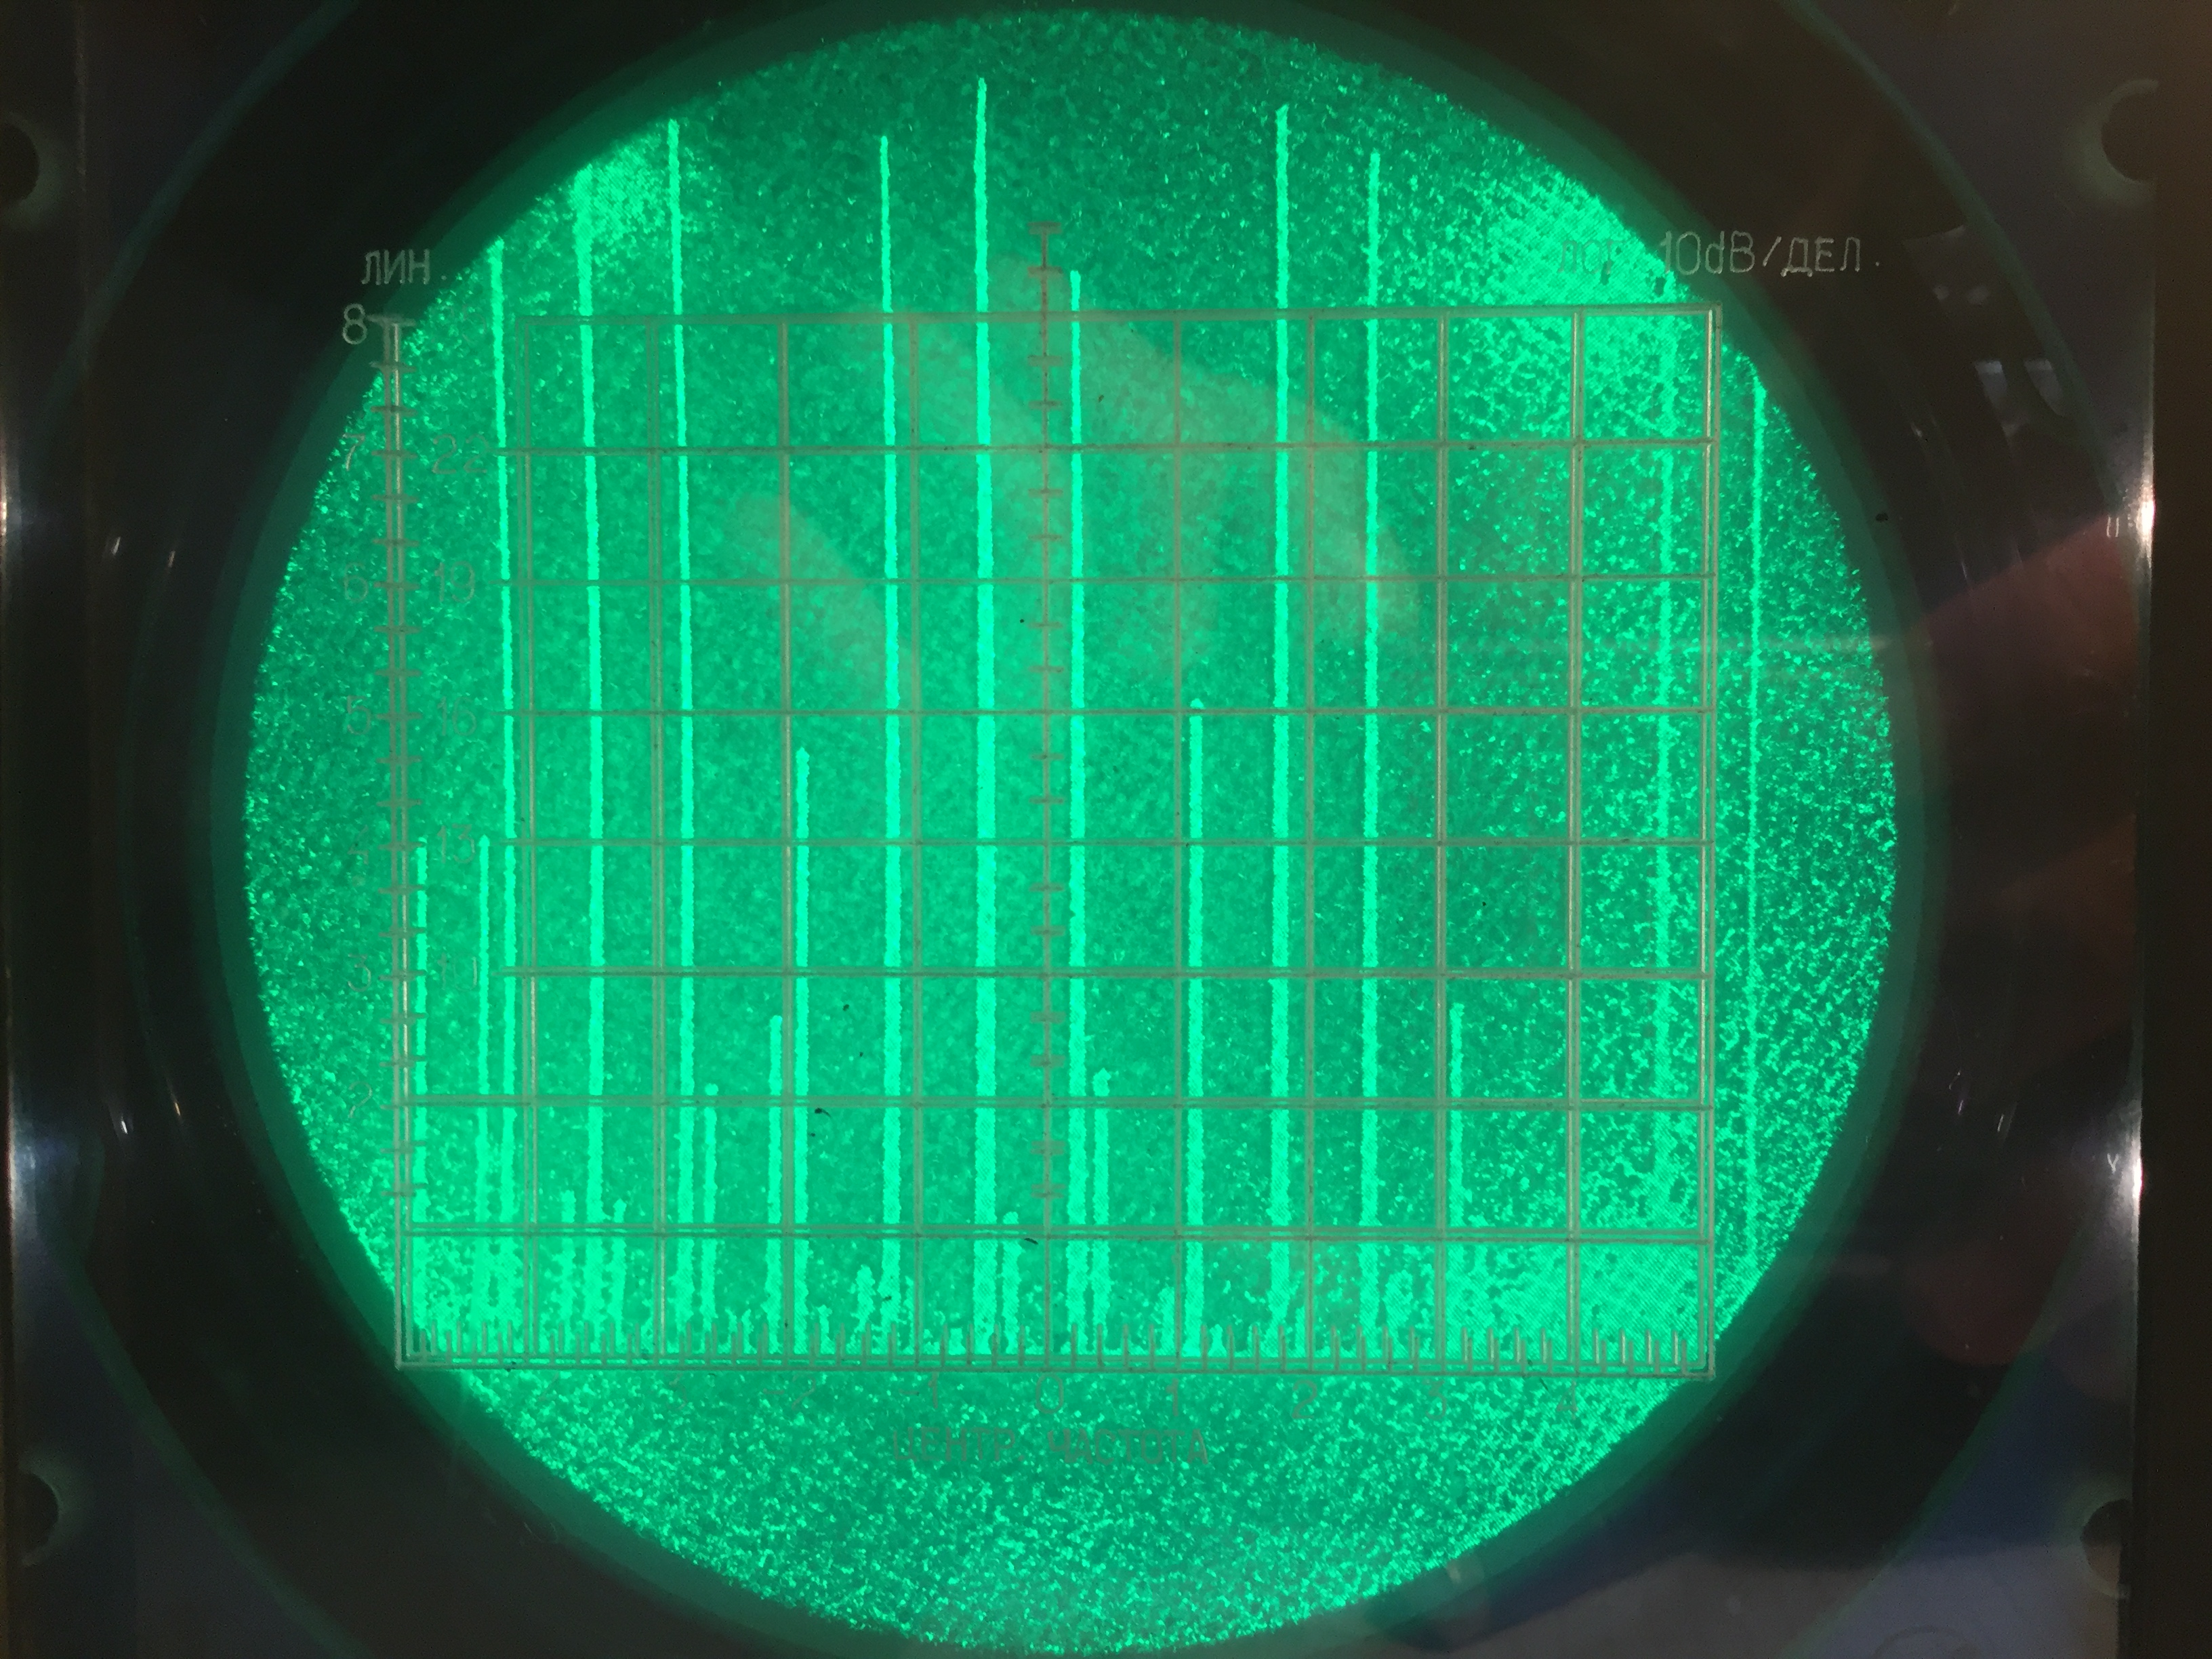
\includegraphics[width=0.9\linewidth]{IMG_0705}} \\ 
	\end{minipage}
	
	\caption{Изменение спектра при увеличении частоты модулирующего сигнала(100$\%$ глубина модуляции).}
	\label{ris:image12}
\end{figure}

\section{Вывод}

Экспериментально было проверено соотношение неопределенности в случае периодической последовательности прямоугольных импульсов и цугов гармонических колебаний. Точность достаточно высокая, полученные значения соответствуют ожиданиям. Основной вклад в погрешность вносит отсутствие мелких делений на анализаторе спектра.

В третьем эксперименте была проверена зависимость отношения амплитуд спектральных линий синусоидального сигнала, модулированного низкочастотными гармоническими колебаниями, от коэффициента модуляции.
\end{document}